%%%% main.tex, 2022/08/10, 2.5
%%%% Copyright (C) 2020 Vinicius Pegorini (vinicius@utfpr.edu.br)
%%
%% This work may be distributed and/or modified under the conditions of the
%% LaTeX Project Public License, either version 1.3 of this license or (at your
%% option) any later version.
%% The latest version of this license is in
%%   http://www.latex-project.org/lppl.txt
%% and version 1.3 or later is part of all distributions of LaTeX version
%% 2005/12/01 or later.
%%
%% This work has the LPPL maintenance status `maintained'.
%%
%% The Current Maintainer of this work is Vinicius Pegorini.
%%
%% This work consists of the files utfprpb.cls, utfprpb.tex, and
%% utfprpb-dados.tex.
%%
%% The Current Maintainer of this work is Vinicius Pegorini.
%% Updated by:
%% - Marco Aurélio Graciotto Silva;
%% - Rogério Aparecido Gonçalves;
%% - Luiz Arthur Feitosa dos Santos.
%%
%% This work consists of the files utfpr.cls, main.tex, and
%% variaveis.tex.
%% A brief description of this work is in readme.md.

%% ####################################################
%%
%% >> Atenção - Leia isso antes de usar esse template<< 
%%
%% Esse template foi desenvolvido por professores,  com a intenção de ajudar os alunos com as entregas na biblioteca. Não há uma equipe especializada e dedicada mantendo tal template, mas sim professores trabalhando além das suas funções básicas, que são: ensino, pesquisa e extensão.
%
%% Também os mantenedores deste template não são especializados em LaTeX, muito menos em normas da ABNT. Todos que contribuíram com o template fizeram isso visando deixá-lo o mais próximo possível das normas da ABNT e das regras, anseios e expectativas da biblioteca da UTFPR. É muito importante entender que os desenvolvedores do template não têm relação direta com a biblioteca ou com a ABNT. Ou seja, não são os desenvolvedores do template que ditam as regras e normas dos textos que devem ser entregues à biblioteca.

%%É válido informar também, que como não há uma equipe dedicada e especializada, o tempo para colaborar com o template é curto. Desta forma, pode ser que não sejam empregadas as melhores técnicas, métodos e ferramentas para o desenvolvimento do template. Também pode acontecer do template não atender completamente todos os anseios e exigências da ABNT e da biblioteca, pois por exemplo, muitas regras de redação possuem questões interpretativas. Assim, o template sempre estará em contínua evolução e seria extremamente interessante que as pessoas (alunos,  professores,  técnicos e entusiastas) colaborarem com a evolução do template. Toda ajuda será bem vinda! Isso pode ser feito enviando e-mail para os desenvolvedores, desta forma, assim que possível esses vão tentar melhorar o template.

%%O template é apenas mais uma ferramenta para o desenvolvimento de trabalhos para a biblioteca. Todavia, podem existir outros templates LaTeX. Assim como há templates em outros formatos, que não o LaTeX. O mais importante é que qualquer pessoa, utilizando a princípio qualquer ferramenta, pode desenvolver textos que atendem os requisitos da biblioteca apenas estudando, interpretando e seguindo as regras da UTFPR e da ABNT, que estão disponíveis na página Web da instituição. O template é só um facilitador.

%%Por fim,  é necessário entender que infelizmente o ambiente LaTeX pode ser complexo e gerar resultados distintos dependendo do: sistema operacional,  pacotes LaTeX utilizados,  configurações alteradas, editor utilizado, a forma que está sendo redigida textos, figuras,  etc. Assim não há como garantir que o resultado final será o esperado.  Dito tudo isso,  >>UTILIZE ESSE TEMPLATE POR SUA CONTA E RISCO<<. Os desenvolvedores e colaboradores deste template não se responsabilizam pelo resultado do uso deste template e se eximem de qualquer responsabilidade.

%###################################################


% Luiz - pdfa: inclusão do pdfa
\PassOptionsToPackage{
	pdfa
}{hyperref}

%% Classe e opções de documento
\documentclass[%% Opções
%% -- Opções da classe memoir --
  12pt,%% Tamanho da fonte: 10pt, 11pt, 12pt, etc.
  a4paper,%% Tamanho do papel: a4paper (A4), letterpaper (carta), etc.
  % fleqn,%% Alinhamento das equações à esquerda (comente para alinhamento centralizado)
  % leqno,%% Numeração das equações no lado esquerdo (comente para lado direito)
  oneside,%% Impressão dos elementos textuais e pós-textuais: oneside (anverso) ou twoside (anverso e verso, se mais de 100 p.)
  openright,%% Impressão da primeira página dos capítulos: openright (anverso), openleft (verso) ou openany (anverso e verso)
%% -- Opções da classe abntex2 --
  sumario = abnt-6027-2012,%% Formatação do sumário: tradicional (estilo tradicional) ou abnt-6027-2012 (norma ABNT 6027-2012)
  chapter = TITLE,%% Títulos de capítulos em maiúsculas (comente para desabilitar)
  % luiz - comentar section para ser minusculo
  %section = TITLE,%% Títulos de seções secundárias em maiúsculas (comente para desabilitar)
  % subsection = TITLE,%% Títulos de seções terciárias em maiúsculas (comente para desabilitar)
  % subsubsection = TITLE,%% Títulos de seções quartenárias em maiúsculas (comente para desabilitar),
%% -- Opções da classe utfprpgtex --
  pretextualoneside,%% Impressão dos elementos pré  -textuais: pretextualoneside (anverso) ou pretextualtwoside (anverso e verso)
  fontetimes,%% Fonte do texto: fontetimes (times), fontearial (arial) ou fontecourier (courier)
  % vinculoscoloridos,%% Cores nos vínculos (citações, arquivos, links, url, etc.) (comente para desabilitar)
  semrecuonosumario,%% Remoção do recuo dos itens no sumário (comente para adição do recuo, se estilo tradicional)
  usemakeindex,%% Compilação de glossários e índices utilizando makeindex (comente para desabilitar)
  % legendascentralizadas,%% Alinhamento das legendas centralizado (comente para alinhamento à esquerda)
  %aprovacaoestiloppg,%% Folha de aprovação do programa de pós-graduação no estilo do PPG (comente para estilo padrão)
  pardeassinaturas,%% Assinaturas na folha de aprovação em até duas colunas (comente para em uma única coluna)
  % linhasdeassinaturas,%% Linhas de assinaturas na folha de aprovação (comente para remover as linhas)
%% -- Opções do pacote babel --
  english,%% Idioma adicional para hifenização
  french,%% Idioma adicional para hifenização
  spanish,%% Idioma adicional para hifenização
  brazil,%% Idioma principal do documento (último da lista)
]{utfpr}%% Classe utfpr

% Luiz: pdfa: necessário para criar pdfa
\usepackage[a-3b,mathxmp]{pdfx}[2018/12/22] % você pode escolher entre a-1b, a-2b, a-3b - o template ainda não suporta o a-Xa de 

%%%% configuracoes.tex, 2022/05/02, 2.4a

%% ####################################################
%%
%% >> Atenção - Leia isso antes de usar esse template<< 
%%
%% Esse template foi desenvolvido por professores,  com a intenção de ajudar os alunos com as entregas na biblioteca. Não há uma equipe especializada e dedicada mantendo tal template, mas sim professores trabalhando além das suas funções básicas, que são: ensino, pesquisa e extensão.
%
%% Também os mantenedores deste template não são especializados em LaTeX, muito menos em normas da ABNT. Todos que contribuíram com o template fizeram isso visando deixá-lo o mais próximo possível das normas da ABNT e das regras, anseios e expectativas da biblioteca da UTFPR. É muito importante entender que os desenvolvedores do template não têm relação direta com a biblioteca ou com a ABNT. Ou seja, não são os desenvolvedores do template que ditam as regras e normas dos textos que devem ser entregues à biblioteca.

%%É válido informar também, que como não há uma equipe dedicada e especializada, o tempo para colaborar com o template é curto. Desta forma, pode ser que não sejam empregadas as melhores técnicas, métodos e ferramentas para o desenvolvimento do template. Também pode acontecer do template não atender completamente todos os anseios e exigências da ABNT e da biblioteca, pois por exemplo, muitas regras de redação possuem questões interpretativas. Assim, o template sempre estará em contínua evolução e seria extremamente interessante que as pessoas (alunos,  professores,  técnicos e entusiastas) colaborarem com a evolução do template. Toda ajuda será bem vinda! Isso pode ser feito enviando e-mail para os desenvolvedores, desta forma, assim que possível esses vão tentar melhorar o template.

%%O template é apenas mais uma ferramenta para o desenvolvimento de trabalhos para a biblioteca. Todavia, podem existir outros templates LaTeX. Assim como há templates em outros formatos, que não o LaTeX. O mais importante é que qualquer pessoa, utilizando a princípio qualquer ferramenta, pode desenvolver textos que atendem os requisitos da biblioteca apenas estudando, interpretando e seguindo as regras da UTFPR e da ABNT, que estão disponíveis na página Web da instituição. O template é só um facilitador.

%%Por fim,  é necessário entender que infelizmente o ambiente LaTeX pode ser complexo e gerar resultados distintos dependendo do: sistema operacional,  pacotes LaTeX utilizados,  configurações alteradas, editor utilizado, a forma que está sendo redigida textos, figuras,  etc. Assim não há como garantir que o resultado final será o esperado.  Dito tudo isso,  >>UTILIZE ESSE TEMPLATE POR SUA CONTA E RISCO<<. Os desenvolvedores e colaboradores deste template não se responsabilizam pelo resultado do uso deste template e se eximem de qualquer responsabilidade.

%###################################################

%% Pacotes carregados nas classes:
%%   memoir: abstract, appendix, array, booktabs, ccaption, chngcntr, chngpage, dcolumn, delarray, enumerate, epigraph, framed,
%%           ifmtarg, ifpdf, index, makeidx, moreverb, needspace, newfile, nextpage, parskip, patchcmd, setspace, shortvrb, showidx,
%%           tabularx, titleref, titling, tocbibind, tocloft, verbatim, verse.
%%   memoir (similares): crop, fancyhdr, geometry, sidecap, subfigure, titlesec.
%%   abntex2: babel, bookmark, calc, enumitem, ifthen, hyperref, textcase.
%%   utfprpgtex: abntex2cite, ae, algorithmic, amsmath, backref, breakurl, caption, cmap, color, eepic, epic, epsfig, etoolbox,
%%               fancyhdr, fix-cm, fontenc, glossaries, graphics, graphicx, helvet, hyphenat, indentfirst, inputenc, lastpage,
%%               morewrites, nomencl, sfmath, sistyle, substr, times, xtab.


%% Pacotes adicionais (\usepackage[options]{package})
\usepackage{bigdelim, booktabs, colortbl, longtable, multirow}%% Ferramentas para tabelas
\usepackage{amssymb, amstext, amsthm, icomma}%% Ferramentas para linguagem matemática
\usepackage{pifont, textcomp, wasysym}%% Símbolos de texto
\usepackage{lipsum}				% para geração de dummy text
\usepackage{subfig}             % para adicionar figuras lado a lado no texto                    
\usepackage{pdfpages}           % para adicionar documentos pdf ao trabalho
\usepackage{xspace}


% luiz: primeira letra maiúscula
% solução 1
%\usepackage{stringstrings}
%\newcommand{\firstcap}[1]{\caselower[e]{#1}\capitalize{\thestring}}

% solução 2 - não usei essa
% \usepackage[utf8]{inputenc}
% \usepackage{datatool-base}
% \usepackage{mfirstuc}

% Formatação do título da seção - primeira letra caixa alta e o resto em caixa baixa.
% \usepackage[explicit]{titlesec}
% \usepackage{lipsum}
% \titleformat{\section}{\normalfont}{\thesection}{1em}{\textbf{\firstcap{#1}}} % funciona mas apenas para o título da seção e não para o sumário (a configuração do sumário está mais para baixo

% luiz: define o underline colorido.
% https://github.com/abntex/abntex2-contrib/blob/master/customizacoes/pucminas/abntex2-pucminas.sty
% acabei não usando o black e o coloruline da solução do link

\usepackage[normalem]{ulem} % para o underline colorido na seção quaternária
\renewcommand*{\cftsubsubsectionfont}{\normalfont\uline} % underline no sumário
\setsubsubsecheadstyle{\ABNTEXsubsubsectionfont\ABNTEXsubsubsectionfontsize\ABNTEXsubsubsectionupperifneeded\uline} %underline no título da subsubsection

% luiz: bibliografia - opções

%% Comandos personalizados (\newcommand{name}[num]{definition})
\newcommand{\cpp}{\texttt{C$++$}}%% C++
\newcommand{\latex}{\LaTeX\xspace}%% LaTeX
\newcommand{\ds}{\displaystyle}%% Tamanho normal das equações
\newcommand{\bsym}[1]{\boldsymbol{#1}}%% Texto no modo matemático em negrito
\newcommand{\mr}[1]{\mathrm{#1}}%% Texto no modo matemático normal (não itálico)
\newcommand{\der}{\mr{d}}%% Operador diferencial
\newcommand{\deri}[2]{\frac{\der #1}{\der #2}}%% Derivada ordinária
\newcommand{\derip}[2]{\frac{\partial #1}{\partial #2}}%% Derivada parcial
\newcommand{\pare}[1]{\left( #1 \right)}%% Parênteses
\newcommand{\colc}[1]{\left[ #1 \right]}%% Colchetes
\newcommand{\chav}[1]{\left\lbrace #1 \right\rbrace}%% Chaves
\newcommand{\sen}{\operatorname{sen}}%% Operador seno
\newcommand{\senh}{\operatorname{senh}}%% Operador seno hiperbólico
\newcommand{\tg}{\operatorname{tg}}%% Operador tangente
\newcommand{\tgh}{\operatorname{tgh}}%% Operador tangente hiperbólico
\newcommand{\seqref}[1]{Equação~\eqref{#1}}%% Referência de uma única equação
\newcommand{\meqref}[1]{Equações~\eqref{#1}}%% Referência de múltiplas equações
\newcommand{\citep}[1]{\cite{#1}}%% Atalho para citação implícita
\newcommand{\citet}[1]{\citeonline{#1}}%% Atalho para citação explícita
\newcommand{\citepa}[1]{(\citeauthor{#1})}%% Atalho para citação implícita (somente autor)
\newcommand{\citeta}[1]{\citeauthoronline{#1}}%% Atalho para citação explícita (somente autor)
\newcommand{\citepy}[1]{(\citeyear{#1})}%% Atalho para citação implícita (somente ano)
\newcommand{\citety}[1]{\citeyear{#1}}%% Atalho para citação explícita (somente ano)

\newcommand{\fonteTexto}[1]{\renewcommand{\familydefault}{#1}}

% Define o caminho das figuras
\graphicspath{{figuras/}}

% Define a fonte ara helvet que é uma fonte similar à Arial, se for usar a Arial tem que mudar o compilador para XeLaTex, mas ai tem que arrumar os erros: https://latex.org/forum/viewtopic.php?t=25998
%\usepackage{helvet}
%\renewcommand{\familydefault}{\sfdefault}
%\usepackage{times} % para fonte time new roman
%\usepackage{pslatex} % ou essa aqui...

%\usepackage{titlesec}

%% Configuração de glossário
% \usepackage[portuguese]{nomencl}
% \usepackage[nogroupskip,nonumberlist,nopostdot,nohypertypes={acronym}]{glossaries}
% \makenoidxglossaries
\usepackage{glossaries}
\makeglossaries

% para siglas em português
\newcommand{\siglaPt}[2]
{
 \newglossaryentry{#1}{
  name=#1,
  description={#2},
  first={#2 (#1)},
  long={#2}
 }  
}

% para siglas de língua estrangeira, nessas a descrição longa fica em itálico.
\newcommand{\siglaIt}[2]
{
 \newglossaryentry{#1}{
  name=#1,
  description={\textit{#2}},
  first={\textit{#2} ({#1})},
  long={\textit{#2}}
 }  
}

%% luiz - para fazer os avisos
\usepackage{tcolorbox}

% use para criar caixas de avisos, pode ser utilizado para fazer anotações de tarefas indicadas pelo orientador/banca.
% \caixa{Atenção}{texto...}
\newcommand{\caixa}[2]{
\begin{tcolorbox}[colback=red!5!white,colframe=red!45!white, title = #1, fonttitle=\bfseries]
#2
\end{tcolorbox}
}

% Luiz - Linhas órfãs e viúvas
\widowpenalty=10000
\clubpenalty=10000

% Luiz - Caption do tamanho da Tabela
%\usepackage[width=1\textwidth]{caption}

% Luiz - configurar a margem dos itens
\setlength{\leftmargini}{1.5cm}
\setlength{\leftmarginii}{1.5cm}


%% Arquivo de dados do modelo de documento LaTeX para produção de trabalhos acadêmicos da UTFPR
%%%% variaveis.tex, 2022/05/02, 2.4a
%%%% Copyright (C) 2020 Vinicius Pegorini (vinicius@utfpr.edu.br)
%%
%% This work may be distributed and/or modified under the conditions of the
%% LaTeX Project Public License, either version 1.3 of this license or (at your
%% option) any later version.
%% The latest version of this license is in
%%   http://www.latex-project.org/lppl.txt
%% and version 1.3 or later is part of all distributions of LaTeX version
%% 2005/12/01 or later.
%%
%% This work has the LPPL maintenance status `maintained'.
%%
%% The Current Maintainer of this work is Vinicius Pegorini.
%% Updated by:
%% - Marco Aurélio Graciotto Silva;
%% - Rogério Aparecido Gonçalves;
%% - Luiz Arthur Feitosa dos Santos.
%%
%% This work consists of the files utfpr.cls, main.tex, and
%% variaveis.tex.
%%
%% A brief description of this work is in readme.txt.

%% ####################################################
%%
%% >> Atenção - Leia isso antes de usar esse template<< 
%%
%% Esse template foi desenvolvido por professores,  com a intenção de ajudar os alunos com as entregas na biblioteca. Não há uma equipe especializada e dedicada mantendo tal template, mas sim professores trabalhando além das suas funções básicas, que são: ensino, pesquisa e extensão.
%
%% Também os mantenedores deste template não são especializados em LaTeX, muito menos em normas da ABNT. Todos que contribuíram com o template fizeram isso visando deixá-lo o mais próximo possível das normas da ABNT e das regras, anseios e expectativas da biblioteca da UTFPR. É muito importante entender que os desenvolvedores do template não têm relação direta com a biblioteca ou com a ABNT. Ou seja, não são os desenvolvedores do template que ditam as regras e normas dos textos que devem ser entregues à biblioteca.

%%É válido informar também, que como não há uma equipe dedicada e especializada, o tempo para colaborar com o template é curto. Desta forma, pode ser que não sejam empregadas as melhores técnicas, métodos e ferramentas para o desenvolvimento do template. Também pode acontecer do template não atender completamente todos os anseios e exigências da ABNT e da biblioteca, pois por exemplo, muitas regras de redação possuem questões interpretativas. Assim, o template sempre estará em contínua evolução e seria extremamente interessante que as pessoas (alunos,  professores,  técnicos e entusiastas) colaborarem com a evolução do template. Toda ajuda será bem vinda! Isso pode ser feito enviando e-mail para os desenvolvedores, desta forma, assim que possível esses vão tentar melhorar o template.

%%O template é apenas mais uma ferramenta para o desenvolvimento de trabalhos para a biblioteca. Todavia, podem existir outros templates LaTeX. Assim como há templates em outros formatos, que não o LaTeX. O mais importante é que qualquer pessoa, utilizando a princípio qualquer ferramenta, pode desenvolver textos que atendem os requisitos da biblioteca apenas estudando, interpretando e seguindo as regras da UTFPR e da ABNT, que estão disponíveis na página Web da instituição. O template é só um facilitador.

%%Por fim,  é necessário entender que infelizmente o ambiente LaTeX pode ser complexo e gerar resultados distintos dependendo do: sistema operacional,  pacotes LaTeX utilizados,  configurações alteradas, editor utilizado, a forma que está sendo redigida textos, figuras,  etc. Assim não há como garantir que o resultado final será o esperado.  Dito tudo isso,  >>UTILIZE ESSE TEMPLATE POR SUA CONTA E RISCO<<. Os desenvolvedores e colaboradores deste template não se responsabilizam pelo resultado do uso deste template e se eximem de qualquer responsabilidade.

%###################################################

%% Documento
%% Luiz: Define a fonte do texto da monografia
\fonteTexto{\sfdefault} % utilize \rmdefault para Times New Roman ou \sfdefault para Arial
\TipoDeDocumento{Trabalho de Conclusão de Curso de Graduação}%% Tipo de documento: "Tese", "Dissertação" ou "Trabalho de Conclusão de Curso de Graduação", "Estágio Supervisionado"
\NivelDeFormacao{Tecnólogo}%% Nível de formação: "Doutorado", "Mestrado", "Bacharelado" ou "Tecnólogo" - ATENÇÃO, isso será utilizado para alterar a formatação do trabalho, pois pode haver formatações distintas dependendo o nível/tipo de trabalho.


%% luiz
% Template LaTex criado pelo Departamento Acadêmico de Computação (DACOM)
% da Universidade Tecnológica Federal do Paraná - Campus Campo Mourão (UTFPR-CM)
% Criado e alterado pelos professores:
% - Marco Aurélio Graciotto Silva
% - Rogério Aparecido Gonçalvez
% - Luiz Arthur Feitosa dos Santos
% Esse template utiliza a licença CC BY:
% Esta licença permite que outros distribuam, remixem, adaptem e criem a partir deste trabalho, mesmo para fins comerciais, desde que atribuam o devido crédito pela criação original.
% https://creativecommons.org/licenses/by/4.0/deed.pt_BR

% Dados do curso. Caso seja BCC:
% \program{Curso de Bacharelado em Ciência da Computação}
% \programen{Undergradute Program in Computer Science}
% \degree{Bacharel}
% \degreearea{Ciência da Computação}
% Caso seja TSI:
\program{Curso Superior de Tecnologia em Sistemas para Internet}
\programen{Undergradute Program in Tecnology for Internet Systems}
\degree{Tecnólogo}
\degreearea{Tecnologia em Sistemas para Internet}


% Dados da disciplina. Escolha uma das opções e a descomente:
% TCC1:
\goal{Proposta de Trabalho de Conclusão de Curso de Graduação}
\course{Trabalho de Conclusão de Curso 1}
% TCC2:
%  \goal{Trabalho de Conclusão de Curso de Graduação}
%  \course{Trabalho de Conclusão de Curso 2}


% Dados do TCC (precisa alterar)
\author{Guilherme Minozzi}  % Seu nome
\authorbib{Minozzi, Guilherme} % Seu nome para referência bibliográfica (Sobrenome, Nome)
% ToDo: Alterar o título, após sanar dúvidas com o orientador
\title{CLIENTE WEB PARA BALANCEAMENTO NUTRICIONAL E GERENCIAMENTO DO GADO LEITEIRO} % Título do trabalho
\titleen{Put your english title here} % Título traduzido para inglês
\advisor{Prof. Me. Vinicius Pegorini} % Nome do orientador. Lembre-se de prefixar com "Prof. Dr.", "Profª. Drª.", "Prof. Me." ou "Profª. Me."}
% Se não houver corientador, comente a linha a baixo
% \coadvisor{Nome Orientador completo e título} % Nome do coorientador, caso exista. Caso não exista, comente a linha.
\depositshortdate{2023} % Ano em que depositou este documento
% ToDo: Alterar a data de aprovação
\approvaldate{01/janeiro/2021}

% Dados do curso que não precisam de alteração
\university{Universidade Tecnológica Federal do Paraná}
\universityen{Federal University of Technology -- Paraná}
\universitycampus{Campus Campo Mourão}
\universityunit{Departamento Acadêmico de Computação}
\address{Pato Branco}
\addressen{Campo Mourão, PR, Brazil}
\documenttype{Monografia}
\documenttypeen{Monograph}
\degreetype{Graduação}

% ToDo: Quem seriam os membros?
\evalboardmember{Nome completo e por extenso do Membro 1}{Título (especialização, mestrado, doutorado}{Nome completo e por extenso da instituição a qual possui vínculo}
\evalboardmember{Nome completo e por extenso do Membro 2}{Título (especialização, mestrado, doutorado}{Nome completo e por extenso da instituição a qual possui vínculo}
\evalboardmember{Nome completo e por extenso do Membro 3}{Título (especialização, mestrado, doutorado}{Nome completo e por extenso da instituição a qual possui vínculo}
\evalboardmember{Nome completo e por extenso do Membro 4}{Título (especialização, mestrado, doutorado}{Nome completo e por extenso da instituição a qual possui vínculo}

%% Palavras-chave e keywords
%% ATENÇÃO - você deve indicar a quantidade de palavras chaves para o template LaTeX utilizar o pontuação correta!
\NumeroDePalavrasChave{5}%% Número de palavras-chave (máximo 5)
%% Atenção - por enquanto o template não está suportando acentos normais na palavra chave, por isso caso a palavra tenha acento, você deve utilizar o estilo antigo do LaTeX, sendo os acentos: á - \'a  é - \'e   â - \^a  ê - \^e  à - \`a  ä - \"a  ç - \c{c}
% ToDo: Alterar as palavras chaves
\PalavraChaveA{Palavra-chave 1}%% Palavra-chave A
\PalavraChaveB{Palavra-chave 2}%% Palavra-chave B
\PalavraChaveC{Palavra-chave 3}%% Palavra-chave C
\PalavraChaveD{Palavra-chave 4}%% Palavra-chave D
\PalavraChaveE{Palavra-chave 5}%% Palavra-chave E
%% Exemplo de como utilizar acentos na Palavra-chave:
% \PalavraChaveA{ol\'a}%% Olá
%\PalavraChaveB{voc\^e}%% você
%\PalavraChaveC{\`a}%% à
%\PalavraChaveD{a\c{c}\~ao}%% ação
%\PalavraChaveE{arg\"uir}%% argüir


%% ATENÇÃO - você deve indicar a quantidade de keywords para o template LaTeX utilizar o pontuação correta!
\NumeroDeKeywords{5}%% Número de keywords (máximo 5)
\KeywordA{Keyword 1}%% Keyword A
\KeywordB{Keyword 2}%% Keyword B
\KeywordC{Keyword 3}%% Keyword C
\KeywordD{Keyword 4}%% Keyword D
\KeywordE{Keyword 5}%% Keyword E


% É obrigatório o uso de uma licença Creative Commons (CC) nos trabalhos de TCC pelos cursos ligados a DACOM da UTFPR-CM.
% Veja: http://portal.utfpr.edu.br/biblioteca/trabalhos-academicos/docentes/procedimento-de-entrega-graduacao

% Sendo assim, escolha com o seu orientador uma das licenças CC a seguir: 

% CC BY: Esta licença permite que outros distribuam, remixem, adaptem e criem a partir deste trabalho, mesmo para fins comerciais, desde que atribuam o devido crédito pela criação original. Essa é a menos restritiva.
\licenca{ccby}

% CC BY CA: Esta licença permite que outros remixem, adaptem e criem a partir deste trabalho, mesmo para fins comerciais, desde que atribuam o devido crédito e que licenciem as novas criações sob termos idênticos.
%\licenca{ccbysa}

% CC BY ND: Esta licença permite a redistribuição, comercial e não comercial, desde que o trabalho seja distribuído inalterado e no seu todo, com crédito ao autor.
%\licenca{ccbynd}

% CC BY NC: Esta licença permite que outros remixem, adaptem e criem a partir deste trabalho para fins não comerciais, e embora os novos trabalhos tenham de atribuir o devido crédito e não possam ser usados para fins comerciais, os trabalhos derivados não têm que serem licenciados sob os mesmos termos.
%\licenca{ccbync}

% CC BY NC SA: Esta licença permite que outros remixem, adaptem e criem a partir deste trabalho para fins não comerciais, desde que atribuam ao autor o devido crédito e que licenciem as novas criações sob termos idênticos.
%\licenca{ccbyncsa}

% CC BY NC ND: Esta licença só permite que outros façam download do trabalho e o compartilhe desde que atribuam crédito ao autor, mas sem que possam alterá-los de nenhuma forma ou utilizá-los para fins comerciais. Essa é a mais restritiva.
%\licenca{ccbyncnd}

% Deixar sem licença - isso é aplicado apenas aos trabalhos que não são obrigados a ter licença. Na duvida verifique isso com o seu orientador e professor responsável pelo TCC. Para deixar o texto sem licença deixe o comando licença em brando ou deixe comentado.
%\licenca{}
% by DACOM/UTFPR-CM%% Realize as modificações pertinentes no arquivo "utfprpb-dados.tex"

%% Ferramenta para criação de índices
\makeindex%% Não comente esta linha

%% Ferramenta para criação de glossários
\makeglossaries%% Não comente esta linha
%%%% LISTA DE ABREVIATURAS E SIGLAS 
%%
%% Relação, em ordem alfabética, das abreviaturas (representação de uma palavra por meio de alguma(s) de sua(s) sílaba(s) ou
%% letra(s)), siglas (conjunto de letras iniciais dos vocábulos e/ou números que representa um determinado nome) e acrônimos
%% (conjunto de letras iniciais dos vocábulos e/ou números que representa um determinado nome, formando uma palavra pronunciável).
%%
%% Este arquivo para definição de abreviaturas, siglas e acrônimos é utilizado com a opção "glossaries" (pacote)

%% Abreviaturas: \abreviatura{rótulo}{representação}{definição}

\abreviatura{art.}{art.}{Artigo}
\abreviatura{cap.}{cap.}{Capítulo}
\abreviatura{sec.}{sec.}{Seção}

%% Siglas: \sigla{rótulo}{representação}{definição}

\sigla{abnt}{ABNT}{Associação Brasileira de Normas Técnicas}
\sigla{cnpq}{CNPq}{Conselho Nacional de Desenvolvimento Científico e Tecnológico}
\sigla{eps}{EPS}{\textit{Encapsulated PostScript}}
\sigla{pdf}{PDF}{Formato de Documento Portátil, do inglês \textit{Portable Document Format}}
\sigla{ps}{PS}{\textit{PostScript}}
\sigla{utfpr}{UTFPR}{Universidade Tecnológica Federal do Paraná}

% ==================== MINHAS SIGLAS ==========================
\sigla{CNA}{CNA}{Confederação da Agricultura e Pecuária do Brasil}

\sigla{PIB}{PIB}{Produto Interno Bruto}

\sigla{IBGE}{IBGE}{Instituto Brasilerio de Geografia e Estatística}

\sigla{CEPEA}{CEPEA}{Centro de Estudos Avançados em Economia Aplicada}

\sigla{IDR-PR}{IDR-PR}{Instituto de Desenvolvimento Rural do Paraná}

\sigla{API}{API}{Interface de Programação de Aplicativos, do inglês \textit{Application Programming Interface}}

\sigla{REST}{REST}{Transferência de Estado Representacional, do inglês \textit{Representational State Transfer}}
\sigla{CMS}{CMS}{Consumo de Matéria Seca}
\sigla{CNCPS}{CNCPS}{\textit{Cornell Net Carbohydrate and Protein System}}
\sigla{NRC}{NRC}{\textit{National Research Council}}

\sigla{UI}{UI}{Interface do Usuário, do inglês \textit{User Interface}}

\sigla{VSCode}{VS Code}{Visual Studio Code}

\sigla{IDE}{IDE}{Ambiente de Desenvolvimento Integrado, do inglês \textit{Integrated Development Environment}}

\sigla{MVC}{MVC}{\textit{Model-View-Controller}}

\sigla{DOM}{DOM}{\textit{Document Object Model}}

\sigla{BRL}{BRL}{Real Brasileiro}

\sigla{ECC}{ECC}{Escore de Condição Corporal}

\sigla{PB}{PB}{Proteína Bruta}

\sigla{NDT}{NDT}{Nutrientes Digestíveis Totais}

%% LEIA:

%% Para usar o \gls, você deve colocar a sigla aqui em \sigla

%% ADICIONAR SIGLAS: Quando você inclui alguma sigla, pode ser necessário compilar umas duas vezes para essa aparecer na lista de siglas.

%% ATENÇÃO REMOVER SIGLAS: se você remover a sigla do seu texto (não for usar mais), você deve comentar essa aqui e remover os \gls{} dessa sigla (se não vai ficar aparecendo a sigla na lista). Em caso de ERRO, quando o LaTeX informa que você ainda tem a sigla no texto, mesmo que não tenha. Você deve limpar o cache - no OverLeaf, clique no erro, vá:
%  ->view error
%%   ->(role para baixo, até o final)
%%     ->e clique em Clear cached files


%% Acrônimos: \acronimo{rótulo}{representação}{definição}
%\acronimo{gimp}{Gimp}{Programa de Manipulação de Imagem GNU, do inglês \textit{GNU Image Manipulation Program}}
%% Entradas da lista de abreviaturas e siglas - Comente para remover este item
%%%% GLOSSÁRIO
%%
%% Relação de palavras ou expressões técnicas de uso restrito ou de sentido obscuro, utilizadas no texto, acompanhadas das
%% respectivas definições.

%% Entradas do glossário: \newglossaryentry{rótulo}{informações da entrada}

\newglossaryentry{pai}{%% Informações da entrada
  name        = {pai},
  plural      = {pais},
  description = {um exemplo de entrada pai que possui subentradas (entradas filhas)}
}

\newglossaryentry{componente}{%% Informações da entrada
  name        = {componente},
  plural      = {componentes},
  parent      = {pai},
  description = {um exemplo de uma entrada componente, subentrada da entrada chamada \gls{pai}}
}

\newglossaryentry{filho}{%% Informações da entrada
  name        = {filho},
  plural      = {filhos},
  parent      = {pai},
  description = {um exemplo de uma entrada filha (subentrada) da entrada chamada \gls{pai}. Trata-se de uma entrada irmã da entrada chamada \gls{componente}}
}

\newglossaryentry{equilibrio}{%% Informações da entrada
  name        = {equilíbrio da configuração},
  see         = [veja também]{componente},
  description = {uma consistência entre os \glspl{componente}}
}

\newglossaryentry{tex}{%% Informações da entrada
  name        = {\TeX},
  sort        = {TeX},
  description = {é um sistema de tipografia criado por Donald E. Knuth}
}

\newglossaryentry{latex}{%% Informações da entrada
  name        = {\latex},
  sort        = {LaTeX},
  description = {um conjunto de macros para o processador de textos \gls{tex}, utilizado amplamente para a produção de textos matemáticos e científicos devido à sua alta qualidade tipográfica}
}

\newglossaryentry{bibtex}{%% Informações da entrada
  name        = {Bib\TeX},
  sort        = {BibTeX},
  parent      = {latex},
  description = {um software de gerenciamento de referências para a formatação de listas de referências. A ferramenta Bib\TeX\ é normalmente usada em conjunto com o sistema de preparação de documentos do \gls{latex}}
}

\newglossaryentry{abntex2}{%% Informações da entrada
  name        = {\abnTeX},
  sort        = {abnTeX2},
  see         = {latex},
  description = {uma suíte para \gls{latex} que atende os requisitos das normas da Associação Brasileira de Normas Técnicas (ABNT) para elaboração de documentos técnicos e científicos brasileiros, como artigos científicos, relatórios técnicos, trabalhos acadêmicos como teses, dissertações, projetos de pesquisa e outros documentos do gênero}
}

\newglossaryentry{utfprpbtex}{%% Informações da entrada
  name        = {\utfprpbtex},
  sort        = {UTFPRPBTeX},
  see         = {latex},
  parent      = {abntex2},
  description = {uma suíte para \gls{latex}, baseada na suíte \gls{abntex2}, que atende os requisitos das normas definidas pela Universidade Tecnológica Federal do Paraná (UTFPR), Câmpus Pato Branco, para elaboração de trabalhos acadêmicos}
}
%% Entradas do glossário - Comente para remover este item

%% Ferramenta para criação de nomenclaturas
\makenomenclature%% Não comente esta linha

%% Início do documento
\begin{document}%% Não comente esta linha

%% Formatação de páginas de elementos pré-textuais
\pretextual%% Não comente esta linha

%% Capa
%\incluircapa%% Comente para remover este item
\coverpageone

%% Folha de rosto (* coloca a ficha bibliográfica no verso)
%\incluirfolhaderosto*%% Comente para remover este item
\coverpagetwo

% luiz - iniciar contagem depois da folha de rosto
\clearpage
\setcounter{page}{1}

%% Ficha catalográfica (teses e dissertações)
%\incluirfichacatalografica%% Comente para remover este item

%% Errata
%%%%% ERRATA
%%
%% Lista dos erros ocorridos no texto, seguidos das devidas correções.

\begin{errata}%% Ambiente errata
\begin{table*}[htb]%% Ambiente table
\begin{tabularx}{\textwidth}{|l|l|X|X|}%% Ambiente tabularx
\hline
\textbf{Página(s)}         & \textbf{Linha(s)} & \textbf{Onde se lê} & \textbf{Leia-se}         \\ \hline
\pageref*{errata:capitulo} & 4, 9-11, 14-16    & capítulo(s)         & seção(ões) primária(s)   \\ \hline
\pageref*{errata:secao}    & 12-16             & seção(ões)          & seção(ões) secundária(s) \\ \hline
\pageref*{errata:subsecao} & 16                & subseção(ões)       & seção(ões) terciária(s)  \\ \hline
\end{tabularx}
\end{table*}
\end{errata}
%% Comente para remover este item

%% Folha de aprovação
%\incluirfolhaaprovacao
\approvalpage
%\incluirfolhadeaprovacao%% Para adicionar no formato de texto
%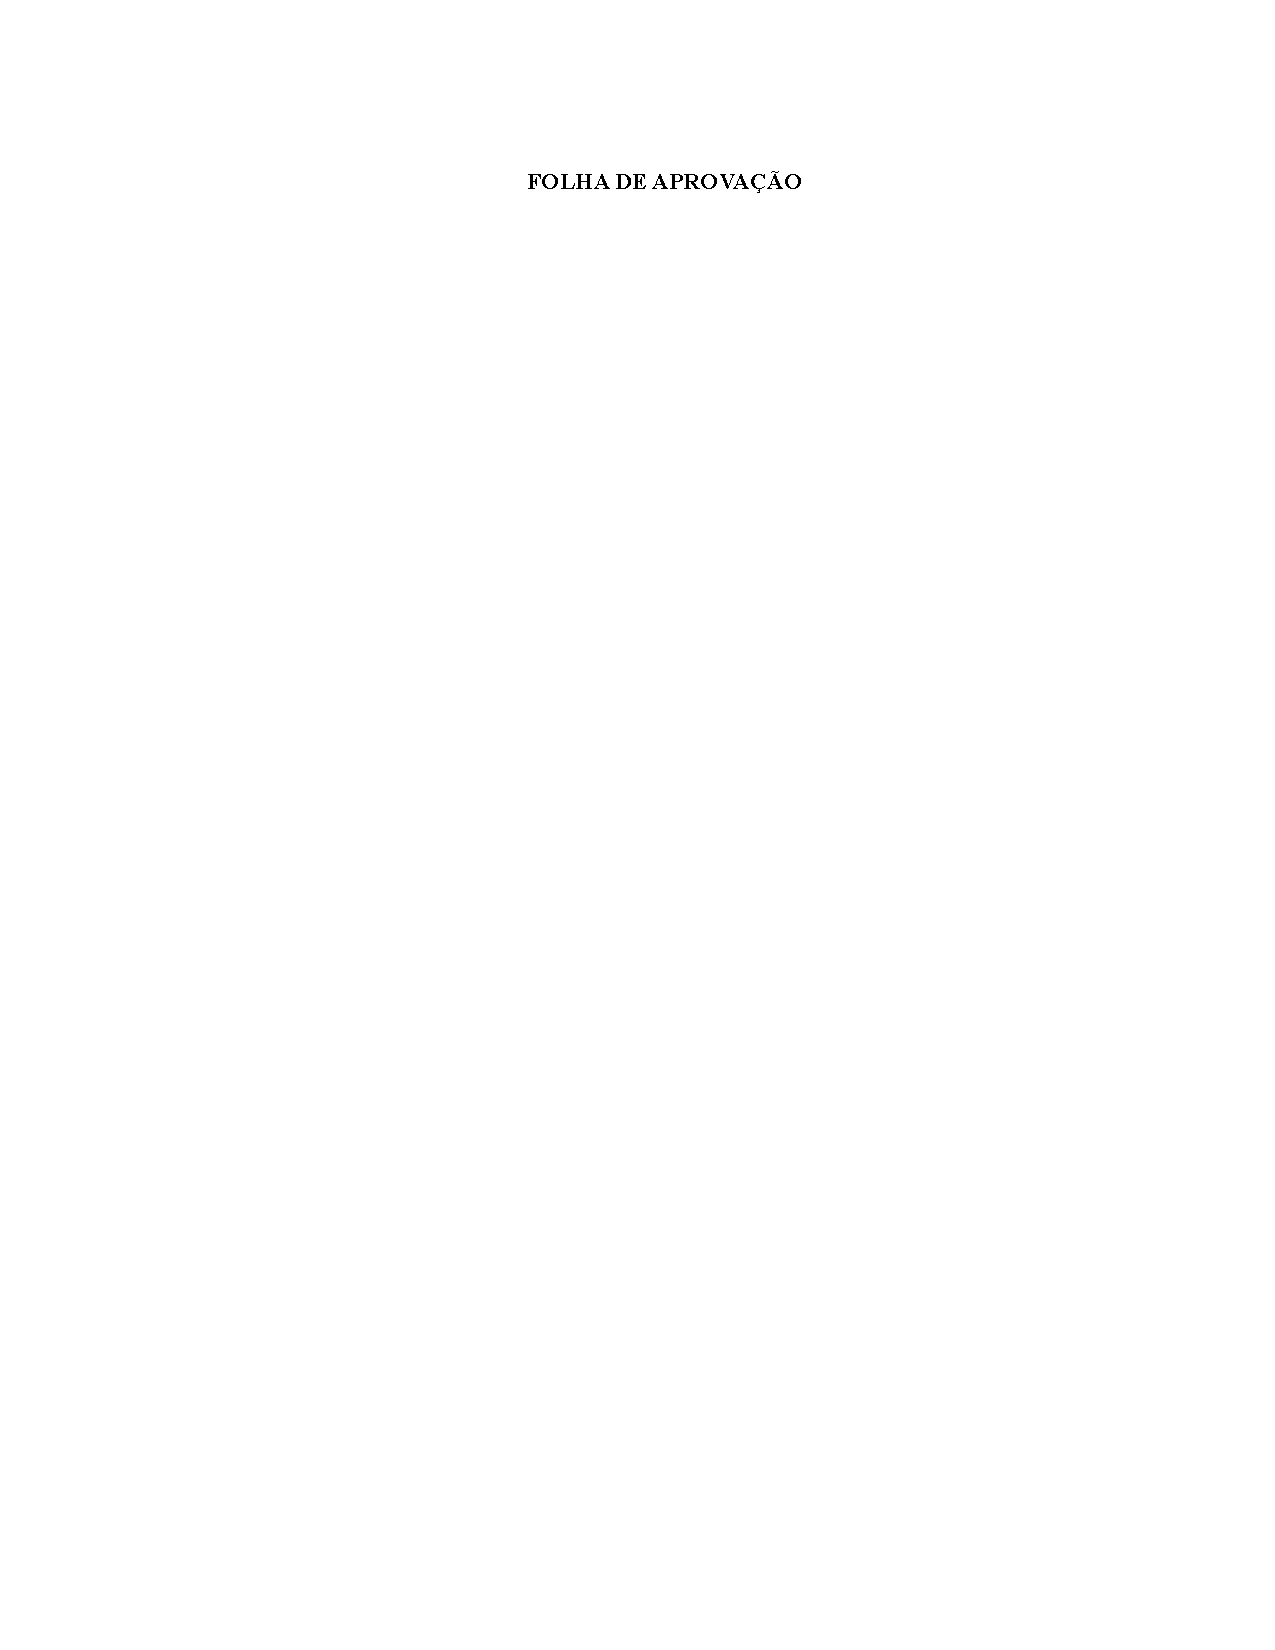
\includepdf[scale=1.0,pages=1]{./PreTexto/folha-aprovacao.pdf} % para adicionar o pdf enviado pelo professor apenas substitua o documento folha-aprovacao.pdf dentro da pasta PreTexto

%% Dedicatória
% %%%% DEDICATÓRIA
%%
%% Texto em que o autor presta homenagem ou dedica seu trabalho.

\begin{dedicatoria}%% Ambiente dedicatoria

Espaço destinado à dedicatória (elemento opcional).
Folha que contém o oferecimento do trabalho à determinada pessoa ou pessoas. Exemplo:

Dedico este trabalho à minha família, pelos momentos de ausência.

\end{dedicatoria}
%% Comente para remover este item

%% Agradecimentos
% %%%% AGRADECIMENTOS
%%
%% Texto em que o autor faz agradecimentos dirigidos àqueles que contribuíram de maneira relevante à elaboração do trabalho.

\begin{agradecimentos}%% Ambiente agradecimentos

Certamente estes parágrafos não irão atender a todas as pessoas que fizeram parte dessa importante fase de minha vida. Portanto, desde já peço desculpas àquelas que não estão presentes entre essas palavras, mas elas podem estar certas que fazem parte do meu pensamento e de minha gratidão. 

Agradeço ao(a) meu(minha) orientador(a) Prof.(a) Dr.(a) Nome Completo, pela sabedoria com que me guiou nesta trajetória.

Aos meus colegas de sala.

A Secretaria do Curso, pela cooperação.

Gostaria de deixar registrado também, o meu reconhecimento à minha família, pois acredito que sem o apoio deles seria muito difícil vencer esse desafio. 

Enfim, a todos os que por algum motivo contribuíram para a realização desta pesquisa.


Espaço destinado aos agradecimentos (elemento opcional). Folha que contém manifestação de reconhecimento a pessoas e/ou instituições que realmente contribuíram com o(a) autor(a), devendo ser expressos de maneira simples.

Não devem ser incluídas informações que nominem empresas ou instituições não nominadas no trabalho.

Se o aluno recebeu bolsa de fomento à pesquisa, informar o nome completo da agência de fomento. Ex: Capes, CNPq, Fundação Araucária, UTFPR, etc. Incluir o número do projeto após a agência de fomento. Este item deve ser o último.

Atenção: não utilizar este exemplo na versão final. Use a sua criatividade!

\end{agradecimentos}
%% Comente para remover este item

%% Epígrafe
% %%%% EPÍGRAFE
%%
%% Texto em que o autor apresenta uma citação, seguida de indicação de autoria, relacionada com a matéria tratada no corpo do
%% trabalho.

\begin{epigrafe}%% Ambiente epigrafe
Primeira Lei: Um robô não pode ferir um ser humano ou, por omissão, permitir que um ser humano sofra algum mal. Segunda Lei: Um robô deve obedecer as ordens que lhe sejam dadas por seres humanos, exceto nos casos em que tais ordens contrariem a Primeira Lei. Terceira Lei: Um robô deve proteger sua própria existência desde que tal proteção não entre em conflito com a Primeira e Segunda Leis (ASIMOV, Isaac, 1950) - observação: A referência deve ser incluída na lista de referências no final do trabalho.

(elemento opcional)
\end{epigrafe}
%% Comente para remover este item

%% Resumo
%%%% RESUMO
%%
%% Apresentação concisa dos pontos relevantes de um texto, fornecendo uma visão rápida e clara do conteúdo e das conclusões do
%% trabalho.

\begin{resumoutfpr}%% Ambiente resumoutfpr
  O estado do Paraná, como um dos principais contribuintes para a produção nacional de leite, enfrenta desafios na gestão eficaz do rebanho, especialmente no manejo alimentar. Apesar da qualidade garantida da alimentação, muitas vezes, ela não atende às necessidades nutricionais do gado leiteiro. Nesse contexto, propõe-se um sistema web para otimizar o tratamento e armazenamento de dados relacionados ao rebanho e alimentação. O objetivo central do sistema é aprimorar a eficiência na gestão do rebanho, proporcionando uma abordagem mais eficaz para a alimentação e nutrição do gado, visando melhoras significativas na produção leiteira. Destinado a auxiliar técnicos do \gls{IDR-PR} e produtores, o sistema abrange a gestão dos animais, nutrição, acompanhamento nas propriedades rurais e informações das propriedades. A falta de manejo adequado do rebanho, apesar dos avanços tecnológicos, é evidente, e um sistema robusto pode oferecer uma solução integrada. A metodologia ágil adotada no desenvolvimento do projeto permitirá a adaptação contínua às mudanças de requisitos, proporcionando melhorias com base em \textit{feedbacks} contínuos ao longo dos marcos do projeto. Ao abordar especificamente as necessidades nutricionais dos animais, o sistema busca não apenas armazenar dados, mas também proporcionar uma compreensão aprofundada das práticas atuais dos técnicos do \gls{IDR-PR}, facilitando a tomada de decisões informadas. A sincronização eficiente dos dados entre o cliente web e a API é crucial, considerando os desafios potenciais de conectividade em ambientes rurais.
\end{resumoutfpr}
%% Comente para remover este item

%% Abstract
%%%% ABSTRACT
%%
%% Versão do resumo para idioma de divulgação internacional.

\begin{abstractutfpr}%% Ambiente abstractutfpr
Seguir o mesmo padrão do resumo, com a tradução do texto do resumo e referência, se houver, para a língua estrangeira (língua inglesa).
\end{abstractutfpr}
%% Comente para remover este item

%% Lista de algoritmos
%\incluirlistadealgoritmos%% Comente para remover este item

%% Lista de ilustrações
% \incluirlistadeilustracoes%% Comente para remover este item

%% Lista de Fotografias
% \incluirlistadefotografias %% Comente para remover este item

%% Lista de Gráficos
% \incluirlistadegraficos %% Comente para remover este item

%% Lista de tabelas
% \incluirlistadetabelas%% Comente para remover este item

%% Lista de quadros
\incluirlistadequadros

%% Listagem de códigos fonte
% \incluirlistadecodigosfonte

%% Lista de abreviaturas, siglas e acrônimos
\incluirlistadeacronimos{glossaries}%% Opções: "glossaries" (pacote) ou "file" (arquivo) ou "none" (desabilita)

%% Lista de símbolos
\incluirlistadesimbolos{nomencl}%% Opções: "nomencl" (pacote) ou "file" (arquivo) ou "none" (desabilita)

%% Sumário
\incluirsumario%% Comente para remover este item

%% Formatação de páginas de elementos textuais
\textual%% Não comente esta linha

%% Parte
% \part{Introdução}%% Comente para remover este item

%% Capítulo introdução - obrigatório
%%%% CAPÍTULO 1 - INTRODUÇÃO
%%
%% Deve apresentar uma visão global da pesquisa, incluindo: breve histórico, importância e justificativa da escolha do tema,
%% delimitações do assunto, formulação de hipóteses e objetivos da pesquisa e estrutura do trabalho.

%% Título e rótulo de capítulo (rótulos não devem conter caracteres especiais, acentuados ou cedilha)
\chapter{Introdução}\label{cap:introducao}
De acordo com informações fornecidas pela \gls{CNA}, o setor do agronegócio registrou um crescimento de 8,36\% em 2021, alcançando uma parcela de 27,4\% no \gls{PIB} do país. Essa porcentagem representa a maior participação desde 2004, quando atingiu 27,53\%, apesar de ter ficado abaixo da estimativa anterior de 9,37\% \cite{CNA:2021:PesquisaPecuariaMunicipal2020}.

No ano de 2021, a produção de leite no Brasil superou a marca dos 35 bilhões de litros. As regiões Sul e Sudeste despontaram como as principais produtoras, contribuindo para um marco histórico em termos de valores monetários gerados, como indicado pelo \gls{IBGE} \cite{IBGE:2021:ProducaoAgropecuaria}.

Apesar da queda de 4,22\% em 2022 no \gls{PIB} brasileiro do setor do agronegócio conforme dados do \gls{CEPEA} em parceria com a \gls{CNA}, o agronegócio é um dos principais responsáveis pelo \gls{PIB}, representando cerca de 24,8\% com crescimento da pecuária em 2,11\% \cite{CEPEA:2023:PIBAgronegocio}.

De acordo com informações e pesquisas do \gls{IBGE}, a agricultura familiar é um setor fundamental, empregando mais de 10 milhões de indivíduos \cite{IBGE:2019:CensoAgropecuario2017}, e desempenha um papel central na produção e no cultivo dos alimentos consumidos pela população brasileira. Entre esses alimentos, destaca-se a produção de leite, que possui relevância tanto econômica quanto social, e é uma atividade comum em diversas propriedades com mão de obra familiar.

Devido aos progressos tecnológicos, é notável que o segmento de produção de leite está passando por uma intensa modernização. Isso ocorre para se adaptar às novas opções oferecidas pelos sistemas de produção, com o objetivo de aprimorar a gestão da propriedade, otimizar os processos temporais e de produção, bem como elevar a qualidade dos produtos. Esse esforço contribui, por conseguinte, para o aprimoramento da qualidade de vida no ambiente rural \cite{Botega:JVL:2007:DiagnosticoAutomacaoProducaoLeiteira}.

Contudo, o principal desafio no âmbito da produção de leite reside em proporcionar aos animais uma alimentação apropriada e de qualidade, que permita alcançar o máximo de sua capacidade de produção leiteira. Isso deve ocorrer simultaneamente à contenção dos custos associados à produção desses alimentos, a fim de não prejudicar a lucratividade da atividade. Entretanto, frequentemente ocorre que a alimentação fornecida não atende às necessidades nutricionais do animal, resultando em excessos, déficits ou inadequações nos nutrientes oferecidos. Para enfrentar esse desafio, é possível utilizar fórmulas matemáticas e modelos de otimização que permitem a formulação precisa de dietas balanceadas garantindo a nutrição ideal dos animais ao mesmo tempo que se minimizam os custos associados à produção de alimentos.

Conforme apontado por \citeonline{Vilela:2016:PecuariaLeiteBrasil}, a escassez de formação educacional tecnológica entre esses produtores se apresenta como um obstáculo considerável na adoção de práticas como o registro de receitas e despesas, além do controle zootécnico. Tal situação, por sua vez, dificulta até mesmo a utilização de ferramentas simples para a coleta de informações.

Com o objetivo de aprimorar e resolver essa questão nas propriedades rurais do Paraná, o \gls{IDR-PR} tem se empenhado em coletar informações por meio de visitas às propriedades de pequenos agricultores, com a finalidade de gerenciar e monitorar o bem-estar dos animais. Esse processo envolve a coleta de dados variados, incluindo produção de leite, gestação, nascimento, peso, quantidade e tipos de alimentos fornecidos, entre outras informações relevantes, que são posteriormente registradas em planilhas para posterior análise.

Aprimorar a coleta, armazenamento e administração de dados nessa atividade pode ser alcançado por meio da adoção de um sistema de informação. Isso permitirá que técnicos e proprietários efetuem um gerenciamento mais eficaz do rebanho, contribuindo para a tomada de decisões embasadas. Com o intuito de otimizar o uso do tempo e simplificar a carga de trabalho, esta pesquisa propõe o desenvolvimento de um sistema web, destinado a facilitar a gestão dos animais, o acompanhamento nutricional e o monitoramento do gado leiteiro nas propriedades rurais. Essa ferramenta visa beneficiar tanto os técnicos do \gls{IDR-PR} quanto os próprios produtores.

O propósito do cliente web elaborado neste estudo é operar de forma integrada com um aplicativo móvel e uma \gls{API} com arquitetura de \gls{REST}, os quais fazem parte do mesmo projeto global. Apesar de esses sistemas adicionais estarem sendo desenvolvidos concomitantemente com o presente trabalho, eles estão fora do âmbito que está sendo abordado neste contexto. Contudo, é relevante mencionar a existência desses sistemas complementares, dado que o funcionamento do sistema web será dependente da interação com a \gls{API} \gls{REST} para acessar os dados necessários e compartilhá-los com o aplicativo móvel.

Está em progresso o desenvolvimento da \gls{API} \gls{REST}, a qual será equipada com \textit{endpoints} que possibilitarão ao cliente web acessar e manipular os dados essenciais para o seu funcionamento. Essa \gls{API} será estruturada em conformidade com os princípios do estilo arquitetural \gls{REST}, promovendo, assim, uma comunicação eficaz e padronizada entre o aplicativo móvel e o cliente web. A concepção do aplicativo móvel, por sua vez, está focada na criação de uma interface simples e intuitiva, visando a facilitação de inserção e manuseio dos dados quando o técnico estiver fazendo a visita à propriedade, o aplicativo móvel funcionará de maneira complementar ao cliente web.

\section{Objetivos}\label{sec:objetivos}

Nesta seção, serão apresentados o objetivo geral e os objetivos específicos do cliente proposto neste trabalho. O objetivo geral representa o resultado central que espera ser alcançado, enquanto os objetivos específicos delineiam as principais funcionalidades do cliente web em questão.

\subsection{Objetivo geral}\label{subsec:objetivoGeral}

Desenvolver um cliente web para controle nutricional e gerenciamento do gado leiteiro nas propriedades rurais.

\subsection{Objetivos específicos}\label{subsec:objetivosEspecificos}

\begin{itemize}
  \item Facilitar a coleta de dados do gado leiteiro da propriedade.

  \item Viabilizar o registro completo de informações das propriedades.

  \item Possibilitar o registro e identificação de doenças e pragas nas plantações da propriedade.

  \item Proporcionar o controle financeiro das propriedades, incluindo o acompanhamento de receitas e despesas.

  \item Permitir o controle detalhado de insumos e produtos utilizados nas propriedades.

  \item Simplificar o registro do fluxo de visitas à propriedade, permitindo que o técnico responsável colete dados relacionados ao gado.

  \item Habilitar a gestão dos dados de forma offline.

  \item Controlar os níveis de acesso aos dados.

  \item Assegurar a manutenção e atualização dos dados coletados das propriedades.
\end{itemize}

\section{Justificativa}\label{sec:justificativa}

O estado do Paraná, em 2021, foi responsável pela produção de mais de 4 bilhões de litros de leite, ficando atrás apenas do estado de Minas Gerais, sendo o segundo maior estado produtor de leite brasileiro, segundo dados do \citeonline{IBGE:2021:ProducaoAgropecuaria} e \citeonline{AEN:2022:ProducaoLeiteiraParana}. Essa alta quantidade de produção de leite pode ser explicada pelas ótimas condições climáticas da região Sul, permitindo a criação do rebanho com alta especialização na produção leiteira.

Apesar de ótimos dados da produção leiteira do estado do Paraná, é possível notar-se um déficit no gerenciamento dos dados e do ambiente onde se encontra o rebanho, atualmente o \gls{IDR-PR} faz o gerenciamento do gado leiteiro por meio de planilhas de cálculo.

Embora os esforços por parte dos técnicos, existe uma complexidade enorme em gerenciar e realizar o acompanhamento do gado, a análise das informações coletadas tende a ser muito lenta, impossibilitando tomadas de ações rápidas e emissão de gráficos e relatórios para análise. Contudo, mesmo com todos os cuidados na inserção dos dados em planilhas pelos técnicos, existe a possibilidade de inserção de dados errôneos, seja por falta de um ambiente atrativo e facilitado para o técnico ou pela falta de validação ao submeter os dados.

Ao deparar-se com tal situação, é possível afirmar que a solução para o problema pode estar na elaboração de um cliente web, para que seja possível ter o gerenciamento dos dados do gado leiteiro, realizar o manuseio e controle das visitas nas propriedades rurais, bem como o controle financeiro da propriedade, controle de insumos e produtos e controle de pragas e doenças nas plantações da propriedade. Dessa forma, possibilitará que os dados fiquem centralizados otimizando a emissão de relatório, a manutenabildiade dos dados e extração de resultados provenientes da coleta de dados para auxiliar na tomada de decisão por parte dos técnicos.


\section{Estrutura do trabalho}\label{sec:estruturaTrabalho}

A estrutura do trabalho contém uma relação dos capítulos e uma descrição sucinta do que cada um deles contém. Esta seção fornece uma visão geral do trabalho no sentido da sua estrutura em capítulos\footnote{Teste de nota de rodapé 2.}.

\caixa{Atenção}{O OverLeaf está demorando muito para compilar o modelo com o Capítulo de Exemplos, que explica como usar o LaTeX. Assim, esse capítulo foi removido (está comentado para não compilar), mas há um arquivo chamado \texttt{exemploPDF.pdf}, na raiz do projeto, que contém esse capítulo de exemplos!}
%% Comente para remover este item

%% Capítulo
%%%% CAPÍTULO 2 - REVISÃO DA LITERATURA (OU REVISÃO BIBLIOGRÁFICA, ESTADO DA ARTE, ESTADO DO CONHECIMENTO)
%%
%% O autor deve registrar seu conhecimento sobre a literatura básica do assunto, discutindo e comentando a informação já publicada.
%% A revisão deve ser apresentada, preferencialmente, em ordem cronológica e por blocos de assunto, procurando mostrar a evolução do tema.
%% Título e rótulo de capítulo (rótulos não devem conter caracteres especiais, acentuados ou cedilha)
\chapter{Referencial te\'orico}\label{cap:referencialTeorico}

Este capítulo explora a fundamentação teórica deste trabalho, cujo conteúdo explana sobre a alimentação nutritiva para o gado leiteiro e desenvolvimento de aplicações web.

\section{Alimentação Balanceada para o Gado Leiteiro}\label{sec:alimentacaoBalanceadaGadoLeiteiro}

A demanda por nutrientes é substancialmente elevada em animais em lactação, independentemente de serem criados a pasto ou em sistemas de confinamento. Nestas circunstâncias, prever com precisão o consumo alimentar é de extrema relevância para garantir a eficiência no sistema de produção \cite{Kolln:2014:AvaliacaoSistemaOtimizacaoRacaoVacaLeiteira}.

Em contextos de produção de leite, a nutrição dos animais desempenha um papel fundamental na busca por maior eficiência e qualidade, ao mesmo tempo em que se busca reduzir os custos envolvidos, como destacado por \citeonline{Tomich:2015:NutricaoPrecisaoPecuariaLeiteira}. Essa ênfase na nutrição é essencial para otimizar a produtividade e a qualidade do produto gerado na atividade leiteira.

Especialmente na pecuária leiteira, o \gls{CMS} desempenha um papel crucial, exercendo influência direta sobre fatores relacionados à produtividade. É fundamental alcançar níveis destacados tanto em reprodução quanto em produção de leite, como destacado por \citeonline{Zanin:2017:EquacoesEstimarConsumoVacasLeiteiras}.

O \gls{CMS}, conforme indicado por \citeonline{Mertens:1987:PredictingIntakeDigestibility}, desempenha um papel significativo no desempenho dos bovinos, representando potencialmente entre 60\% a 90\% das variações observadas. Isso significa que fatores relacionados ao \gls{CMS}, como a quantidade e qualidade da matéria seca consumida pelos bovinos, têm uma influência substancial no desempenho do gado. No entanto, os outros 10\% a 40\% das variações no desempenho estão relacionados a outros fatores, como a qualidade nutricional dos alimentos fornecidos aos bovinos. Portanto, a gestão adequada do \gls{CMS} é essencial para otimizar o desempenho do gado, mas não se pode negligenciar a importância de fornecer alimentos nutricionalmente equilibrados.

Dessa forma, há vários modelos matemáticos que visam predizer o \gls{CMS}, para que seja possível torna a produção mais sustentável e escalável. Contudo, a opção de uma dieta de menor custo nem sempre reverte em maior lucratividade para o produtor, pois ao fazer incrementos pequenos no custo podem gerar um aumento significativo no desempenho \cite{Kolln:2014:AvaliacaoSistemaOtimizacaoRacaoVacaLeiteira}.

Quando se trata da atividade leiteira, existem dois modelos que se destacam, o \gls{CNCPS} e \gls{NRC}, ambos norte americanos. Enquanto o \gls{CNCPS} determina as necessidades com base no peso do animal e na produção de leite, o \gls{NRC} considera adicionalmente informações relacionadas à composição do leite e à fase da lactação \cite{Zanin:2017:EquacoesEstimarConsumoVacasLeiteiras}.

Apesar do modelo \gls{CNCPS} ser norte americano, empregando informações de regiões com clima temperado e nutrição caracteristíca do sistema leiteiro norte-americano, o mesmo foi adaptado e validado para alimentos e animais presentes em condições tropicais \cite{Lanna:1999:ModelosLinearesNaoLinearesUsoNutrientes}.

De acordo com \citeonline{Arrigoni:2023:NiveisElevadosConcentrado} a natureza dos alimentos, seja ela caracterizada como volumosa ou concentrada, e os níveis de nutrientes contidos nesses alimentos desempenham um papel crucial na influência do comportamento alimentar dos animais. Esses fatores exercem um impacto significativo no desempenho e na produtividade dos animais.

No processo de balanceamento nutricional para animais, conforme estabelecido por \citeonline{Salman:2011:ManualFormulacaoRacaoVacasLeiteiras}, diversas etapas precisam ser cuidadosamente seguidas para assegurar a eficácia e a saúde do rebanho. Estas diretrizes fornecem um arcabouço fundamental para garantir que as necessidades nutricionais dos animais sejam atendidas de forma precisa e sustentável, sendo um elemento essencial na promoção do bem-estar e na maximização da produtividade. A seguir, serão apresentadas as principais etapas desse processo, proporcionando uma visão geral das práticas que sustentam a nutrição adequada para animais de produção.

\begin{enumerate}
  \item Inicialmente, é essencial realizar a identificação dos animais que serão alvo do balanceamento da ração.

  \item Em seguida, é necessário estabelecer as necessidades nutricionais desses animais com base nas características previamente identificadas.

  \item Um passo crucial envolve a coleta e quantificação dos alimentos disponíveis, levando em conta a disponibilidade e qualidade dos recursos alimentares.

  \item Para garantir um balanceamento preciso, é fundamental relacionar a composição química e o valor energético dos alimentos a serem utilizados, considerando os nutrientes de interesse.

  \item Posteriormente, a ração é balanceada, priorizando a proteína bruta e a energia, visando atender às necessidades nutricionais estabelecidas.

  \item Uma vez que o cálculo da ração está concluído, é imperativo realizar uma verificação minuciosa para assegurar que todas as exigências nutricionais dos animais tenham sido devidamente atendidas.
\end{enumerate}

Com o objetivo de satisfazer as necessidades dos animais, torna-se imprescindível a seleção de alimentos com base em seu valor nutricional. Para alcançar esse propósito, é fundamental que cada tipo de alimento apresente sua composição química, o que determinará a quantidade a ser considerada durante o processo de balanceamento \cite{Tomich:2015:NutricaoPrecisaoPecuariaLeiteira}.

Visando atender às necessidades nutricionais dos animais, foram definidos métodos práticos para formulação de rações \cite{Salman2020:ManualFormulacaoRacaoVacasLeiteiras}. Sendo eles, o método algébrico e o método do quadrado de Pearson.

O método algébrico, viabiliza a fusão de dois ou mais componentes e envolve a formulação de um sistema de equações simultâneas, onde as incógnitas correspondem aos componentes a serem incorporados na ração. A complexidade desse método aumenta de maneira gradual à medida que se incluem um maior número de componentes e nutrientes no cálculo.

Um exemplo prático desse método pode ser ilustrado ao considerar uma ração concentrada com 18\% de \gls{PB}, composta por farelo de algodão (representado como X) e grãos de milho (representados como Y) em uma quantidade total de 100 kg. A equação que modela essa situação é a seguinte:

Equação (1): 
\[X + Y = 100\]

Isolando a variável Y, obtemos a Equação (2):
\[Y = 100 - X\]

Substituindo a Equação (2) na Equação (1), obtém-se a Equação (3): 
\[
  X + (100 - X) = 100
\]

Ao incorporar os teores de \gls{PB} da ração (18\%), do farelo de algodão (35,65\%) e dos grãos de milho (14,5\%) na Equação (3), tem-se:
\[
  35,65 (X) + 14,5 (100 - X) = 18 (100)
\]

Onde:
\[35,65X + 1450 - 14,5X = 1800\]
\[21,15X = 350\]
\[X = 350 / 21,54 = 16,55\%\]

Substituindo o valor de X na Equação (2), encontramos a quantidade de milho (Y) na ração:
\[Y = 100 — 16,55 = 83,45\%\]

Portanto, a ração será constituída de 16,55\% de farelo de algodão e 16,55\% de grão de milho.

O Método do Quadrado de Pearson, é de natureza direta e permite a determinação das proporções de dois componentes em uma mistura, com o intuito de atingir um nível de nutriente específico, geralmente a proteína. Este método viabiliza o uso de dois alimentos ou conjuntos de alimentos que tenham sido previamente mesclados.

Um exemplo prático que ilustra este método é o balanceamento de uma ração concentrada contendo 18\% de \gls{PB} e 80\% de \gls{NDT} utilizando o método do Quadrado de Pearson. Neste método, consideramos os teores de proteína dos ingredientes disponíveis, como o grão de milho moído e o farelo de soja, com teores de 9,82\% e 47,64\% de \gls{PB}, respectivamente.

O processo inicia-se pela construção de um esquema quadrado, onde o valor do teor de \gls{PB} da mistura é colocado no centro do quadrado. À esquerda, são inseridos os teores de \gls{PB} dos dois ingredientes da mistura, enquanto à direita são registradas as diferenças numéricas entre os valores dos ingredientes e o teor de \gls{PB} da mistura ($18 - 9,82 = 8,18$ e $47,64 - 18 = 29,64$).

Dessa forma, para 37,82 kg da mistura, será necessário utilizar 29,64 kg de milho e 8,18 kg de farelo de soja. Portanto, para 100 kg da mistura, serão necessários 78,37 kg de milho $(29,64 / 37,82)*100$ e 8,18 kg de farelo de soja $(8,18/37,82)*100$.

Diante da extensiva quantidade de dados que necessita ser processada para alcançar um resultado, ressalta-se a crucial relevância de um sistema de informação que seja capaz de armazenar e analisar os registros, proporcionando eficiência e celeridade no desempenho das tarefas.

\section{Aplicações Web}\label{sec:aplicacoesWeb}

\subsection{Front End}\label{sec:frontEnd}


\section{Observações sobre a citações}\label{sec:formatacaoTexto}

O texto em si é dividido em títulos e subtítulos, se necessário.

O espaçamento entre linhas é de 1,5. Os títulos das seções primárias e das demais subseções devem ser separados do texto que os precede ou que os sucede por uma linha em branco. As seções primárias devem iniciar em páginas distintas.

Com relação à paginação, todas as folhas do trabalho, a partir da folha de rosto, devem ser contadas sequencialmente, mas não numeradas. A numeração deve ser colocada a partir da primeira folha da parte textual (introdução), em algarismos arábicos, no canto superior direito da folha.

\caixa{Observação}{Se você estiver utilizando \latex, não é necessário se preocupar com formatação.}

As próximas seções comentam a respeito de citações.

\subsection{Citações}\label{subsec:citacoes}

\textbf{Citação direta:} É quando o texto utilizado é transcrito com as próprias palavras do autor. Quando curtas (até três linhas) a transcrição literal virá entre “aspas” e a referência pode ser incluída no texto junto à sentença ou frase, ou ainda ser colocada entre parênteses. Quando inclusa no texto, deve-se usar letras maiúsculas e minúsculas, com indicação da data e demais informações entre parênteses.

Exemplo de citação direta curta com autor incluso no texto: Segundo \citeonline[p. 107]{Pressman2009} o valor da informação está “diretamente ligado à maneira como ela ajuda os tomadores de decisões a atingirem as metas da organização”. Exemplo de citação direta curta com autor não incluso no texto: O autor lembra, contudo, a análise precursora de \citeonline{Pressman2009} sobre alguns aspectos limitantes das competências, ou aptidões, essenciais, que as transformam em “limitações estratégicas” \cite{Pressman2009}.

As transcrições com mais de três linhas (citações diretas longas) aparecem recuadas em 4 cm, a partir da margem esquerda, em espaço simples, tamanho 10, e a indicação da fonte é apresentada entre parênteses.

\begin{citacao}
  Na nova sociedade, chamada de capitalista: O recurso econômico básico – ‘os meios de produção’, para usar uma expressão dos economistas – não é mais o capital, nem os recursos naturais (a ‘terra’ dos economistas), nem a ‘mão-de-obra’. Ele será o conhecimento. As atividades centrais de criação de riqueza não serão nem a alocação de capital para usos produtivos, nem a ‘mão-de-obra’ – os dois pólos da teoria econômica dos séculos dezenove e vinte, quer ela seja clássica, marxista, keynesiana ou neoclássica. Hoje o valor é criado pela ‘produtividade’ e pela ‘inovação’, que são aplicações do conhecimento ao trabalho. Os principais grupos sociais da sociedade do conhecimento serão os ‘trabalhadores do conhecimento’ – executivos que sabem como alocar conhecimento para usos produtivos. \cite[p. 48]{Pressman2009}.
\end{citacao}

\textbf{Citação indireta:} É a reprodução de ideias do autor. É uma citação livre, usando as palavras de quem está escrevendo para dizer o mesmo que o autor disse no texto. Contudo, a ideia expressa continua sendo de autoria do autor consultado, por isso é necessário citar a fonte: dar crédito ao autor da ideia. Exemplo de citação indireta: O valor da informação está relacionado com o poder de ajuda aos tomadores de decisões a atingirem os objetivos da empresa\cite{Pressman2009}. Outra forma de citação indireta: \citeonline{Pressman2009} destacam ser fundamental a gestão de dados nas organizações, pois isso garantirá o funcionamento normal dos sistemas de informação, uma vez que, sem a capacidade de seu processamento, haveria problemas para a empresa executar suas atividades efetivamente.

Citações de obras que contenham até três autores, devem apresentar os sobrenomes destes separados por ponto e vírgula, como no exemplo: \cite[p. 2]{Pinto2000}. E para obras que contenham mais de três autores indica-se citar apenas o nome do primeiro autor, seguido da expressão abreviada \textit{et al.}, como no exemplo: \cite{Guimaraes2003}.

\subsection{Ilustrações, quadros e tabelas}\label{subsec:ilustracoes}

As ilustrações, quadros e tabelas devem aparecer no texto, segundo a NBR14724:2011, de forma padronizada.

Qualquer que seja o tipo de ilustração, sua identificação aparece na parte superior, precedida da palavra designativa (desenho, esquema, fluxograma, fotografia, gráfico, mapa, organograma, planta, quadro, retrato, figura, imagem, entre outros), seguida de seu número de ordem de ocorrência no texto, em algarismos arábicos, travessão e do respectivo título. Após a ilustração, na parte inferior, indicar a fonte consultada (elemento obrigatório, mesmo que seja produção do próprio autor), legenda, notas e outras informações necessárias à sua compreensão (se houver). A ilustração deve ser citada no texto e inserida o mais próximo possível do trecho a que se refere.

A fonte, ou seja, a indicação do autor da ilustração ou da publicação de onde ela foi retirada deve aparecer na parte inferior. Exemplo:

Fonte: \citeonline{Coulouris2013}. 			- quando utilizado o item original

Fonte: Adaptado de \citeonline{Coulouris2013}.	- quando o item original foi alterado

Para facilitar a inclusão de fontes, o \textit{template} em LaTeX da \gls{utfpr}, possui o comando \texttt{$\backslash$fonte\{\}}. Se este comando for deixado em branco (\texttt{$\backslash$fonte\{\}}),  ele preencherá automaticamente a fonte com o texto  ``Fonte: Autoria própria (ANO)'', sendo ANO substituído pelo ano atual. Já se o comando \texttt{$\backslash$fonte\{\}} tiver algum conteúdo (não estiver em branco), tal conteúdo será inserido na legenda da fonte e esse conteúdo pode ser uma citação. Por exemplo, o comando \texttt{$\backslash$fonte\{$\backslash$citeonline\{Coulouris2013\}\}} gerará o texto ``Fonte: \citeonline{Coulouris2013}.''. Atenção, não é necessário incluir o ponto final (``.''), no texto do comando \texttt{$\backslash$fonte\{\}}, pois isso é feito automaticamente.

A figura também deve ser citada no texto. Primeira opção, como pode ser observado na \autoref{fig:exemplo1}. Segunda opção, como pode ser observado na Figura \ref{fig:exemplo1}.

\begin{figure}[htb]%% Ambiente figure
  %\captionsetup{width=0.55\textwidth}%% Largura da legenda
  \caption{Exemplo de figura criada a partir de um arquivo}%% Legenda
  \label{fig:exemplo1}%% Rótulo
  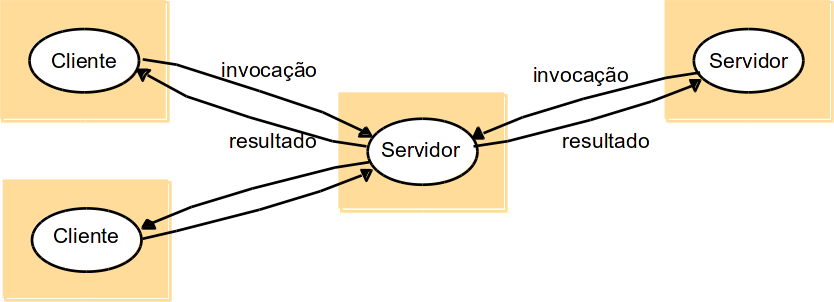
\includegraphics[scale=0.4]{cs2}%% Dimensões e localização
  \fonte{Adaptado de \citeonline{Coulouris2013}}%% Fonte
\end{figure}

Utilizando o pacote \textit{subfig} é possível adicionar figuras lado a lado, como pode ser observado na \autoref{fig:exemplo2}.

\begin{figure}[htb]
  \caption{Telas de cadastro de Paciente: (a) Cadastro Paciente, (b) Cadastro Paciente 2}
  \label{fig:exemplo2}
  \centering
  \subfloat[Cadastro Paciente]{
    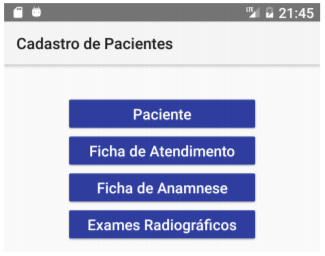
\includegraphics[scale=0.7]{cadastro-paciente}
  }\hspace{0.15cm}
  \subfloat[Cadastro Paciente 2]{
    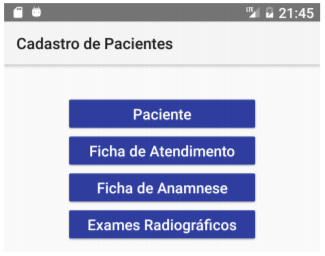
\includegraphics[scale=0.7]{cadastro-paciente}
  }

  \fonte{}
\end{figure}

Este modelo vem com o ambiente \texttt{quadro} e impressão de Lista de quadros
configurados por padrão.  Este parágrafo apresenta como referenciar o quadro no texto, requisito obrigatório da ABNT. Primeira opção, utilizando \texttt{autoref}: Ver o \autoref{quad:exemplo1}. Segunda opção, utilizando  \texttt{ref}: Ver o Quadro \ref{quad:exemplo1}.

\begin{tabframed}[htb]%% Ambiente tabframed
  %\captionsetup{width=0.5\textwidth}%% Largura da legenda
  \caption{Materiais utilizados no desenvolvimento do sistema}%% Legenda
  \label{quad:exemplo1}%% Rótulo
  \renewcommand{\arraystretch}{1.5}
  \begin{tabular}{|l|l|l|l|l}
    \cline{1-4}
    \textbf{Ferramenta/Tecnologia} & \textbf{Versão} & \textbf{Disponível em} & \textbf{Finalidade}   \\ \cline{1-4}
    Teste                          & 1.0             & https:/teste.org       & Biblioteca de Teste & \\ \cline{1-4}
    Teste                          & 1.0             & https:/teste.org       & Biblioteca de Teste & \\ \cline{1-4}
    Teste                          & 1.0             & https:/teste.org       & Biblioteca de Teste & \\ \cline{1-4}
    Teste                          & 1.0             & https:/teste.org       & Biblioteca de Teste & \\ \cline{1-4}
  \end{tabular}
  \fonte{}%% Fonte
\end{tabframed}


Também é possível citar tabelas no texto. Primeira opção, utilizando \texttt{autoref}: Ver o \autoref{tab:exemplo1}. Segunda opção, utilizando  \texttt{ref}: Ver a Tabela \ref{tab:exemplo1}.

\begin{table}[htb]
  % Luiz - O texto do caption da tabela/quadro deve ser do tamanho da tabela, então utilize a linha a seguir para conseguir esse efeito
  \captionsetup{width=0.33\textwidth}
  \centering
  \caption{\label{tab:exemplo1}Exemplo de tabela com uma legenda contendo um texto longo}
  \begin{tabular}{cccc}
    \hline
    \textbf{Pessoa} & \textbf{Idade} & \textbf{Peso} & \textbf{Altura} \\ \hline
    Marcos          & 26             & 68            & 178             \\
    Ivone           & 22             & 57            & 162             \\
    ...             & ...            & ...           & ...             \\
    Sueli           & 40             & 65            & 153             \\ \hline
  \end{tabular}
  \fonte{}
\end{table}

A \autoref{tab:exemplo2} também pode ser citada no texto.

\begin{table}[htb]%% Ambiente table
  \caption{Segundo exemplo de tabela com uma legenda contendo um texto muito longo que pode ocupar mais de uma linha}%% Legenda
  \label{tab:exemplo2}%% Rótulo
  \begin{tabularx}{\textwidth}{@{\extracolsep{\fill}}llll}%% Ambiente tabularx
    \toprule
    $\bsym{L}$ & $\bsym{L^2}$ & $\bsym{L^3}$ & $\bsym{L^4}$ \\
    \SI{}{[m]} & \SI{}{[m^2]} & \SI{}{[m^3]} & \SI{}{[m^4]} \\ \midrule
    1          & 1            & 1            & 1            \\
    2          & 4            & 8            & 16           \\
    3          & 9            & 27           & 81           \\
    4          & 16           & 64           & 256          \\
    5          & 25           & 125          & 625          \\ \bottomrule
  \end{tabularx}
  \fonte{}%% Fonte
\end{table}

A \autoref{tab:exemplo3} é um exemplo de tabela que ocupa mais de uma página e que foi construída pelo \gls{latex}\index{LaTeX@\latex} utilizando o pacote \texttt{longtable}.

\begin{longtable}{@{\extracolsep{\fill}}lll}%% Ambiente longtable
  \caption{Possíveis tríplices para grade altamente variável\label{tab:exemplo3}}                        \\%% Legenda e rótulo
  \toprule
  \textbf{Tempo (s)} & \textbf{Tríplice escolhida} & \textbf{Outras possíveis tríplices}                 \\
  \midrule
  \endfirsthead%% Encerra cabeçalho da primeira página
  \caption[]{Possíveis tríplices para grade altamente variável}                                          \\%% Legenda
  \multicolumn{3}{r}{\textbf{(continuação)}}                                                             \\
  \toprule
  \textbf{Tempo (s)} & \textbf{Tríplice escolhida} & \textbf{Outras possíveis tríplices}                 \\
  \midrule
  \endhead%% Encerra cabeçalho das demais páginas
  \midrule
  \multicolumn{3}{r}{\textbf{(continua)}}                                                                \\
  \endfoot%% Encerra rodapé das demais páginas
  \bottomrule
  \\[-0.5\linha]
  \caption*{\nomefonte: Adaptado de \citet{Smallen2014}}                                                 \\
  \endlastfoot%% Encerra rodapé da última página
  0                  & (1, 11, 13725)              & (1, 12, 10980), (1, 13, 8235), (2, 2, 0), (3, 1, 0) \\
  2745               & (1, 12, 10980)              & (1, 13, 8235), (2, 2, 0), (2, 3, 0), (3, 1, 0)      \\
  5490               & (1, 12, 13725)              & (2, 2, 2745), (2, 3, 0), (3, 1, 0)                  \\
  8235               & (1, 12, 16470)              & (1, 13, 13725), (2, 2, 2745), (2, 3, 0), (3, 1, 0)  \\
  10980              & (1, 12, 16470)              & (1, 13, 13725), (2, 2, 2745), (2, 3, 0), (3, 1, 0)  \\
  13725              & (1, 12, 16470)              & (1, 13, 13725), (2, 2, 2745), (2, 3, 0), (3, 1, 0)  \\
  16470              & (1, 13, 16470)              & (2, 2, 2745), (2, 3, 0), (3, 1, 0)                  \\
  19215              & (1, 12, 16470)              & (1, 13, 13725), (2, 2, 2745), (2, 3, 0), (3, 1, 0)  \\
  21960              & (1, 12, 16470)              & (1, 13, 13725), (2, 2, 2745), (2, 3, 0), (3, 1, 0)  \\
  24705              & (1, 12, 16470)              & (1, 13, 13725), (2, 2, 2745), (2, 3, 0), (3, 1, 0)  \\
  27450              & (1, 12, 16470)              & (1, 13, 13725), (2, 2, 2745), (2, 3, 0), (3, 1, 0)  \\
  30195              & (2, 2, 2745)                & (2, 3, 0), (3, 1, 0)                                \\
  32940              & (1, 13, 16470)              & (2, 2, 2745), (2, 3, 0), (3, 1, 0)                  \\
  35685              & (1, 13, 13725)              & (2, 2, 2745), (2, 3, 0), (3, 1, 0)                  \\
  38430              & (1, 13, 10980)              & (2, 2, 2745), (2, 3, 0), (3, 1, 0)                  \\
  41175              & (1, 12, 13725)              & (1, 13, 10980), (2, 2, 2745), (2, 3, 0), (3, 1, 0)  \\
  43920              & (1, 13, 10980)              & (2, 2, 2745), (2, 3, 0), (3, 1, 0)                  \\
  46665              & (2, 2, 2745)                & (2, 3, 0), (3, 1, 0)                                \\
  49410              & (2, 2, 2745)                & (2, 3, 0), (3, 1, 0)                                \\
  52155              & (1, 12, 16470)              & (1, 13, 13725), (2, 2, 2745), (2, 3, 0), (3, 1, 0)  \\
  54900              & (1, 13, 13725)              & (2, 2, 2745), (2, 3, 0), (3, 1, 0)                  \\
  57645              & (1, 13, 13725)              & (2, 2, 2745), (2, 3, 0), (3, 1, 0)                  \\
  60390              & (1, 12, 13725)              & (2, 2, 2745), (2, 3, 0), (3, 1, 0)                  \\
  63135              & (1, 13, 16470)              & (2, 2, 2745), (2, 3, 0), (3, 1, 0)                  \\
  65880              & (1, 13, 16470)              & (2, 2, 2745), (2, 3, 0), (3, 1, 0)                  \\
  68625              & (2, 2, 2745)                & (2, 3, 0), (3, 1, 0)                                \\
  71370              & (1, 13, 13725)              & (2, 2, 2745), (2, 3, 0), (3, 1, 0)                  \\
  74115              & (1, 12, 13725)              & (2, 2, 2745), (2, 3, 0), (3, 1, 0)                  \\
  76860              & (1, 13, 13725)              & (2, 2, 2745), (2, 3, 0), (3, 1, 0)                  \\
  79605              & (1, 13, 13725)              & (2, 2, 2745), (2, 3, 0), (3, 1, 0)                  \\
  82350              & (1, 12, 13725)              & (2, 2, 2745), (2, 3, 0), (3, 1, 0)                  \\
  85095              & (1, 12, 13725)              & (1, 13, 10980), (2, 2, 2745), (2, 3, 0), (3, 1, 0)  \\
  87840              & (1, 13, 16470)              & (2, 2, 2745), (2, 3, 0), (3, 1, 0)                  \\
  90585              & (1, 13, 16470)              & (2, 2, 2745), (2, 3, 0), (3, 1, 0)                  \\
  93330              & (1, 13, 13725)              & (2, 2, 2745), (2, 3, 0), (3, 1, 0)                  \\
  96075              & (1, 13, 16470)              & (2, 2, 2745), (2, 3, 0), (3, 1, 0)                  \\
  98820              & (1, 13, 16470)              & (2, 2, 2745), (2, 3, 0), (3, 1, 0)                  \\
  101565             & (1, 13, 13725)              & (2, 2, 2745), (2, 3, 0), (3, 1, 0)                  \\
  104310             & (1, 13, 16470)              & (2, 2, 2745), (2, 3, 0), (3, 1, 0)                  \\
  107055             & (1, 13, 13725)              & (2, 2, 2745), (2, 3, 0), (3, 1, 0)                  \\
  109800             & (1, 13, 13725)              & (2, 2, 2745), (2, 3, 0), (3, 1, 0)                  \\
  112545             & (1, 12, 16470)              & (1, 13, 13725), (2, 2, 2745), (2, 3, 0), (3, 1, 0)  \\
  115290             & (1, 13, 16470)              & (2, 2, 2745), (2, 3, 0), (3, 1, 0)                  \\
  118035             & (1, 13, 13725)              & (2, 2, 2745), (2, 3, 0), (3, 1, 0)                  \\
  120780             & (1, 13, 16470)              & (2, 2, 2745), (2, 3, 0), (3, 1, 0)                  \\
  123525             & (1, 13, 13725)              & (2, 2, 2745), (2, 3, 0), (3, 1, 0)                  \\
  126270             & (1, 12, 16470)              & (1, 13, 13725), (2, 2, 2745), (2, 3, 0), (3, 1, 0)  \\
  129015             & (2, 2, 2745)                & (2, 3, 0), (3, 1, 0)                                \\
  131760             & (2, 2, 2745)                & (2, 3, 0), (3, 1, 0)                                \\
  134505             & (1, 13, 16470)              & (2, 2, 2745), (2, 3, 0), (3, 1, 0)                  \\
  137250             & (1, 13, 13725)              & (2, 2, 2745), (2, 3, 0), (3, 1, 0)                  \\
  139995             & (2, 2, 2745)                & (2, 3, 0), (3, 1, 0)                                \\
  142740             & (2, 2, 2745)                & (2, 3, 0), (3, 1, 0)                                \\
  145485             & (1, 12, 16470)              & (1, 13, 13725), (2, 2, 2745), (2, 3, 0), (3, 1, 0)  \\
  148230             & (2, 2, 2745)                & (2, 3, 0), (3, 1, 0)                                \\
  150975             & (1, 13, 16470)              & (2, 2, 2745), (2, 3, 0), (3, 1, 0)                  \\
  153720             & (1, 12, 13725)              & (2, 2, 2745), (2, 3, 0), (3, 1, 0)                  \\
  156465             & (1, 13, 13725)              & (2, 2, 2745), (2, 3, 0), (3, 1, 0)                  \\
  159210             & (1, 13, 13725)              & (2, 2, 2745), (2, 3, 0), (3, 1, 0)                  \\
  161955             & (1, 13, 16470)              & (2, 2, 2745), (2, 3, 0), (3, 1, 0)                  \\
  164700             & (1, 13, 13725)              & (2, 2, 2745), (2, 3, 0), (3, 1, 0)                  \\
\end{longtable}


\subsection{Códigos fonte e algoritmos}\label{subsec:algoritimos}

Os algoritmos podem ser utilizados para explicar uma determinada rotina desenvolvida. Conforme pode ser observado no \autoref{alg:exemplo1}.

\begin{algorithm}[htb]%% Ambiente algorithm
  \caption{Algoritmo de exemplo}%% Legenda
  \label{alg:exemplo1}%% Rótulo
  \hrule
  \begin{algorithmic}[1]%% Ambiente algorithmic
    \ENSURE $A, B$
    \STATE $C = A + B$
    \IF{$C < 10$}
    \STATE $C = 2 \ C$
    \ELSE
    \STATE $C = 0,5 \ C$
    \ENDIF
    \PRINT $A, B, C$
  \end{algorithmic}
  \hrule
  \fonte{}%% Fonte
\end{algorithm}

\lipsum[1]

\lipsum[1]

Na \autoref{code:exemplo1} pode ser visualizado um exemplo de código fonte.

\begin{sourcecode}[htb]
  \caption{\label{code:exemplo1}Exemplo de código}
  \begin{lstlisting}[frame=single, language=Java]
@Entity
public class Foo {
 
    @Id
    @GeneratedValue(strategy = GenerationType.IDENTITY)
    private Long id;
 
    private String name;
    // constructor, getters and setters
}
\end{lstlisting}
  \fonte{}
\end{sourcecode}

%% Comente para remover este item

%% Capítulo
% % ATENÇÃO - veja com o seu orientador se você vai ter este capítulo e se este vai ter nome!
\chapter{Trabalhos Relacionados}
\label{cap:trabalhos:relacionados}

Apresente aqui os trabalhos similares ao seu trabalho ou que são importantes para o entendimento do seu trabalho...

(ATENÇÃO - )
\caixa{Atenção}{Veja com o seu orientador se você vai ter este capítulo e se este vai ter nome, talvez ele seja uma seção de outro capítulo...}


TEXTO TEXTO TEXTO TEXTO TEXTO TEXTO TEXTO TEXTO TEXTO TEXTO TEXTO TEXTO TEXTO TEXTO TEXTO TEXTO TEXTO TEXTO TEXTO TEXTO TEXTO TEXTO TEXTO TEXTO TEXTO TEXTO TEXTO TEXTO TEXTO TEXTO TEXTO TEXTO TEXTO TEXTO TEXTO TEXTO TEXTO TEXTO TEXTO TEXTO TEXTO TEXTO TEXTO TEXTO TEXTO TEXTO TEXTO TEXTO TEXTO TEXTO TEXTO TEXTO TEXTO TEXTO TEXTO TEXTO TEXTO TEXTO TEXTO TEXTO TEXTO TEXTO TEXTO TEXTO TEXTO TEXTO TEXTO TEXTO TEXTO TEXTO TEXTO TEXTO TEXTO TEXTO TEXTO TEXTO TEXTO TEXTO TEXTO TEXTO TEXTO TEXTO TEXTO TEXTO TEXTO TEXTO TEXTO TEXTO TEXTO TEXTO TEXTO TEXTO TEXTO TEXTO TEXTO TEXTO TEXTO TEXTO TEXTO TEXTO TEXTO TEXTO TEXTO TEXTO TEXTO TEXTO TEXTO TEXTO TEXTO TEXTO TEXTO TEXTO TEXTO TEXTO TEXTO TEXTO TEXTO TEXTO TEXTO TEXTO TEXTO TEXTO TEXTO TEXTO TEXTO TEXTO TEXTO TEXTO TEXTO TEXTO TEXTO TEXTO

%---------------------------------------------------%

%% Comente para remover este item

%% Capítulo
% \include{./capitulos/cap-proposta}%% Comente para remover este item

%% Capítulo
%%%% CAPÍTULO 3 - MATERIAL E MÉTODOS (PODE SER OUTRO TÍTULO DE ACORDO COM O TRABALHO REALIZADO)

\chapter{Materiais e Método}\label{cap:materialemetodos}

A ênfase deste capítulo está em reportar o que e como será feito para alcançar o objetivo do trabalho. Este capítulo pode ser subdividido, inicialmente, em duas seções, sendo uma para os materiais e outra para os métodos.

\section{Materiais}\label{sec:materiais}

Materiais são as ferramentas, as tecnologias, os ambientes de desenvolvimento e outros que são utilizados para realizar as atividades desde a definição dos requisitos à implantação do sistema. Exemplos de materiais: linguagens de programação e de modelagem, banco de dados e seus gerenciadores, editores para análise e modelagem, ambiente e plataforma de desenvolvimento.

Cada um dos materiais pode ter uma subseção própria ou serem descritos em uma mesma seção. De qualquer forma, essa seção não precisa ser muito extensa, deve abranger apenas um conhecimento básico sobre cada um dos materiais e o que é mais relevante ou utilizado para o trabalho proposto. De maneira geral, não há necessidade de incluir informações históricas sobre os materiais. Centrar-se nos conceitos e particularidades mais relevantes para o trabalho. Exceto se necessário para o entendimento do objeto do trabalho ou considerado relevante para o tipo de pesquisa.

\section{Método}\label{sec:metodo}

Os métodos definem, de certa maneira, um plano geral do trabalho, com as principais atividades realizadas durante seu processo de desenvolvimento. São apenas as atividades, o que será feito e o que se espera obter com as mesmas. O que é obtido com a realização dessas atividades está no \autoref{cap:resultados}. 

Os métodos são, basicamente, uma sequência de atividades realizadas para definir o sistema, modelar o problema e a solução, implementar a solução, testar e implantar essa solução. Essas atividades devem enfatizar a forma de uso dos materiais de acordo com o referencial teórico e como foi procedido no sentido de alcançar os objetivos do trabalho.
Os métodos incluem os procedimentos utilizados para se alcançar o objetivo do trabalho. Assim, ele abrange o ciclo de vida do sistema, da identificação do problema à implantação da solução. A identificação pode incluir a definição dos requisitos por parte do usuário e/ou cliente definindo a proposta do sistema. A implantação pode incluir a forma de gerar os instaladores, os recursos e forma de instalação do sistema, a forma de manutenção e de descontinuidade do sistema.

A definição das atividades, passos, ou procedimentos que compõem os métodos podem (ou mesmo deve) estarem baseados em autores. Esses autores, normalmente, estão relacionados à engenharia de software.

O tempo verbal a ser utilizado na descrição dos métodos é o passado, considerando que trata-se de métodos que foram aplicados para a obtenção dos resultados a serem apresentados.
%% Comente para remover este item

%% Capítulo
%%%% CAPÍTULO 4 - RESULTADOS E DISCUSSÃO

\chapter{Resultados}\label{cap:resultados}

Este capítulo descreve os resultados do trabalho, que é um \textit{client web}, com foco no controle de gestão de propriedades rurais, acompanhamento de animais nas propriedades rurais e gerenciamento financeiro da propriedade, entre outras funcionalidades. 

Inicialmente, será apresentado o escopo, destacando as principais funcionalidades e os atores envolvidos. Em seguida, abordaremos a modelagem do sistema, que compreende a definição dos requisitos funcionais e não funcionais, juntamente com a elaboração dos diagramas de casos de uso e do modelo de entidade e relacionamento do banco de dados.

\section{Escopo do sistema}\label{sec:escopoSistema}

O \textit{client web} para gerenciamento de gado leiteiro será principalmente utilizado por técnicos do \gls{IDR-PR}. Sendo a principal finalidade o controle e manuseio dos dados, a fim de evitar incoerência nos registros coletados. A plataforma \textit{front-end web} consumirá dados de uma \gls{API} \gls{REST} que está em desenvolvimento e manutenção em paralelo ao desenvolvimento deste trabalho.

Cada técnico poderá fazer o gerenciamento dos dados da propriedade vinculado, bem como dados do rebanho, dados financeiros, dados de insumos e produtos e dados de plantações.

O sistema iniciará com uma página de autenticação, caso o técnico ainda não possua cadastro ele poderá cadastrar-se. Vale ressaltar que uma propriedade pode ser relacionada a um ou mais técnicos, os técnicos só poderão analisar dados das propriedades em que estão vinculados. Estão incluídos no sistema além de cadastro e autenticação do técnico, o módulo de propriedades, módulo financeiro, módulo de animais, produtos e insumos e o módulo de plantações, sendo que exceto o módulo de propriedade, os demais são sempre referentes a uma propriedade.

No módulo dedicado às propriedades, serão cadastrados diversos dados importantes, incluindo informações sobre o produtor, colaboradores, a área destinada à bovinocultura (em hectares), coordenadas de localização e uma imagem representativa da propriedade.

Na seção voltada aos animais, serão registradas informações abrangentes, tais como dados sobre partos, inseminações, casos de mastite, doenças, medicamentos administrados, diagnósticos de prenhez, além de detalhes sobre vendas, compras e óbitos de animais.

No módulo relacionado às plantações, haverá um controle rigoroso sobre informações envolvendo pragas e doenças, abrangendo a identificação da cultura afetada, o tipo de praga ou doença identificada e o grau de infestação presente.

No que concerne ao módulo financeiro, serão meticulosamente gerenciados registros de receitas e despesas. Tais registros incluirão datas, tipos, quantidades, valores expressos em reais e descrições detalhadas, com a possibilidade de realizar agrupamentos para uma análise mais precisa.

No módulo de produtos e insumos, os usuários terão a capacidade de controlar detalhes referentes aos produtos utilizados, quantidade empregada, data de aplicação e o propósito da utilização específica.

Dessa maneira, todas as informações referentes à uma propriedade rural serão armazenadas e servirão como subsídio para que os técnicos possam auxiliar na melhora da produtividade dessas propriedades.


\section{Modelagem do sistema}\label{sec:modelagemSistema}

A modelagem do sistema inclui os diagramas e as descrições textuais para representar o problema e a solução.

Sendo assim, primeiramente esse item deve apresentar diagramas utilizados para a modelagem de negócios (ex. diagramas de atividade e estado), se esses tenham sido necessários.
Em seguida esse item deve conter a descrição dos requisitos obtidos do usuário, contendo sua respectiva classificação (funcionais e não funcionais). Sugere-se o uso de um modelo formal sugerido por autores (ex. Wazlawick, Bezerra) para a apresentação dessa classificação.

Se utilizada orientação a objetos e a UML, nesta seção ainda são apresentados, por exemplo, os diagramas de casos de uso, com suas descrições suplementares, os diagramas de classe de análise (ou modelo conceitual), de sequência e/ou comunicação, diagrama de classes de projeto.

Nesta seção também estão os diagramas da modelagem de banco de dados, como entidade-relacionamento. Nesse item pode ser apresentada a descrição de cada uma das classes do modelo de classes apresentado acima, assim como a descrição das tabelas do banco de dados. Também podem estar documentados modelos e padronizações utilizados para a interface, diagramas de navegação, a representação da arquitetura do sistema e dos padrões de projeto utilizados.

\section{Apresentação do sistema}\label{sec:apresentacaoSistema}

Apresenta as funcionalidades e o uso de recursos tecnológicos do sistema por meio de suas telas, enfatizando a interação com o sistema. A apresentação do sistema é feita sob a forma de texto, com telas e definição de padrões que forem relevantes ao contexto do trabalho. As telas são tratadas como figuras, cópias (print screen) de relatórios ou consultas também são figuras.

A \autoref{fig:cadastroPaciente} exibe a tela de acesso ao Cadastro de Pacientes.

\begin{figure}[htpb]%% Ambiente figure
  \captionsetup{width=0.43\textwidth}
  \caption{Tela de acesso ao Cadastro de Pacientes.}%% Legenda
  \label{fig:cadastroPaciente}%% Rótulo
  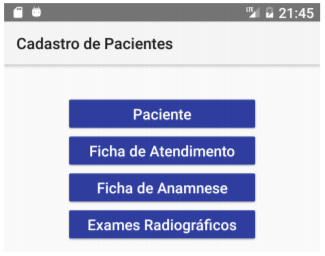
\includegraphics[scale=0.8]{cadastro-paciente}%% Dimensões e localização
  \fonte{}%% Fonte
\end{figure}

\section{Implementação do sistema}\label{sec:implementacaoSistema}

Nesta seção é documentada a implementação do sistema com partes relevantes ou exemplos de código, rotinas, funções. Inclui, ainda, a descrição técnica do uso de recursos (componentes, bibliotecas, etc.) da linguagem. Ressalta-se que cada orientador avaliará juntamente com seu orientado o que poderá ser descrito nesta seção. Isso sem que sejam revelados detalhes do sistema que possam comprometer seu uso comercial ou científico ou que a descrição fique muito sucinta ou superficial.

Em materiais e método estão quais os recursos utilizados, neste capítulo é reportado como esses recursos foram utilizados para resolver o problema.

Sugere-se colocar listagens curtas de código, enfatizando aspectos específicos das tecnologias utilizadas ou da implementação. Sugere-se, ainda, que o código não seja apresentado sob a forma de print screen, e sim copiado e colado no texto, mantendo, se possível, a formatação. Todas as listagens de código devem ser devidamente explicadas. A explicação deve ser técnica, fundamentada em aspectos conceituais e boas práticas de programação.

Enfatizar os diferenciais do sistema: procedimentos armazenados, consultas SQL, uso de componentes, uso de padrões de projeto, a forma de uso dos recursos da linguagem. Esses diferenciais são no sentido de explicitar as vantagens, desvantagens, dificuldades e facilidades que esses recursos impetraram no desenvolvimento do sistema em termos técnicos. Esses diferenciais servirão para avaliar pela utilização ou não desses recursos, pelo menos para sistemas iguais ou semelhantes ao reportado no trabalho.

Reportar a forma como o sistema foi verificado e validado. No sentido de verificar se os requisitos definidos para o mesmo foram atendidos. Os testes podem ser realizados pelo professor orientador, pelos professores que compõem a banca, por pessoas que serviram de base para as informações para o sistema e etc. Os testes podem ser realizados com base em um plano de testes elaborado juntamente com a análise e projeto do sistema. Para validar a implementação podem ser desenvolvidas rotinas de teste unitário.

Se houver implantação do sistema, mesmo que seja para teste, reportar a forma como isso foi feito, a geração de instaladores, os problemas com ambiente e sistema operacional, incluindo banco de dados e outros. Deixar explícito o procedimento para instalar e usar o sistema.

Quando for necessário, citar no texto do trabalho nomes de campos, tabelas ou rotinas específicas utilizadas na implementação de um software, utilizar a fonte courier new para destacar esses nomes.

Um exemplo de listagem de código fonte pode ser observado na \autoref{codigo:classeFoo}, que representa a classe Aluno.

\begin{sourcecode}[htb]
  \caption{\label{codigo:classeFoo}Classe Aluno}
  \begin{lstlisting}[frame=single, language=Java]
@Entity
public class Foo {
 
    @Id
    @GeneratedValue(strategy = GenerationType.IDENTITY)
    private Long id;
 
    private String nome;
    
    private Integer ra;
     
    // constructor, getters and setters
}
\end{lstlisting}
  \fonte{}
\end{sourcecode}

\section{Discussões (opcional)}\label{sec:discussoes}

O trabalho contém esta seção quando considerado que há resultados (em termos de dados) e discussões relevantes ou suficientes para justificar uma seção. Se existentes e não justificarem uma seção, eles podem estar na seção que relata a implementação do sistema.

Nesta seção estão os resultados obtidos da realização de testes quantitativos e qualitativos, independentemente da quantidade, tipo e volume de testes realizados. Os resultados dos testes são discutidos tendo como base o referencial teórico e os objetivos pretendidos com o trabalho. Esses testes podem resultar de implantação e testes de uso do sistema.
%% Comente para remover este item

%% Capítulo - esse capítulo contém exemplos para melhor uso do modelo Latex
%% Na versão final do TCC esse capítulo deve ser removido utilizando o sinal %
%%%%% CAPÍTULO - EXEMPLO
%%
%% Capítulo de informações e exemplos de utilização deste modelo.

%% Título e rótulo de capítulo (rótulos não devem conter caracteres especiais, acentuados ou cedilha)
\chapter{Informações e Exemplos de Utilização deste Modelo}\label{cap:exemplo}

Devido à necessidade de padronização em trabalhos acadêmicos (teses, dissertações, trabalhos de conclusão de curso, etc.), são utilizadas neste documento algumas regras básicas para estruturação e formatação.

O presente documento/\textit{template} foi produzido em parceria entre a \gls{utfpr} de Pato Branco e a \gls{utfpr} de Campo Mourão. Assim, derivado do \gls{utfprpbtex}\index{UTFPRPBTeX@\utfprpbtex} e de alterações implementadas pela UTFPR de Campo Mourão, surge o \utfprtex, como um proposta de um modelo \latex que pode ser utilizado por qualquer campus da \gls{utfpr} para elaboração de trabalhos acadêmicos segundo as normas definidas pela \gls{abnt}\index{ABNT}. Este modelo foi desenvolvido em linguagem de editoração \gls{tex}\index{TeX@\TeX}/\gls{latex}\index{LaTeX@\latex} com base no modelo \gls{abntex2}\index{abnTeX2@\abnTeX} \cite{abnTeX2:2013}, que atende os requisitos das normas da ABNT para elaboração de documentos técnicos e científicos brasileiros.

Os principais arquivos do modelo são: 
\begin{itemize}
    \item \texttt{main.tex} - é o arquivo principal que relaciona todos os outros arquivos, neste você pode remover ou adicionar elementos textuais (capítulos, etc);
    \item \texttt{configuracoes.tex} - contém os pacotes a serem utilizados pelo ambiente, bem como a criação de comandos do \latex;
    \item \texttt{variaveis.tex} - contém variáveis, como nome do autor, orientador, título, banca e que devem ser alterados para atender cada trabalho;
    \item \texttt{main.bib} - contém as referências bibliográficas;
    \item \texttt{readme.md} - são informações a respeito do template \latex;
    \item \texttt{utfpr.cls} - mantém a formatação do texto - \textbf{não altere esse arquivo a menos que você saiba o que está fazendo}.
\end{itemize}

Além dos arquivos, o \textit{template} contém diretórios/pastas, para ajudar a organizar o trabalho, sendo essas:
\begin{itemize}%% Lista de itens
\item \texttt{PreTexto} - contém arquivos, com nomes auto descritivos, que representam elementos pré textuais como:  resumo, abstract, agradecimentos, siglas, epigrafe, etc;
\item \texttt{capitulos} -  contém arquivos, com nomes auto descritivos, que representam os capítulos do texto, como por exemplo: introdução, metodologia, conclusão, etc. Para adicionar ou remover um capítulo é necessário alterar o arquivo \texttt{main.tex} - ver exemplos no próprio arquivo;
\item \texttt{figuras}  - contém as figuras/imagens utilizadas no texto;
\item \texttt{PosTexto} - contém elementos pós textuais como: anexo, apêndice, etc.
\end{itemize}

A codificação de caracteres em todos os arquivos é \texttt{UTF8}, tanto no modelo \gls{abntex2}\index{abnTeX2@\abnTeX} quanto no modelo \gls{utfprpbtex}\index{UTFPRPBTeX@\utfprtex}. Portanto, é necessário que seja utilizada a mesma codificação nos documentos a serem desenvolvidos, inclusive nos arquivos de base bibliográfica. Diversos editores de arquivos fonte do \gls{latex}\index{LaTeX@\latex} são capazes de manipular e/ou converter entre diferentes codificações, por exemplo, o ``Texmaker\index{Texmaker}'' (disponível em \url{http://www.xm1math.net/texmaker/}). 
%Recomenda-se, sempre que for manipular e/ou substituir um dos arquivos constituintes deste modelo, manter uma cópia do original num local seguro e/ou renomear esta cópia do original para que possa ser utilizada como um exemplo no desenvolvimento do seu próprio arquivo. Por exemplo, quando for criar o seu ``Capítulo 1'', fazer uma cópia do arquivo original \texttt{capitulo1.tex}, renomeando-o para \texttt{capitulo1.original.tex}, por exemplo, e realizar as alterações e/ou modificações no arquivo \texttt{capitulo1.tex}.

Este capítulo\label{errata:capitulo} de exemplo tem por finalidade a definição e a apresentação de alguns comandos do \gls{latex}\index{LaTeX@\latex} e/ou dos modelos \gls{abntex2}\index{abnTeX2@\abnTeX} e \gls{utfprpbtex}\index{UTFPRPBTeX@\utfprtex}. O presente documento não se constitui um manual, tampouco uma apostila de \gls{latex}\index{LaTeX@\latex}, visto que existe uma grande quantidade de material de referência disponível na Internet, como por exemplo em \url{http://en.wikibooks.org/wiki/LaTeX}.

Os capítulos devem conter uma introdução e um fecho. A introdução fornece ao leitor uma breve descrição do que será tratado no capítulo, enquanto o fecho apresenta comentários finais sobre o que foi desenvolvido no capítulo. Os capítulos podem ser divididos em seções\label{errata:secao}. Esta divisão deve ser lógica (temática) e não física (por tamanho). O número ideal de seções é impossível de se precisar. Entretanto, um capítulo com uma única seção, possivelmente, deverá ser agregado ao capítulo anterior ou posterior. Um capítulo com quinze seções, possivelmente, deverá ser subdividido em dois capítulos. Capítulos, seções e subseções\label{errata:subsecao} devem ser rotulados para que possam ser referenciados em qualquer parte do texto. Exemplo: O \autoref{cap:exemplo} é gerado, rotulado e referenciado pelos comandos \verb|\chapter{Informações e...}|, \verb|\label{cap:exemplo}| e \verb|\autoref{cap:exemplo}|, respectivamente.

%% Título e rótulo de seção (rótulos não devem conter caracteres especiais, acentuados ou cedilha)
\section{Título da seção secundária}\label{sec:secsec}

Seções secundárias são divisões do conteúdo das seções primárias. A \autoref{sec:secsec} é gerada, rotulada e referenciada pelos comandos \verb|\section{Título da Seção Secundária}|, \verb|\label{sec:secsec}| e \verb|\autoref{sec:secsec}|, respectivamente.

%% Título e rótulo de seção (rótulos não devem conter caracteres especiais, acentuados ou cedilha)
\subsection{Título da seção terciária}\label{ssec:secterc}

Seções terciárias são divisões do conteúdo de seções secundárias. A \autoref{ssec:secterc} é gerada, rotulada e referenciada pelos comandos \verb|\subsection{Título da Seção Terciária}|, \verb|\label{ssec:secterc}| e \verb|\autoref{ssec:secterc}|, respectivamente.

%% Título e rótulo de seção (rótulos não devem conter caracteres especiais, acentuados ou cedilha)
\subsubsection{Título da seção quartenária}\label{sssec:secquart}

Seções quartenárias são divisões do conteúdo de seções terciárias. A \autoref{sssec:secquart} é gerada, rotulada e referenciada pelos comandos \verb|\subsubsection{Título da seção quartenária}|, \verb|\label{sssec:secquart}| e \verb|\autoref{sssec:secquart}|, respectivamente.

%% Título e rótulo de seção (rótulos não devem conter caracteres especiais, acentuados ou cedilha)
\section{Exemplo de título de seção secundária com um texto muito longo que pode ocupar mais de uma linha}\label{sec:sectitulolongo}

A \autoref{sec:sectitulolongo} é um exemplo de título de seção secundária com texto muito longo, formatado automaticamente de acordo com \citeonline[subseções 5.2.2 a 5.2.4]{NBR14724:2011} e \citeonline[subseções 3.1 a 3.8]{NBR6024:2012}. Segundo as normas, o título de seção deve estar alinhado à esquerda e a segunda e demais linhas devem iniciar logo abaixo da primeira palavra da primeira linha.

%% Título e rótulo de seção (rótulos não devem conter caracteres especiais, acentuados ou cedilha)
\section{Elementos pré-textuais}\label{sec:elempretext}

Alguns elementos pré-textuais do presente documento são gerados automaticamente pelo \gls{utfprpbtex}\index{UTFPRPBTeX@\utfprtex}. Para adicionar e/ou alterar as informações apresentadas na capa, na folha de rosto %, na ficha catalográfica 
e na folha de aprovação deve-se editar o arquivo \texttt{variaveis.tex}. %Os dados informados neste arquivo também são utilizados para gerar a referência do trabalho na errata, no resumo e no \textit{abstract}.

Para adicionar e/ou alterar o texto da errata, da dedicatória, dos agradecimentos, da epígrafe, do resumo e do \textit{abstract} deve-se editar seus respectivos arquivos presentes no diretório ``PreTexto'': \texttt{errata.tex}, \texttt{dedicatoria.tex}, \texttt{agradecimentos.tex}, \texttt{epigrafe.tex}, \texttt{resumo.tex} e \texttt{abstract.tex}.

As listas de algoritmos, de ilustrações e de tabelas são geradas automaticamente pelo \gls{utfprpbtex}\index{UTFPRPBTeX@\utfprtex}. Os itens destas listas são gerados a medida que forem sendo inseridos no texto do documento. 

A lista de abreviaturas, siglas e acrônimos pode ser gerada automaticamente por meio do arquivo \texttt{entradas-acronimos.tex}, utilizando o pacote \texttt{glossaries}\footnote{Detalhes sobre comandos para geração de abreviaturas, siglas e acrônimos utilizando o pacote \texttt{glossaries} são apresentadas na \autoref{sec:acronimos}.}, ou por meio da edição do arquivo \texttt{lista-acronimos.tex}. A lista de símbolos pode ser gerada automaticamente utilizando o pacote \texttt{nomencl}\footnote{Detalhes sobre comandos para geração de símbolos utilizando o pacote \texttt{nomencl} são apresentadas na \autoref{sec:simbolos}.} ou mediante a edição do arquivo \texttt{lista-simbolos.tex}. Os arquivos citados estão no diretório ``PreTexto''. O sumário é o último elemento pré-textual e também é gerado automaticamente pelo \gls{utfprpbtex}\index{UTFPRPBTeX@\utfprtex}.

%% Título e rótulo de seção (rótulos não devem conter caracteres especiais, acentuados ou cedilha)
\section{Regras gerais de apresentação}\label{sec:regrasgerais}

As regras gerais de apresentação, definidas na sequência, já estão predefinidas no modelo \gls{utfprpbtex}\index{UTFPRPBTeX@\utfprtex}. Algumas destas regras podem ser alteradas, por comandos apropriados do \gls{latex}\index{LaTeX@\latex}, do \gls{abntex2}\index{abnTeX2@\abnTeX} ou do \gls{utfprpbtex}\index{UTFPRPBTeX@\utfprtex}, no preâmbulo do arquivo principal \texttt{configuracoes.tex} ou em outras partes do documento, por exemplo, nos capítulos.

\begin{itemize}%% Lista de itens
\item Configuração das margens: deve-se usar margens superior e esquerda de \SI{3}{cm}; e margens inferior e direita de \SI{2}{cm}; em papel formato A4 ($\SI{21}{cm} \times \SI{29,7}{cm}$);
\item Recomenda-se o uso de fonte tipo Arial ou Times New Roman, tamanho 12 para o texto e tamanho 10 para citações de mais de três linhas, notas de rodapé e legendas dos algoritmos, ilustrações e tabelas;
\item O parágrafo deve aparecer com recuo na primeira linha de \SI{1,5}{cm}, justificado, sem espaçamento anterior ou posterior;
%\item Os elementos como: o resumo, as notas, as referências, as legendas das ilustrações e tabelas, a natureza do trabalho, o objetivo, o nome da instituição a que é submetida e a área de concentração devem ser digitados em espaço simples.
\item A numeração progressiva para as seções do texto deve ser adotada para evidenciar a sistematização do conteúdo do trabalho;
\item Para os títulos das seções não se utilizam pontos, hífen, travessão, ou qualquer sinal após o indicativo de seção ou de título;
\item Para as seções primárias: utiliza-se negrito e caixa alta;
\item Para as seções secundárias: título em negrito, iniciado em letra maiúscula e demais letras minúsculas;
\item Para as seções terciárias: somente a primeira letra do título da seção em
maiúscula;
\item Para as seções quaternárias: título da seção sublinhado, com inicial em letra maiúscula e demais letras minúsculas.
\item No sumário, os títulos das seções devem aparecer exatamente iguais ao que estão contidos no trabalho.
\end{itemize}

\caixa{Atenção}{No \latex é necessário manter os títulos apenas com a primeira letra maiúscula e o restante em minúsculo, o retante é controlado pelo \latex, então não é necessário se preocupar com a formatação!}

Recomenda-se evitar, sempre que possível, o uso dos seguintes recursos (ou enfeites) no documento:

\begin{itemize}%% Lista de itens
\item \textbf{o uso de negrito;}
\item \textit{o uso de itálico (exceto em palavras em outra língua);}
\item \texttt{texto em diferente fonte como máquina de escrever;}
\item \underline{o uso de texto sublinhado;}
\item o uso excessivo de\footnote{Notas de rodapé.}.
\end{itemize}

\noindent Lembre-se: um texto ``limpo'' é mais agradável de ler que um texto ``enfeitado''.

%% Título e rótulo de seção (rótulos não devem conter caracteres especiais, acentuados ou cedilha)
\subsection{Espaçamento}\label{sec:espacamento}

\begin{itemize}%% Lista de itens
%\item O resumo, o \textit{abstract}, as notas, as referências, as legendas das ilustrações e tabelas e a natureza do trabalho devem ser digitadas em espaço simples.
\item Todo o texto deve ser formatado com espaço entre linhas de um fator de 1,5 (sem espaçamento antes/depois).
\item As citações com mais de três linhas devem ser em espaço simples e com recuo de \SI{4}{cm} da margem esquerda.
\item As referências, ao final do trabalho, devem ser separadas entre si por um espaços simples, e na mesma referência o espaço é simples.
%\item Os títulos das seções secundárias devem ser separados do texto que os precede por dois espaços entre linhas de um fator de 1,5.
\item As seções primárias devem iniciar em páginas distintas.
\end{itemize}

O recuo na primeira linha, espaço entre a margem e o início do parágrafo, pode ser redefinido definido pelo comando:

\begin{SingleSpacing}%% Ambiente SingleSpacing
\begin{verbatim}
\setlength{\parindent}{1.5cm}
\end{verbatim}
\end{SingleSpacing}

O espaçamento entre um parágrafo e outro\index{espaçamento!entre os parágrafos} pode ser redefinido pelo comando:

\begin{SingleSpacing}%% Ambiente SingleSpacing
\begin{verbatim}
\setlength{\parskip}{0mm} %% Tente também \onelineskip
\end{verbatim}
\end{SingleSpacing}

O controle do espaçamento entre linhas\index{espaçamento!entre as linhas} pode ser redefinido pelo comando:

\begin{SingleSpacing}%% Ambiente SingleSpacing
\begin{verbatim}
\OnehalfSpacing %% Espaçamento um e meio (padrão)
\DoubleSpacing  %% Espaçamento duplo
\SingleSpacing  %% Espaçamento simples
\end{verbatim}
\end{SingleSpacing}

Para isso, também estão disponíveis os ambientes:

\begin{SingleSpacing}%% Ambiente SingleSpacing
\begin{verbatim}
\begin{SingleSpacing} ...     \end{SingleSpacing}
\begin{Spacing}{<factor>} ... \end{Spacing}
\begin{OnehalfSpacing} ...    \end{OnehalfSpacing}
\begin{OnehalfSpacing*} ...   \end{OnehalfSpacing*}
\begin{DoubleSpacing} ...     \end{DoubleSpacing}
\begin{DoubleSpacing*} ...    \end{DoubleSpacing*}
\end{verbatim}
\end{SingleSpacing}

Para mais informações, consulte \citeonline[p. 47-52 e 135]{Wilson2010}.

\subsection{Exemplo de quantidades de subseções}\label{sec:exSubsec}

Quando um item é dividido, precisa ter pelo menos dois sub-itens (não pode ter apenas um), por exemplo para ter a subseção 4.1 é obrigatório ter pelo menos a subseção 4.2, não pode somente a primeira subseção.

%% Título e rótulo de seção (rótulos não devem conter caracteres especiais, acentuados ou cedilha)
\section{Enumerações: alíneas e subalíneas}\label{sec:enumeracoes}\index{alíneas}\index{subalíneas}

Quando for necessário enumerar os diversos assuntos de uma seção que não possua título, esta deve ser subdividida em alíneas\index{alíneas} \cite[subseção 4.2]{NBR6024:2012}:

\begin{alineas}%% Ambiente alineas
\item os diversos assuntos que não possuam título próprio, dentro de uma mesma seção, devem ser subdivididos em alíneas\index{alíneas};
\item o texto que antecede as alíneas\index{alíneas} termina em dois pontos;
\item as alíneas\index{alíneas} devem ser indicadas alfabeticamente, em letra minúscula, seguida de parêntese. Utilizam-se letras dobradas, quando esgotadas as letras do alfabeto;
\item as letras indicativas das alíneas\index{alíneas} devem apresentar recuo em relação à margem esquerda;
\item o texto da alínea deve começar por letra minúscula e terminar em ponto-e-vírgula, exceto a última alínea que termina em ponto final;
\item o texto da alínea deve terminar em dois pontos, se houver subalínea;
\item a segunda e as seguintes linhas do texto da alínea começa sob a primeira letra do texto da própria alínea;
\item subalíneas\index{subalíneas} \cite[subseção 4.3]{NBR6024:2012} devem ser conforme as alíneas\index{alíneas} a seguir:
\begin{alineas}%% Ambiente alineas
\item as subalíneas\index{subalíneas} devem começar por travessão seguido de espaço;
\item as subalíneas\index{subalíneas} devem apresentar recuo em relação à alínea;
\item o texto da subalínea deve começar por letra minúscula e terminar em ponto-e-vírgula. A última subalínea deve terminar em ponto final, se não houver alínea subsequente;
\item a segunda e as seguintes linhas do texto da subalínea começam sob a primeira letra do texto da própria subalínea.
\end{alineas}
\item no \gls{abntex2}\index{abnTeX2@\abnTeX} estão disponíveis os ambientes \texttt{incisos} e \texttt{subalineas}, que em suma são o mesmo que se criar outro nível de \texttt{alineas}, como nos exemplos à seguir:
\begin{incisos}%% Ambiente incisos
\item \textit{um novo inciso em itálico}\index{incisos}.
\end{incisos}
\item Alínea em \textbf{negrito}:
\begin{subalineas}%% Ambiente subalineas
\item \textit{uma subalínea em itálico};
\item \underline{\textit{uma subalínea em itálico e sublinhado}}.
\end{subalineas}
\item última alínea com \emph{ênfase}.
\end{alineas}

%% Título e rótulo de seção (rótulos não devem conter caracteres especiais, acentuados ou cedilha)
\section{Citações}\label{sec:citacoes}

O \gls{utfprpbtex}\index{UTFPRPBTeX@\utfprtex} está configurado para produzir as citações no texto no estilo alfabético (autor-data), segundo as normas \gls{abnt}\index{ABNT}, por meio dos comandos do \gls{abntex2}\index{abnTeX2@\abnTeX} \cite{abnTeX2:2013Cite,abnTeX2:2013CiteAlf}. A lista dos principais comandos são apresentadas a seguir:

\begin{itemize}%% Lista de itens
\item \verb|\cite{rótulo}| -- para gerar citação implícita. Por exemplo, a citação ``\ldots\ \cite{Thompson2001}\ldots'' é gerada pelo comando \verb|\cite{Thompson2001}| ou pelo atalho \verb|\citep{Thompson2001}|, definido em \texttt{utfprpb.tex}.
\item \verb|\citeonline{rótulo}| -- para gerar citação explícita. Por exemplo a citação ``\ldots\ conforme proposto por \citeonline{Thompson2001}\ldots'' é gerada pelo comando \verb|\citeonline{Thompson2001}| ou pelo atalho \verb|\citet{Thompson2001}|, definido em \texttt{utfprpb.tex}.
\item \verb|(\citeauthor{rótulo})| -- para gerar citação implícita somente do autor. Por exemplo, a citação ``\ldots\ (\citeauthor{Thompson2001})\ldots'' é gerada pelo comando \verb|(\citeauthor{Thompson2001})| ou pelo atalho \verb|\citepa{Thompson2001}|, definido em \texttt{utfprpb.tex}.
\item \verb|\citeauthoronline{rótulo}| -- para gerar citação explícita somente do autor. Por exemplo, a citação ``\ldots\ conforme a relação de \citeauthoronline{Thompson2001}\ldots'' é gerada pelo comando \verb|\citeauthoronline{Thompson2001}| ou pelo atalho \verb|\citeta{Thompson2001}|, definido em \texttt{utfprpb.tex}.
\item \verb|(\citeyear{rótulo})| -- para gerar citação implícita somente do ano. Por exemplo, a citação ``\ldots\ (\citeyear{Thompson2001})\ldots'' é gerada pelo comando \verb|(\citeyear{Thompson2001})| ou pelo atalho \verb|\citepy{Thompson2001}|, definido em \texttt{utfprpb.tex}.
\item \verb|\citeyear{rótulo}| -- para gerar citação explícita somente do ano. Por exemplo, a citação ``\ldots\ no ano de \citeyear{Thompson2001}\ldots'' é gerada pelo comando \verb|\citeyear{Thompson2001}| ou pelo atalho \verb|\citety{Thompson2001}|, definido em \texttt{utfprpb.tex}.
\end{itemize}

Informações sobre a utilização dos comandos listados acima e os demais comandos para geração de referências, utilizados pelo \gls{abntex2}\index{abnTeX2@\abnTeX}, podem ser encontradas em \citeonline{abnTeX2:2013Cite,abnTeX2:2013CiteAlf}, disponíveis em \url{http://www.abntex.net.br/}.

\gls{latex}\index{LaTeX@\latex} utiliza um arquivo externo (em separado) para o banco de dados das referências citadas no texto. Este arquivo é compilado pelo \gls{bibtex}\index{BibTeX@Bib\TeX} e deve possuir a extensão \texttt{bib}, como nos arquivos \texttt{referencias.bib} e \texttt{referencias-modelos.bib} presentes no diretório ``PosTexto'', utilizados neste documento. O arquivo \texttt{referencias-modelos.bib} apresenta exemplos dos seguintes estilos de referência aceitos pelo \gls{bibtex}\index{BibTeX@Bib\TeX}:

\begin{itemize}%% Lista de itens
\item anais de simpósios \citep{Alt1995,Pirmez2002};
\item artigos em anais de simpósios \citep{Faina2001};
\item artigos em coletâneas de artigos \citep{Pinto2000};
\item artigos em revistas \citep{Guimaraes2003};
\item capítulos de livros \citep{Santos2000};
\item livretos \citep{Thompson2001};
\item livros \citep{Pedrycz1998};
\item manuais técnicos \citep{IONA1999};
\item miscelânea \citep{Cruz2003};
\item páginas na Internet \cite[acessado em 1 de janeiro de 2004]{Larsson2003} (utilizar a data do último acesso à página);
\item relatórios técnicos \citep{OMG2000};
\item teses de mestrado \citep{SantosFilho2003};
\item teses de doutorado \citep{Faina2000};
\item trabalhos não publicados \citep{Sichman2002}.
\end{itemize}

\subsection{Programas úteis para citações}\label{sec:progUteisCitacoes}

Existem alguns programas para gerenciamento de banco de dados de referências bibliográficas (arquivos \texttt{bib}) do \gls{bibtex}\index{BibTeX@Bib\TeX}. O ``JabRef'' é um exemplo destes programas e está disponível em: \url{http://jabref.sourceforge.net/}.

%% Título e rótulo de seção (rótulos não devem conter caracteres especiais, acentuados ou cedilha)
\subsection{Citações diretas}\label{sec:citacoesdiretas}\index{citações!diretas}

O ambiente \texttt{citacao} permite a inclusão de citações diretas que ocupam mais de três linhas:

\begin{citacao}%% Ambiente citacao
As citações diretas no texto, que ocupam mais de três linhas, devem ser destacadas com recuo de \SI{4}{cm} da margem esquerda, com letra menor que a do texto utilizado e sem as aspas. No caso de documentos datilografados, deve-se observar apenas o recuo \cite[subseção 5.3]{NBR10520:2002}.
\end{citacao}

\noindent Esta citação direta com mais de três linhas foi gerada da seguinte forma:

\begin{SingleSpacing}%% Ambiente SingleSpacing
\begin{verbatim}
\begin{citacao}
As citações diretas no texto, com mais de três linhas,...
... observar apenas o recuo \cite[subseção 5.3]{NBR10520:2002}.
\end{citacao}
\end{verbatim}
\end{SingleSpacing}

O ambiente \texttt{citacao} pode receber como parâmetro opcional um nome de idioma previamente carregado nas opções da classe (definido no preâmbulo do arquivo \texttt{utfprpb.tex}). Neste caso, o texto da citação é automaticamente escrito em itálico e a hifenização é ajustada para o idioma selecionado na opção do ambiente. Por exemplo:

\begin{SingleSpacing}%% Ambiente SingleSpacing
\begin{verbatim}
\begin{citacao}[english]
Text in English language in italic with correct hyphenation.
\end{citacao}
\end{verbatim}
\end{SingleSpacing}

\noindent Tem como resultado:

\begin{citacao}[english]%% Ambiente citacao
Text in English language in italic with correct hyphenation.
\end{citacao}

Citações simples\index{citações!simples}, com até três linhas, devem ser incluídas com aspas. Observe que em \gls{latex}\index{LaTeX@\latex} as aspas iniciais são diferentes das finais: ``Amor é fogo que arde sem se ver''.

%% Título e rótulo de seção (rótulos não devem conter caracteres especiais, acentuados ou cedilha)
\section{Equações}\label{sec:equacoes}

\gls{latex}\index{LaTeX@\latex} é insuperável no processamento de equações. Equações simples como $y = a x^2 + b x + c$ podem ser adicionadas ao longo do texto ou em uma linha própria:
%
\[%% Ambiente displaymath
y = a x^2 + b x + c
\]

Equações complexas como:
%
\begin{equation}%% Ambiente equation
\label{eq:equation1}%% Rótulo
\begin{array}{lcl}%% Ambiente array
p \left(\gamma\right)
& = &
\frac{1}{2}
\sqrt{\frac{M}{\gamma \bar{\gamma}_b}}
\frac{1}{\prod_{i = 1}^M \sqrt{\tilde{\gamma}_i}}
\int_0^{\sqrt{M \delta}}
\int_0^{\sqrt{M \delta} - r_M} \cdots
\int_0^{\sqrt{M \delta} - \sum_{i = 3}^M r_i} \\[0.5\linha]
& &
p \left(%
\frac{\sqrt{M \delta} - \sum_{i = 2}^M r_i}{\sqrt{\tilde{\gamma}_1}},
\frac{r_2}{\sqrt{\tilde{\gamma}_2}}, \ldots,
\frac{r_M}{\sqrt{\tilde{\gamma}_M}}
\right) \, \der r_2 \cdots \der r_{M - 1} \, \der r_M
\end{array}
\end{equation}

\noindent ou
%
\begin{equation}%% Ambiente equation
\label{eq:equation2}%% Rótulo
T \left(r\right) =
\frac{1}{f_m}
\left(%
\frac{\pi}{2} \sum_{i = 1}^M {\tilde{r}_i^2 \dot{\varsigma}_i^2}
\right)^{-1/2}
\frac{%
\begin{array}{ll}%% Ambiente array
\int_0^{\rho \sqrt{M}}
\int_0^{\rho \sqrt{M} - r_M} \cdots
\int_0^{\rho \sqrt{M} - \sum_{i = 3}^M r_i}
\int_0^{\rho \sqrt{M} - \sum_{i = 2}^M r_i} \\[0.5\linha]
p \left(%
\frac{r_1}{\tilde{r}_1},
\frac{r_2}{\tilde{r}_2}, \ldots,
\frac{r_M}{\tilde{r}_M}
\right) \, \der r_1 \, \der r_2 \cdots \der r_{M - 1} \, \der r_M \\[0.5\linha]
\end{array}
}{%
\begin{array}{ll}%% Ambiente array
\int_0^{\rho \sqrt{M}}
\int_0^{\rho \sqrt{M} - r_M} \cdots
\int_0^{\rho \sqrt{M} - \sum_{i = 3}^M r_i} \\[0.5\linha]
p \left(%
\frac{\rho \sqrt{M} - \sum_{i = 2}^M r_i}{\tilde{r}_1},
\frac{r_2}{\tilde{r}_2}, \ldots,
\frac{r_M}{\tilde{r}_M}
\right) \, \der r_2 \cdots \der r_{M - 1} \, \der r_M \\[0.5\linha]
\end{array}
}
\end{equation}

\noindent são automaticamente numeradas e podem ser referenciadas ao longo do texto. Por exemplo, a \seqref{eq:equation1} é trivialmente derivada da \seqref{eq:equation2}. Veja os exemplos de comandos para estas equações no arquivo fonte deste capítulo.

%% Título e rótulo de seção (rótulos não devem conter caracteres especiais, acentuados ou cedilha)
\section{Algoritmos}\label{sec:algoritmos}

Algoritmos podem ser inseridos por meio do pacote \texttt{algorithms}, conforme exemplos no arquivo fonte deste capítulo e cujos resultados são apresentados no \autoref{alg:algoritmo1} e no \autoref{alg:algoritmo2}.

\begin{algorithm}[htb]%% Ambiente algorithm
\caption{Primeiro exemplo de algoritmo com uma legenda contendo um texto muito longo que pode ocupar mais de uma linha}%% Legenda
\label{alg:algoritmo1}%% Rótulo
\hrule
\begin{algorithmic}[1]%% Ambiente algorithmic
\ENSURE $A, B$
\STATE $C = A + B$
\PRINT $C$
\end{algorithmic}
\hrule
\fonte{}%% Fonte
\end{algorithm}

\begin{algorithm}[htb]%% Ambiente algorithm
\caption{Segundo exemplo de algoritmo}%% Legenda
\label{alg:algoritmo2}%% Rótulo
\hrule
\begin{algorithmic}[1]%% Ambiente algorithmic
\ENSURE $A, B$
\STATE $C = A + B$
\IF{$C < 10$}
\STATE $C = 2 \ C$
\ELSE
\STATE $C = 0,5 \ C$
\ENDIF
\PRINT $A, B, C$
\end{algorithmic}
\hrule
\fonte{}%% Fonte
\end{algorithm}

A documentação sobre o pacote \texttt{algorithms} pode ser encontrada em: \url{http://tug.ctan.org/tex-archive/macros/latex/contrib/algorithms/algorithms.pdf}.

%% Título e rótulo de seção (rótulos não devem conter caracteres especiais, acentuados ou cedilha)
\section{Ilustrações}\label{sec:ilustracoes}

O \gls{utfprpbtex}\index{UTFPRPBTeX@\utfprtex} está configurado para produzir os ambientes para os seguintes tipos de ilustrações: figuras, fotografias, gráficos e quadros. Exemplos de uso destes ambientes podem ser observados no arquivo fonte deste capítulo.

%% Título e rótulo de seção (rótulos não devem conter caracteres especiais, acentuados ou cedilha)
\subsection{Figuras}\label{sec:figuras}

Figuras são criadas e/ou editadas com editores gráficos capazes de exportar a figura em formato \gls{ps} ou, preferencialmente, \gls{eps}. O editor ``xfig'' é adequado para a maioria dos casos, como por exemplo, a \autoref{fig:figura1} que foi editada utilizando o ``xfig''. Outras opções para criação/edição de figuras são o GIMP (\url{http://www.gimp.org/}), ou o ``dia'' (\url{http://dia-installer.de/}), um editor orientado a diagramas (UML, fluxograma, etc.) com capacidade de exportar \gls{eps}, como apresentado por \citet{Larsson2003}.

%\gls{gimp}\index{Gimp}
\begin{figure}[htb]%% Ambiente figure
%\captionsetup{width=0.55\textwidth}%% Largura da legenda
\caption{Exemplo de figura criada a partir de um arquivo}%% Legenda
\label{fig:figura1}%% Rótulo
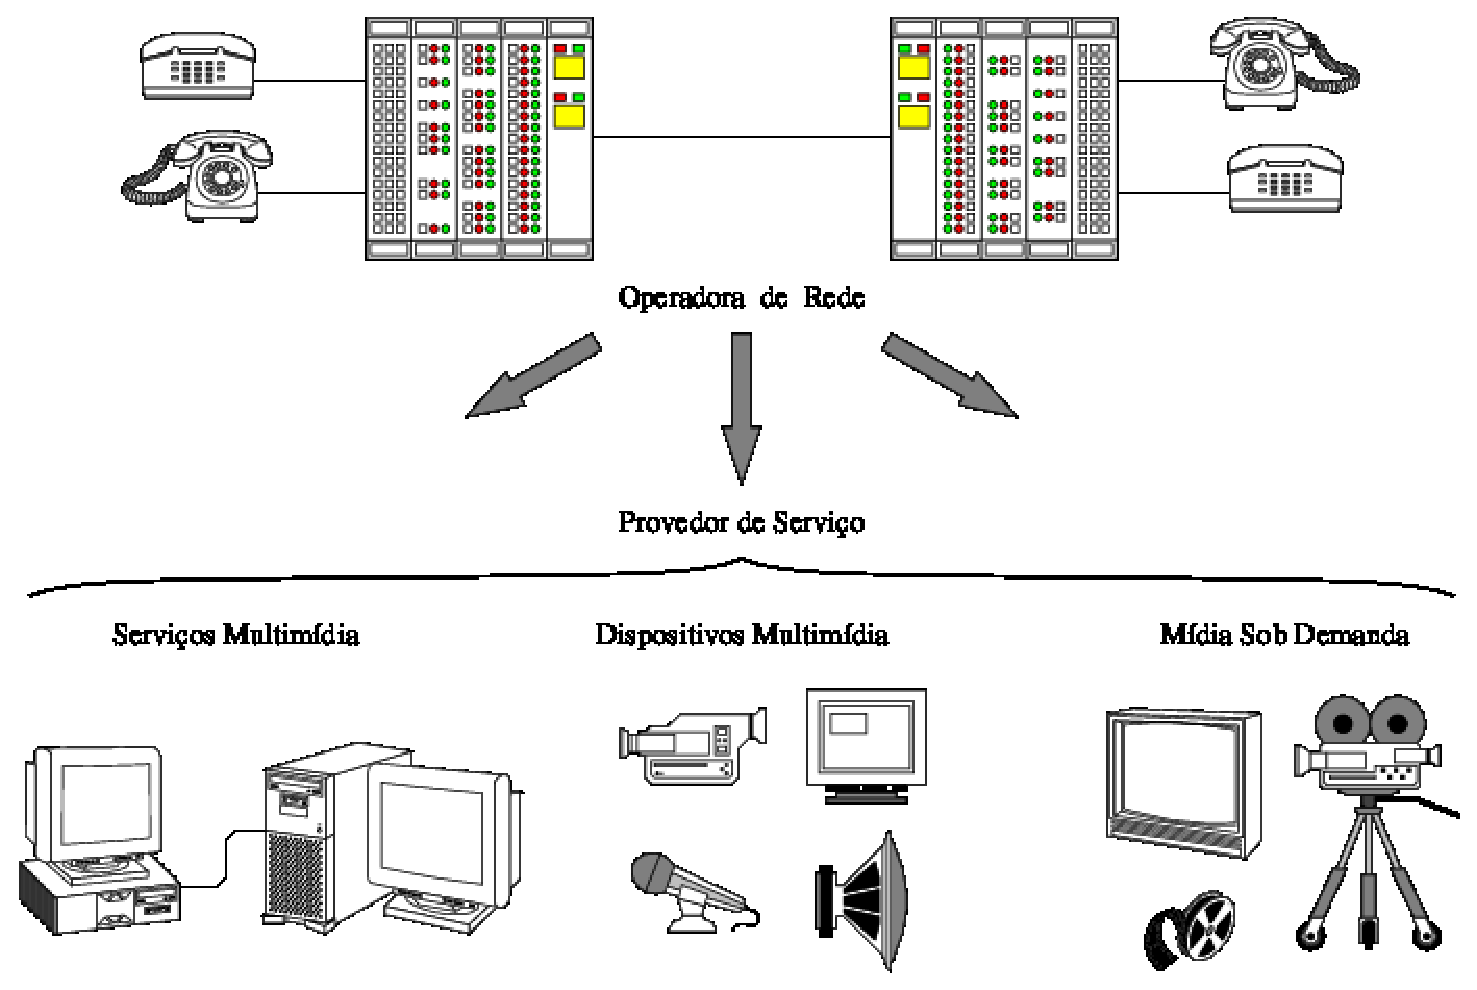
\includegraphics[width=0.6\textwidth]{figura1}%% Dimensões e localização
\fonte{\citet{Larsson2003}}%% Fonte
\end{figure}

Figuras em formato GIF, JPEG e BMP podem ser convertidas para o formato \gls{eps} por meio do aplicativo ``xv''. O ``xv'' não lista o formato \gls{eps} dentre aqueles que é capaz de manipular. Entretanto, selecionando-se o formato \textit{PostScript} e fornecendo-se a extensão \texttt{eps} ao nome do arquivo, o formato \gls{eps} é gerado.

O ambiente \texttt{picture} permite a programação de imagens diretamente no \gls{latex}\index{LaTeX@\latex}, conforme exemplo apresentado na \autoref{fig:figura2}.

\begin{figure}[htb]%% Ambiente figure
%\captionsetup{width=8cm}%% Largura da legenda
\caption{Exemplo de figura criada a partir do ambiente \texttt{picture}}%% Legenda
\label{fig:figura2}%% Rótulo
\setlength{\unitlength}{1cm}%% Unidade de comprimento
\begin{picture}(8,5)(-4,-2.5)%% Ambiente picture
\put(-4,0){\vector(1,0){8}}
\put(3.75,-0.25){$\chi$}
\put(0,-2.5){\vector(0,1){5}}
\multiput(-4,1)(0.4,0){20}{\line(1,0){0.2}}
\multiput(-4,-1)(0.4,0){20}{\line(1,0){0.2}}
\put(0.25,2.25){$\beta \equiv v / c = \tanh \chi$}
\qbezier(0,0)(0.8853,0.8853)(2,0.9640)
\qbezier(0,0)(-0.8853,-0.8853)(-2,-0.9640)
\end{picture}
\fonte{}%% Fonte
\end{figure}

%% Título e rótulo de seção (rótulos não devem conter caracteres especiais, acentuados ou cedilha)
\subsection{Fotografias}\label{sec:fotografias}

Um exemplo deste tipo de ilustração é apresentado na \autoref{foto:foto1}.

\begin{photograph}[htb]%% Ambiente photograph
%\captionsetup{width=0.6\textwidth}%% Largura da legenda
\caption{Camaleão pantera fotografado por Joel Sartore, National Geographic}%% Legenda
\label{foto:foto1}%% Rótulo
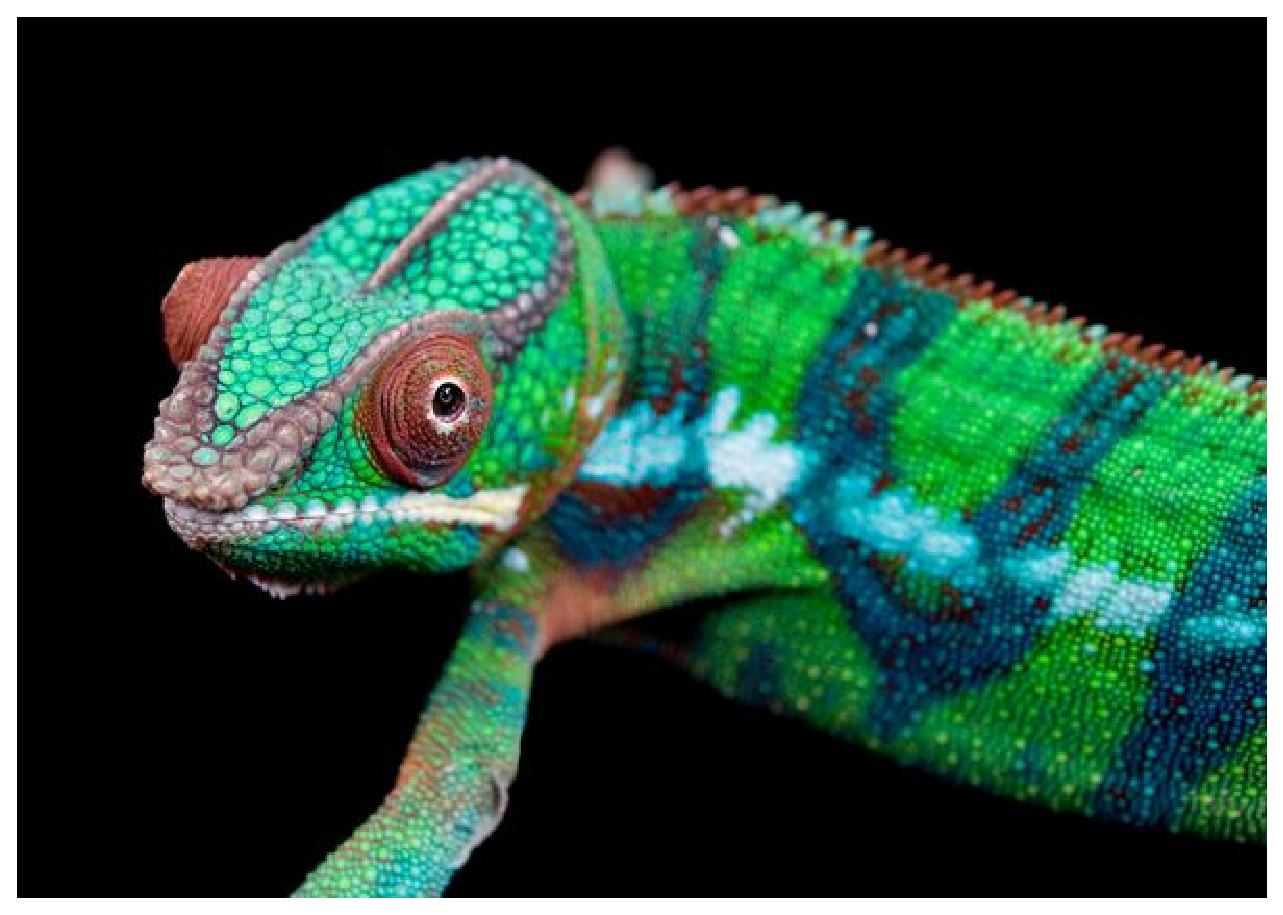
\includegraphics[width=0.95\textwidth]{foto1}%% Dimensões e localização
\fonte{\citet{Sartore2013}}%% Fonte
\end{photograph}

Outro exemplo deste tipo de ilustração é apresentado na \autoref{foto:foto2}.

\begin{photograph}[htb]%% Ambiente photograph
\captionsetup{width=0.6\textwidth}%% Largura da legenda
\caption{Fotografia da erupção vulcânica em 1982 do Galungung, Indonésia (com descargas de raios), produzida pelo Serviço Geológico dos Estados Unidos da América}%% Legenda
\label{foto:foto2}%% Rótulo
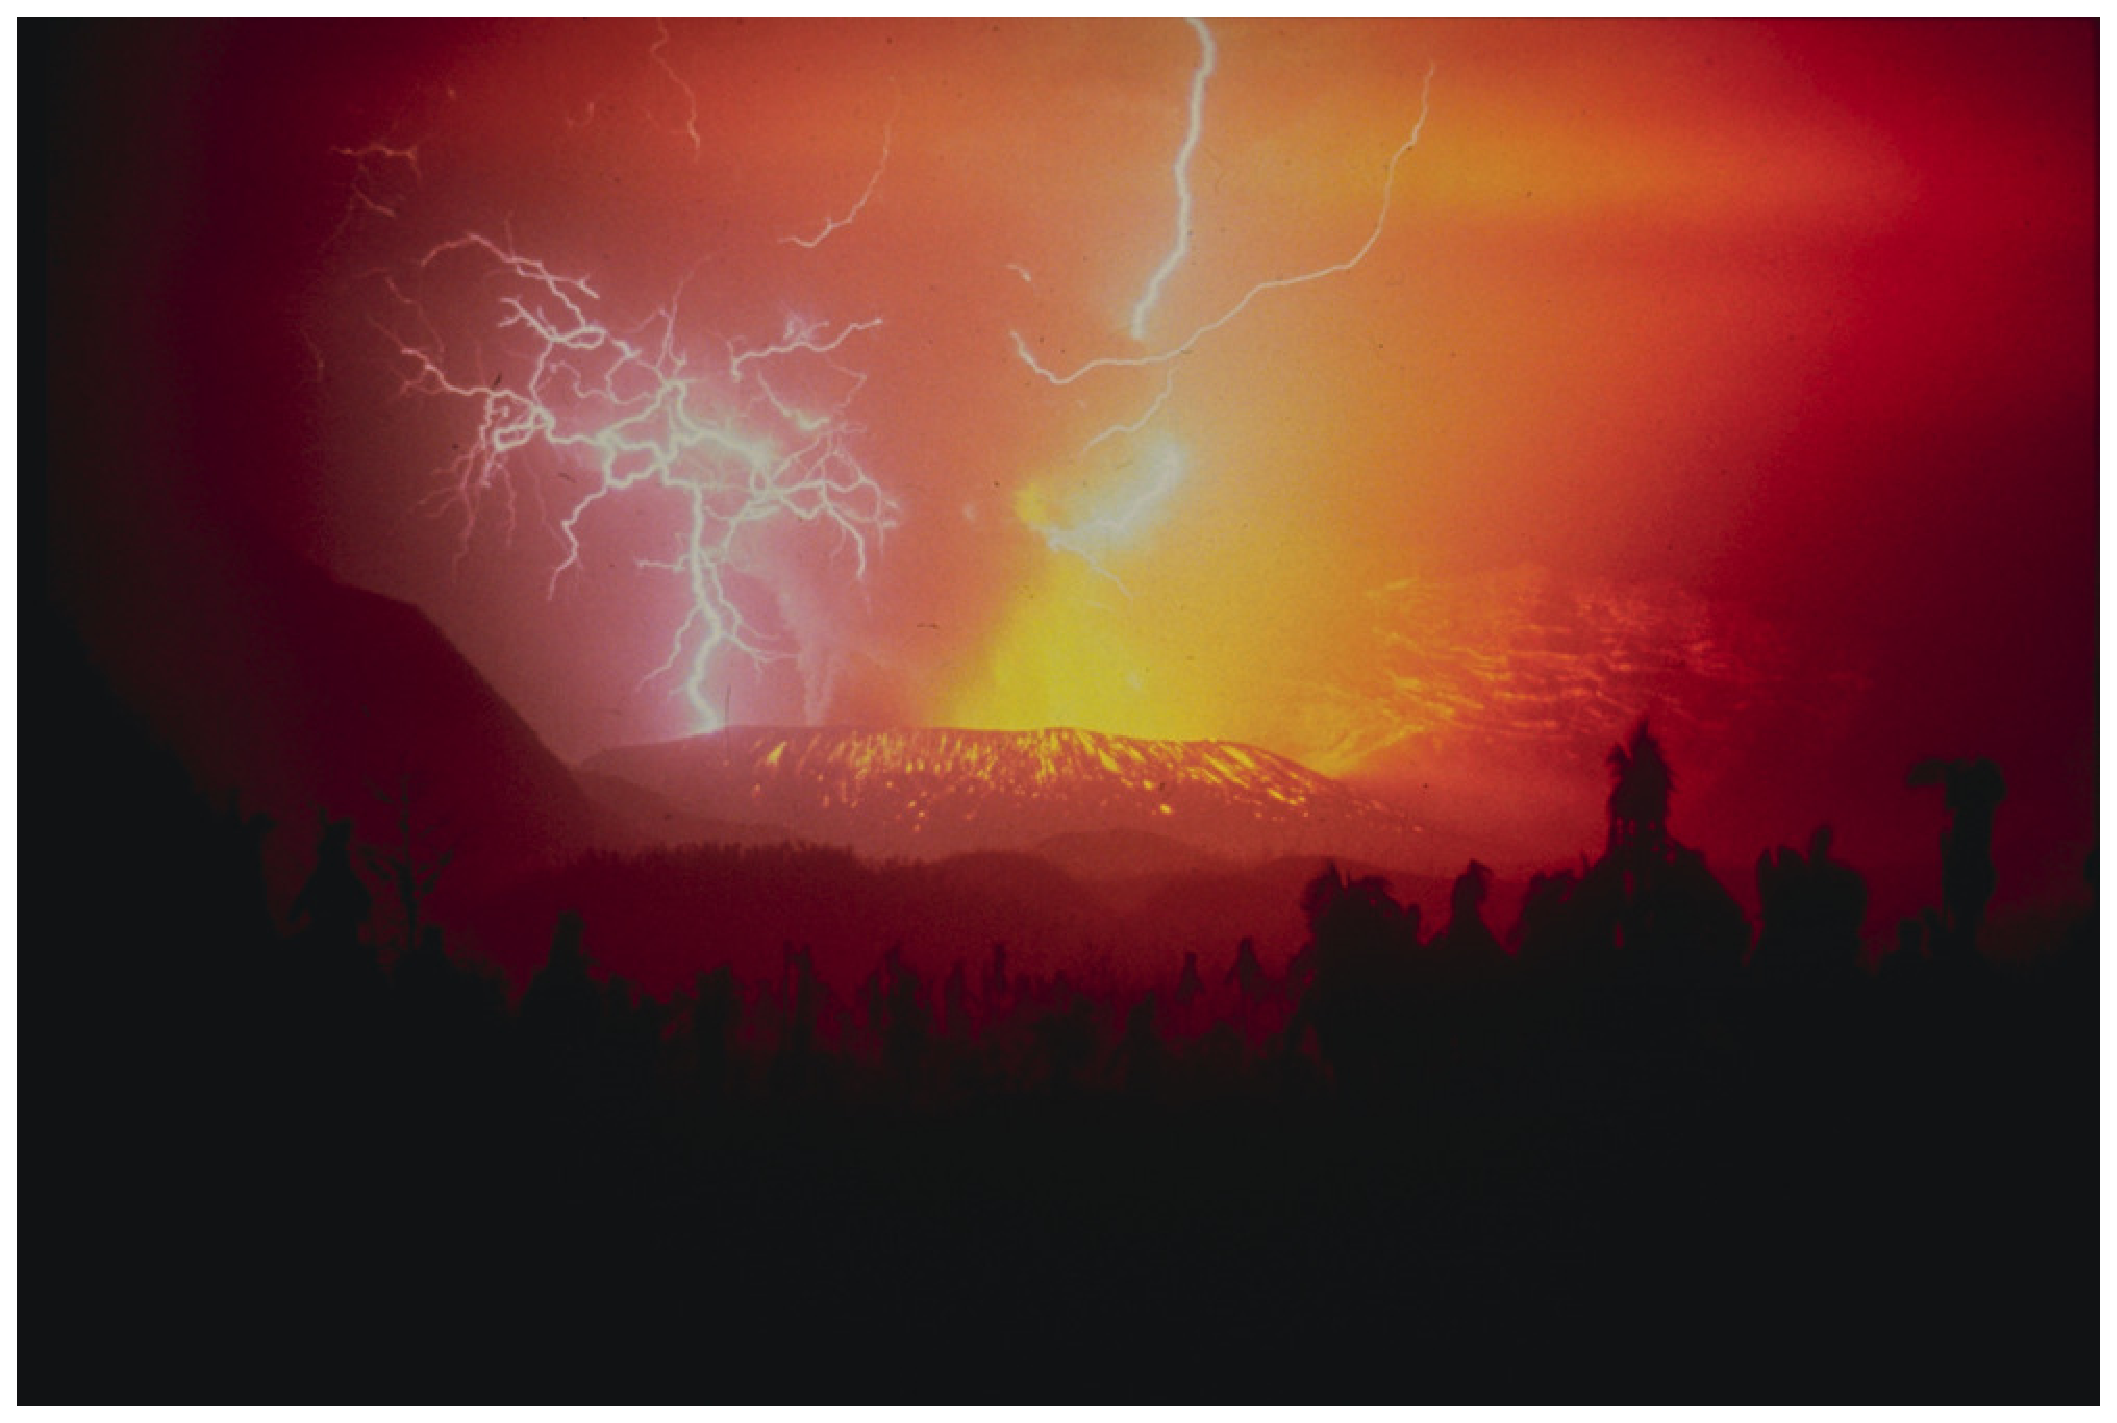
\includegraphics[width=0.6\textwidth]{foto2}%% Dimensões e localização
\fonte{\citet{Hadian1982}}%% Fonte
\end{photograph}

%% Título e rótulo de seção (rótulos não devem conter caracteres especiais, acentuados ou cedilha)
\subsection{Gráficos}\label{sec:graficos}

Gráficos são gerados com aplicativos capazes de exportar nos formatos \gls{ps} ou \gls{eps}. A ferramenta ``gnuplot'' é uma das mais utilizadas para a geração de gráficos (\url{http://www.gnuplot.info/}). Uma vez no formato \gls{eps}, gráficos são inseridos no texto tal como figuras, como pode ser observado no \autoref{gra:grafico1}.

\begin{graph}[htb]%% Ambiente graph
%\captionsetup{width=0.6\textwidth}%% Largura da legenda
\caption{Exemplo de gráfico produzido em ``gnuplot''}%% Legenda
\label{gra:grafico1}%% Rótulo
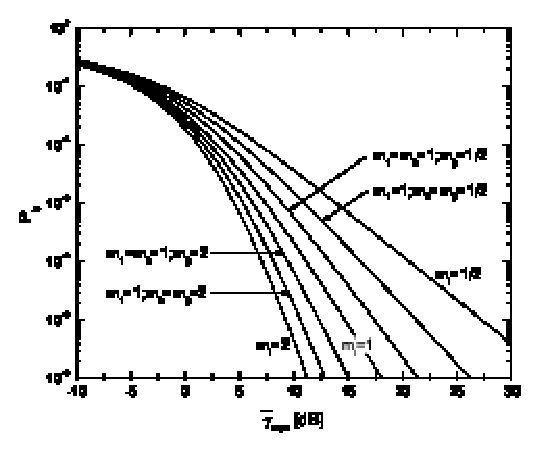
\includegraphics[width=0.6\textwidth]{grafico1}%% Dimensões e localização
\fonte{\citet{Faina2001}}%% Fonte
\end{graph}

No \autoref{gra:grafico2} é apresentado um exemplo de gráfico produzido em ``Excel''.

\begin{graph}[htb]%% Ambiente graph
%\captionsetup{width=0.6\textwidth}%% Largura da legenda
\caption{Exemplo de gráfico produzido em ``Excel''}%% Legenda
\label{gra:grafico2}%% Rótulo
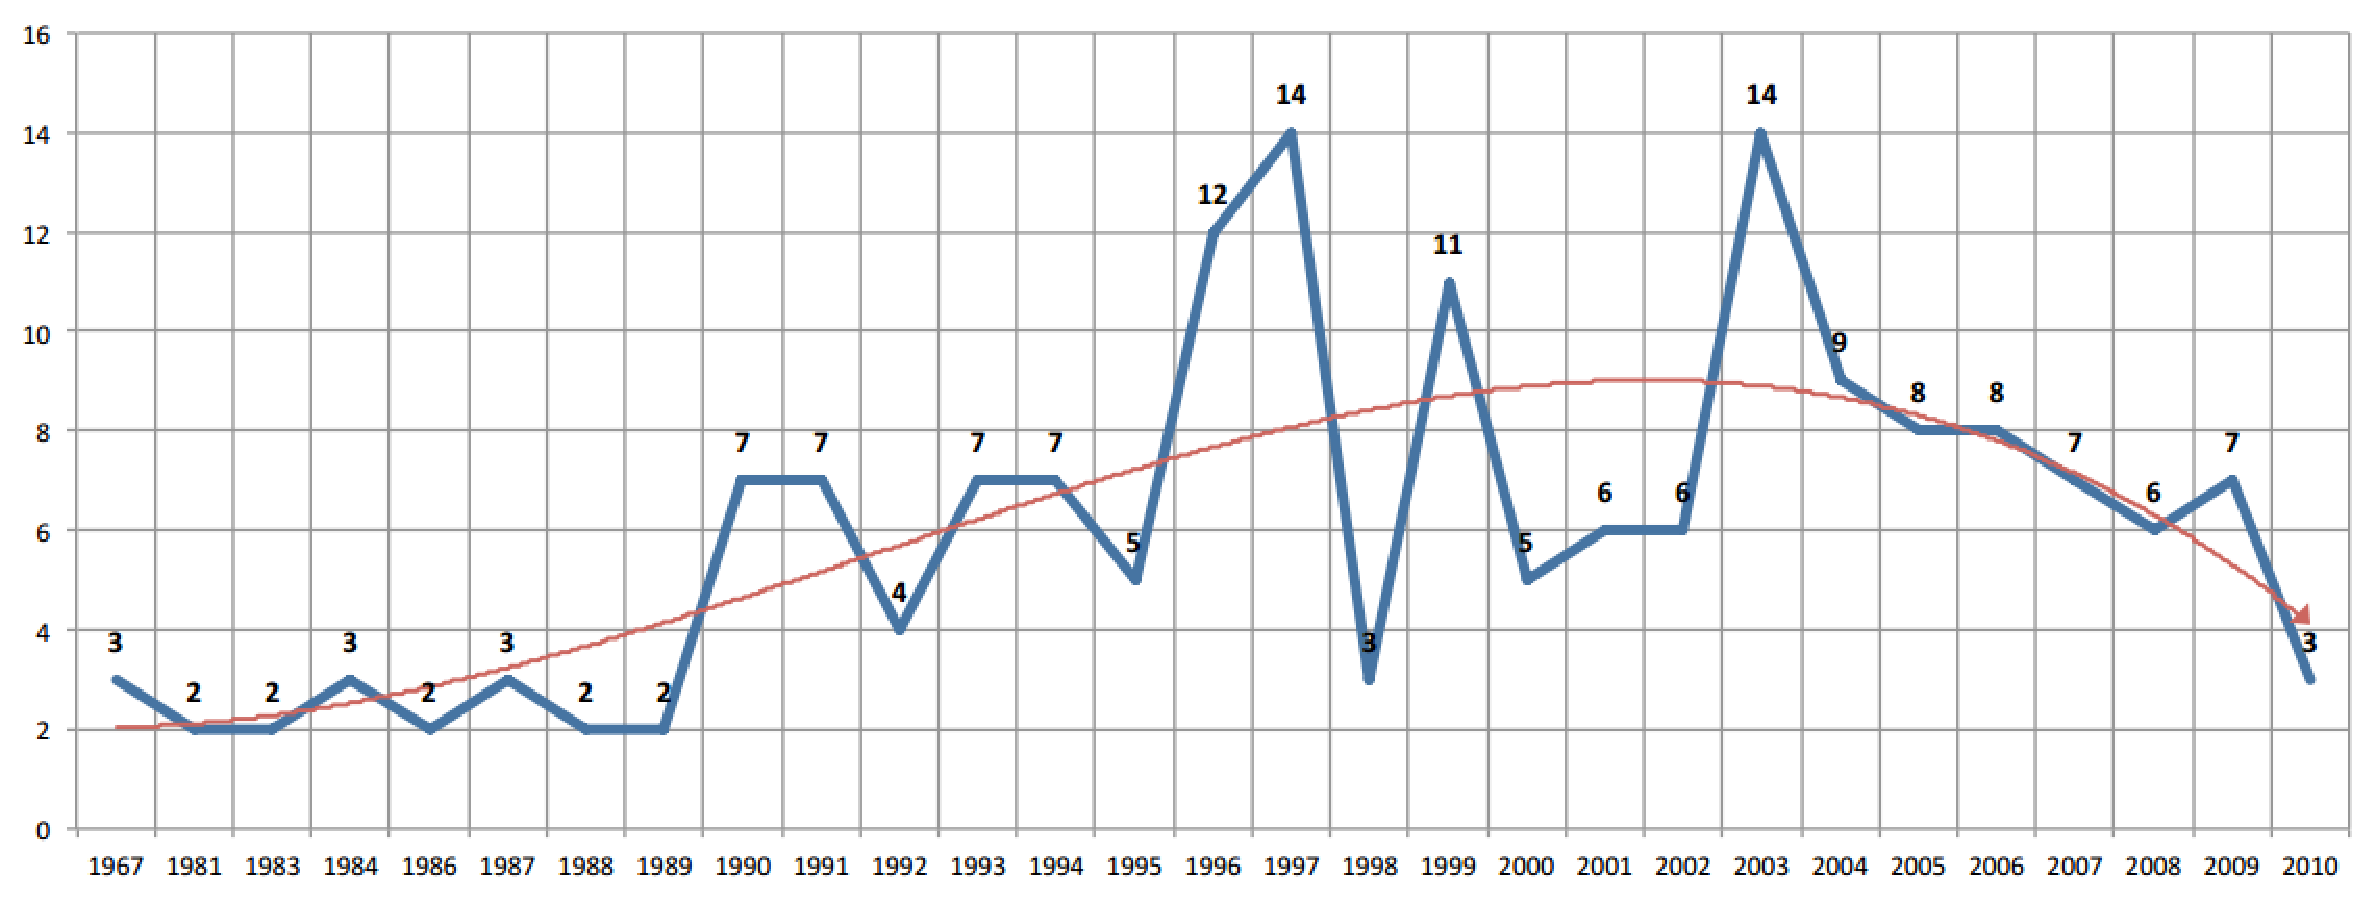
\includegraphics[width=0.6\textwidth]{grafico2}%% Dimensões e localização
\fonte{\citeonline[p. 24]{Araujo2012}}%% Fonte
\end{graph}

O ambiente \texttt{minipage} pode ser usado para inserir textos ou outros elementos em quadros com tamanhos e posições controladas, conforme exemplos apresentados no \autoref{gra:minipagegrafico1} e no \autoref{gra:minipagegrafico2}.

\begin{graph}[htb]%% Ambiente graph
\begin{minipage}[t]{0.395\textwidth}%% Ambiente minipage
\centering%% Centralizado
%\captionsetup{width=0.85\textwidth}%% Largura da legenda
\caption{Gráfico 1 do ambiente \texttt{minipage}}%% Legenda
\label{gra:minipagegrafico1}%% Rótulo
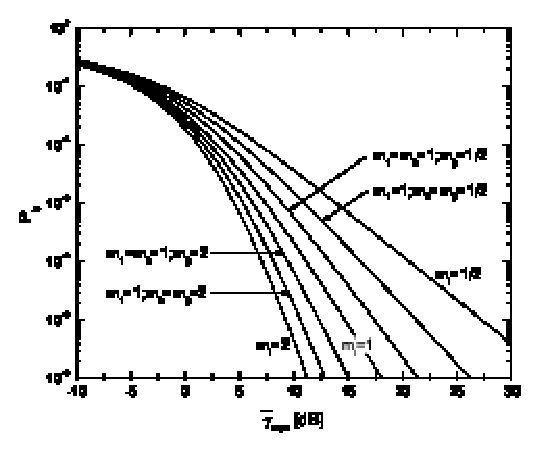
\includegraphics[width=0.85\textwidth]{grafico1}%% Dimensões e localização
\fonte{\citet{Faina2001}}%% Fonte
\end{minipage}
\hfill
\begin{minipage}[t]{0.595\textwidth}%% Ambiente minipage
\centering%% Centralizado
\captionsetup{width=0.95\textwidth}%% Largura da legenda
\caption{Gráfico 2 do ambiente \texttt{minipage}}%% Legenda
\label{gra:minipagegrafico2}%% Rótulo
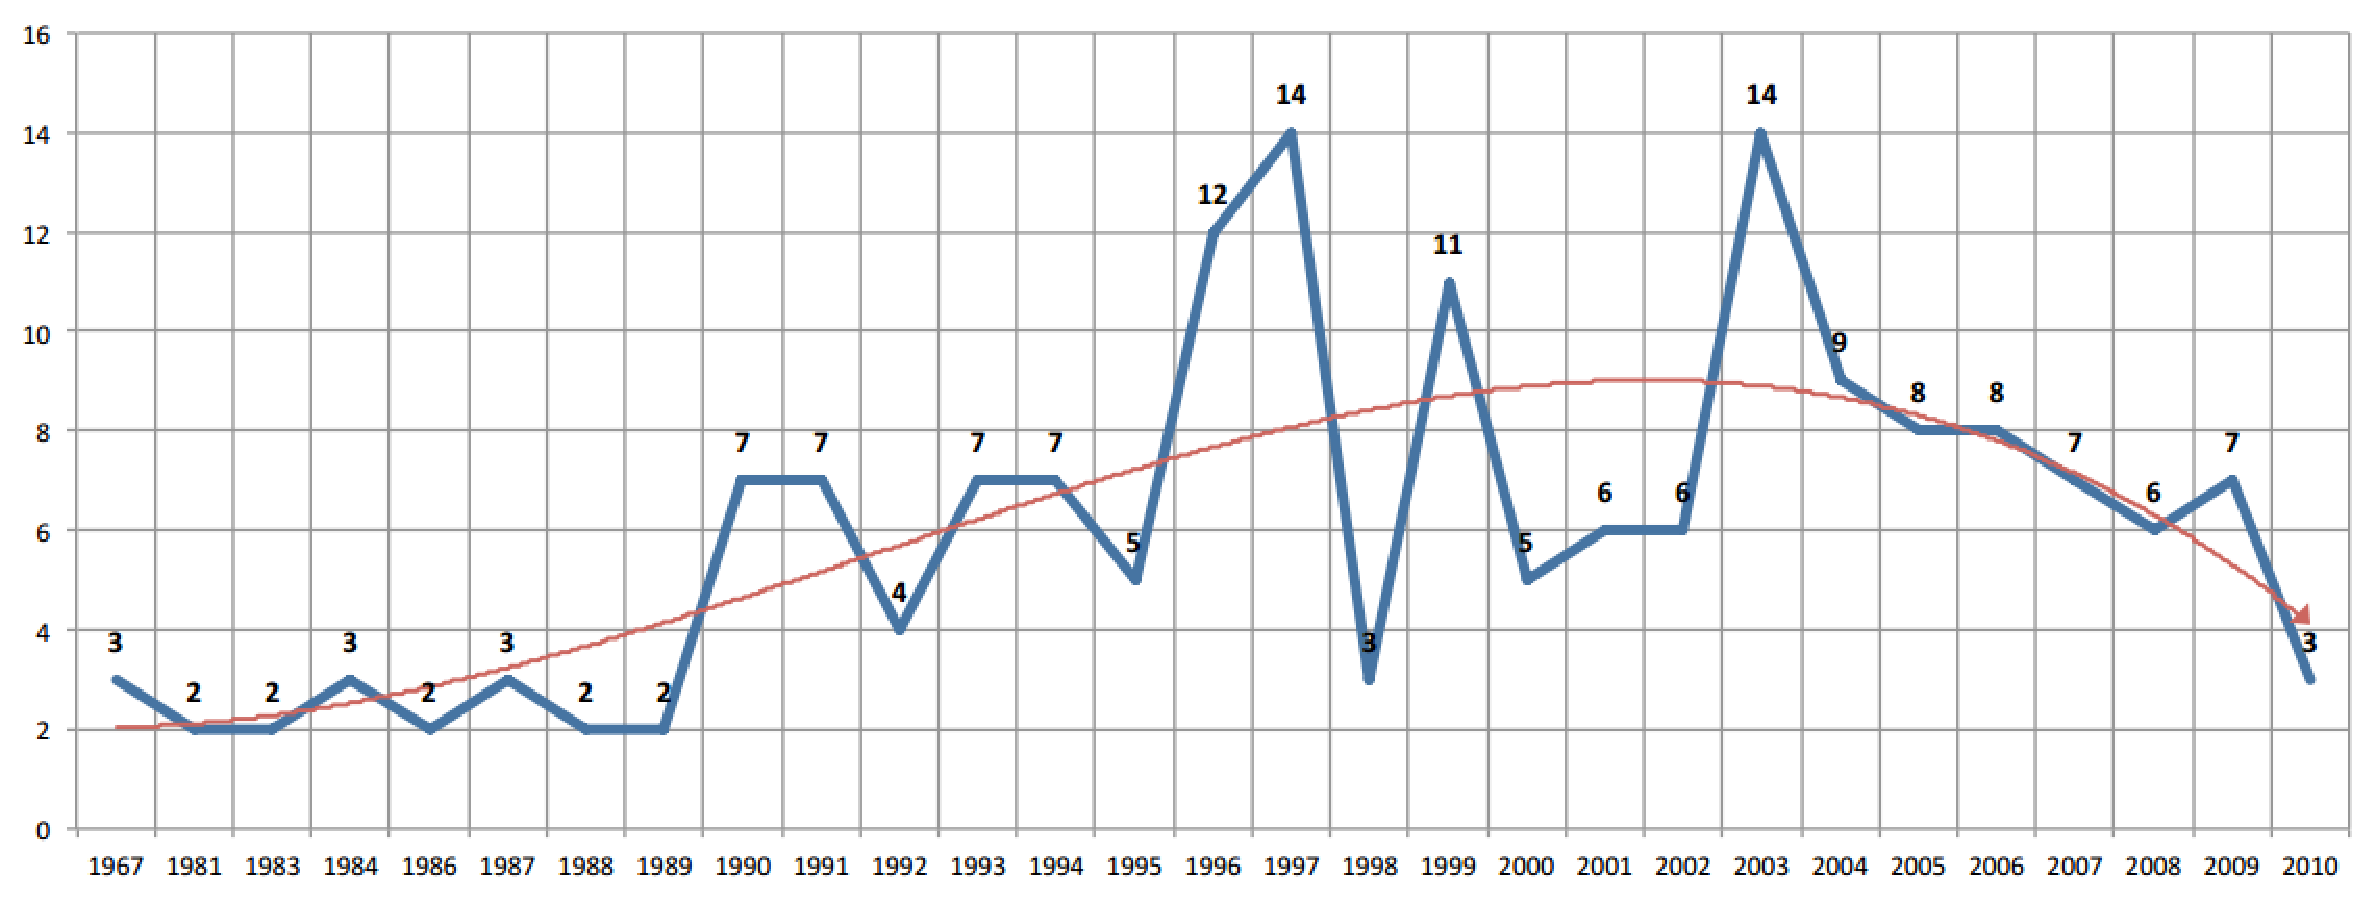
\includegraphics[width=0.95\textwidth]{grafico2}%% Dimensões e localização
\fonte{\citeonline[p. 24]{Araujo2012}}%% Fonte
\end{minipage}
\label{gra:minipagegraficos}
\end{graph}

%% Título e rótulo de seção (rótulos não devem conter caracteres especiais, acentuados ou cedilha)
\subsection{Quadros}\label{sec:quadros}

Um exemplo deste tipo de ilustração é apresentado no \autoref{quad:quadro1}.

\begin{tabframed}[htb]%% Ambiente tabframed
%\captionsetup{width=0.5\textwidth}%% Largura da legenda
\caption{Compostos orgânicos: fórmulas estruturais e principais classes}%% Legenda
\label{quad:quadro1}%% Rótulo
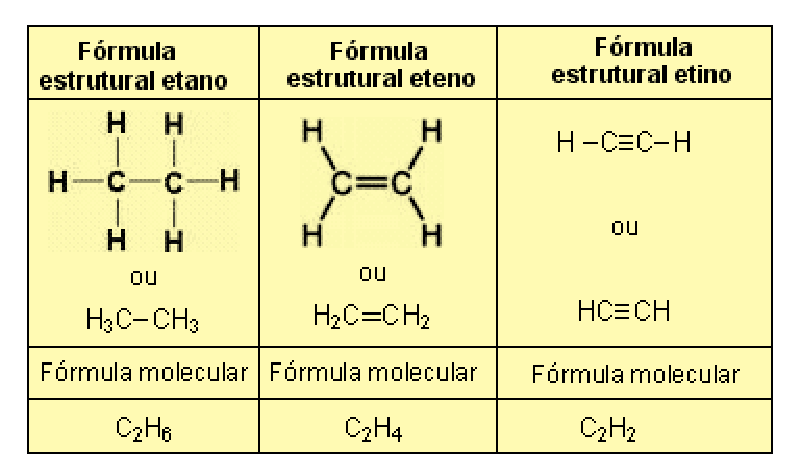
\includegraphics[width=0.5\textwidth]{quadro1}%% Dimensões e localização
\fonte{\citet{daSilva2009}}%% Fonte
\end{tabframed}

Outro exemplo deste tipo de ilustração é apresentado no \autoref{quad:quadro2}.

\begin{tabframed}[htb]%% Ambiente tabframed
%\captionsetup{width=0.7\textwidth}%% Largura da legenda
\caption{Modelos de maturidade para a gestão da cadeia de suprimentos}%% Legenda
\label{quad:quadro2}%% Rótulo
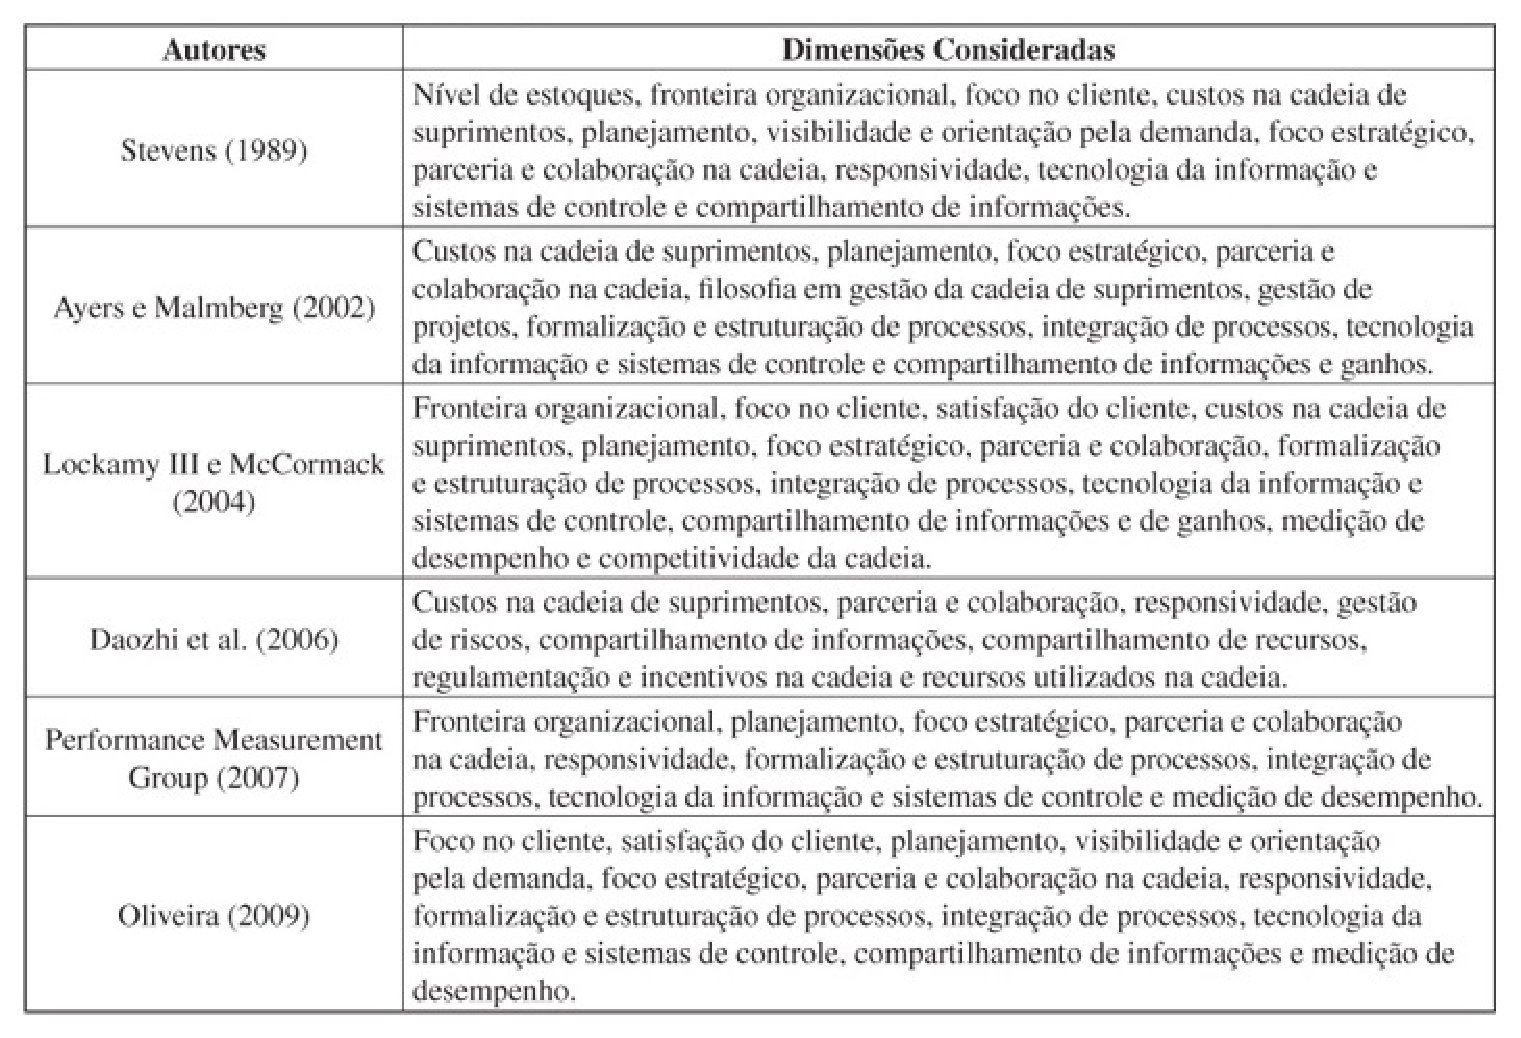
\includegraphics[width=0.7\textwidth]{quadro2}%% Dimensões e localização
\fonte{\citet{Frederico2012}}%% Fonte
\end{tabframed}

Os quadros não devem ser chamados de tabelas, uma vez que se diferenciam destas por apresentarem as laterais fechadas e o conteúdo não numérico.

%% Título e rótulo de seção (rótulos não devem conter caracteres especiais, acentuados ou cedilha)
\section{Tabelas}\label{sec:tabelas}

Tabelas são construídas com comandos próprios do \gls{latex}\index{LaTeX@\latex}. Por exemplo, a \autoref{tab:tabela1} foi construída desta forma.

\begin{table}[htb]%% Ambiente table
\caption{Primeiro exemplo de tabela com uma legenda contendo um texto muito longo que pode ocupar mais de uma linha}%% Legenda
\label{tab:tabela1}%% Rótulo
\begin{tabularx}{\textwidth}{@{\extracolsep{\fill}}llll}%% Ambiente tabularx
\toprule
$\bsym{L}$ & $\bsym{L^2}$ & $\bsym{L^3}$ & $\bsym{L^4}$ \\
\SI{}{[m]} & \SI{}{[m^2]} & \SI{}{[m^3]} & \SI{}{[m^4]} \\ \midrule
1          & 1            & 1            & 1            \\
2          & 4            & 8            & 16           \\
3          & 9            & 27           & 81           \\
4          & 16           & 64           & 256          \\
5          & 25           & 125          & 625          \\ \bottomrule
\end{tabularx}
\fonte{}%% Fonte
\end{table}

A \autoref{tab:tabela2} é um exemplo de tabela que ocupa mais de uma página e que foi construída pelo \gls{latex}\index{LaTeX@\latex} utilizando o pacote \texttt{longtable}.

\begin{longtable}{@{\extracolsep{\fill}}lll}%% Ambiente longtable
\caption{Possíveis tríplices para grade altamente variável\label{tab:tabela2}} \\%% Legenda e rótulo
\toprule
\textbf{Tempo (s)} & \textbf{Tríplice escolhida} & \textbf{Outras possíveis tríplices} \\
\midrule
\endfirsthead%% Encerra cabeçalho da primeira página
\caption[]{Possíveis tríplices para grade altamente variável} \\%% Legenda
\multicolumn{3}{r}{\textbf{(continuação)}} \\
\toprule
\textbf{Tempo (s)} & \textbf{Tríplice escolhida} & \textbf{Outras possíveis tríplices} \\
\midrule
\endhead%% Encerra cabeçalho das demais páginas
\midrule
\multicolumn{3}{r}{\textbf{(continua)}} \\
\endfoot%% Encerra rodapé das demais páginas
\bottomrule
\\[-0.5\linha]
\caption*{\nomefonte: Adaptado de \citet{Smallen2014}.} \\
\endlastfoot%% Encerra rodapé da última página
0      & (1, 11, 13725) & (1, 12, 10980), (1, 13, 8235), (2, 2, 0), (3, 1, 0) \\
2745   & (1, 12, 10980) & (1, 13, 8235), (2, 2, 0), (2, 3, 0), (3, 1, 0)      \\
5490   & (1, 12, 13725) & (2, 2, 2745), (2, 3, 0), (3, 1, 0)                  \\
8235   & (1, 12, 16470) & (1, 13, 13725), (2, 2, 2745), (2, 3, 0), (3, 1, 0)  \\
10980  & (1, 12, 16470) & (1, 13, 13725), (2, 2, 2745), (2, 3, 0), (3, 1, 0)  \\
13725  & (1, 12, 16470) & (1, 13, 13725), (2, 2, 2745), (2, 3, 0), (3, 1, 0)  \\
16470  & (1, 13, 16470) & (2, 2, 2745), (2, 3, 0), (3, 1, 0)                  \\
19215  & (1, 12, 16470) & (1, 13, 13725), (2, 2, 2745), (2, 3, 0), (3, 1, 0)  \\
21960  & (1, 12, 16470) & (1, 13, 13725), (2, 2, 2745), (2, 3, 0), (3, 1, 0)  \\
24705  & (1, 12, 16470) & (1, 13, 13725), (2, 2, 2745), (2, 3, 0), (3, 1, 0)  \\
27450  & (1, 12, 16470) & (1, 13, 13725), (2, 2, 2745), (2, 3, 0), (3, 1, 0)  \\
30195  & (2, 2, 2745)   & (2, 3, 0), (3, 1, 0)                                \\
32940  & (1, 13, 16470) & (2, 2, 2745), (2, 3, 0), (3, 1, 0)                  \\
35685  & (1, 13, 13725) & (2, 2, 2745), (2, 3, 0), (3, 1, 0)                  \\
38430  & (1, 13, 10980) & (2, 2, 2745), (2, 3, 0), (3, 1, 0)                  \\
41175  & (1, 12, 13725) & (1, 13, 10980), (2, 2, 2745), (2, 3, 0), (3, 1, 0)  \\
43920  & (1, 13, 10980) & (2, 2, 2745), (2, 3, 0), (3, 1, 0)                  \\
46665  & (2, 2, 2745)   & (2, 3, 0), (3, 1, 0)                                \\
49410  & (2, 2, 2745)   & (2, 3, 0), (3, 1, 0)                                \\
52155  & (1, 12, 16470) & (1, 13, 13725), (2, 2, 2745), (2, 3, 0), (3, 1, 0)  \\
54900  & (1, 13, 13725) & (2, 2, 2745), (2, 3, 0), (3, 1, 0)                  \\
57645  & (1, 13, 13725) & (2, 2, 2745), (2, 3, 0), (3, 1, 0)                  \\
60390  & (1, 12, 13725) & (2, 2, 2745), (2, 3, 0), (3, 1, 0)                  \\
63135  & (1, 13, 16470) & (2, 2, 2745), (2, 3, 0), (3, 1, 0)                  \\
65880  & (1, 13, 16470) & (2, 2, 2745), (2, 3, 0), (3, 1, 0)                  \\
68625  & (2, 2, 2745)   & (2, 3, 0), (3, 1, 0)                                \\
71370  & (1, 13, 13725) & (2, 2, 2745), (2, 3, 0), (3, 1, 0)                  \\
74115  & (1, 12, 13725) & (2, 2, 2745), (2, 3, 0), (3, 1, 0)                  \\
76860  & (1, 13, 13725) & (2, 2, 2745), (2, 3, 0), (3, 1, 0)                  \\
79605  & (1, 13, 13725) & (2, 2, 2745), (2, 3, 0), (3, 1, 0)                  \\
82350  & (1, 12, 13725) & (2, 2, 2745), (2, 3, 0), (3, 1, 0)                  \\
85095  & (1, 12, 13725) & (1, 13, 10980), (2, 2, 2745), (2, 3, 0), (3, 1, 0)  \\
87840  & (1, 13, 16470) & (2, 2, 2745), (2, 3, 0), (3, 1, 0)                  \\
90585  & (1, 13, 16470) & (2, 2, 2745), (2, 3, 0), (3, 1, 0)                  \\
93330  & (1, 13, 13725) & (2, 2, 2745), (2, 3, 0), (3, 1, 0)                  \\
96075  & (1, 13, 16470) & (2, 2, 2745), (2, 3, 0), (3, 1, 0)                  \\
98820  & (1, 13, 16470) & (2, 2, 2745), (2, 3, 0), (3, 1, 0)                  \\
101565 & (1, 13, 13725) & (2, 2, 2745), (2, 3, 0), (3, 1, 0)                  \\
104310 & (1, 13, 16470) & (2, 2, 2745), (2, 3, 0), (3, 1, 0)                  \\
107055 & (1, 13, 13725) & (2, 2, 2745), (2, 3, 0), (3, 1, 0)                  \\
109800 & (1, 13, 13725) & (2, 2, 2745), (2, 3, 0), (3, 1, 0)                  \\
112545 & (1, 12, 16470) & (1, 13, 13725), (2, 2, 2745), (2, 3, 0), (3, 1, 0)  \\
115290 & (1, 13, 16470) & (2, 2, 2745), (2, 3, 0), (3, 1, 0)                  \\
118035 & (1, 13, 13725) & (2, 2, 2745), (2, 3, 0), (3, 1, 0)                  \\
120780 & (1, 13, 16470) & (2, 2, 2745), (2, 3, 0), (3, 1, 0)                  \\
123525 & (1, 13, 13725) & (2, 2, 2745), (2, 3, 0), (3, 1, 0)                  \\
126270 & (1, 12, 16470) & (1, 13, 13725), (2, 2, 2745), (2, 3, 0), (3, 1, 0)  \\
129015 & (2, 2, 2745)   & (2, 3, 0), (3, 1, 0)                                \\
131760 & (2, 2, 2745)   & (2, 3, 0), (3, 1, 0)                                \\
134505 & (1, 13, 16470) & (2, 2, 2745), (2, 3, 0), (3, 1, 0)                  \\
137250 & (1, 13, 13725) & (2, 2, 2745), (2, 3, 0), (3, 1, 0)                  \\
139995 & (2, 2, 2745)   & (2, 3, 0), (3, 1, 0)                                \\
142740 & (2, 2, 2745)   & (2, 3, 0), (3, 1, 0)                                \\
145485 & (1, 12, 16470) & (1, 13, 13725), (2, 2, 2745), (2, 3, 0), (3, 1, 0)  \\
148230 & (2, 2, 2745)   & (2, 3, 0), (3, 1, 0)                                \\
150975 & (1, 13, 16470) & (2, 2, 2745), (2, 3, 0), (3, 1, 0)                  \\
153720 & (1, 12, 13725) & (2, 2, 2745), (2, 3, 0), (3, 1, 0)                  \\
156465 & (1, 13, 13725) & (2, 2, 2745), (2, 3, 0), (3, 1, 0)                  \\
159210 & (1, 13, 13725) & (2, 2, 2745), (2, 3, 0), (3, 1, 0)                  \\
161955 & (1, 13, 16470) & (2, 2, 2745), (2, 3, 0), (3, 1, 0)                  \\
164700 & (1, 13, 13725) & (2, 2, 2745), (2, 3, 0), (3, 1, 0)                  \\
\end{longtable}

Tabelas criadas em planilhas do ``Excel'' podem ser convertidas em tabelas \gls{latex}\index{LaTeX@\latex} utilizando o suplemento ``Excel-to-LaTeX'', disponível em \url{http://www.ctan.org/pkg/excel2latex}.

\textbf{Atenção!} É fortemente recomendável que as tabelas sejam criadas através de ferramentas \textit{online} ou \textit{plugins} do LibreOffice ou Microsoft Office, pois assim o trabalho de criar as tabelas fica bem mais fácil. Seguem \textit{links} de sítios \textit{online} que permitem criar tais tabelas, depois só é necessário copiar o código da tabela gerada por esses sítios para o texto do trabalho em \gls{latex}\index{LaTeX@\latex}:
\begin{itemize}
    \item \url{https://www.tablesgenerator.com/};
    \item \url{https://www.latex-tables.com/};
    \item \url{https://tableconvert.com/latex-generator};
    \item É possível buscar por outras na Internet através de termos de busca como ``latex table online'' ou ``latex criar tabela online''.
\end{itemize}

%% Título e rótulo de seção (rótulos não devem conter caracteres especiais, acentuados ou cedilha)
\section{Abreviaturas e siglas}\label{sec:acronimos}

\gls{latex}\index{LaTeX@\latex} gera automaticamente a lista de abreviaturas e siglaspor meio do pacote \texttt{glossaries}. As abreviaturas e siglas devem ser definidos no arquivo \texttt{entradas-acronimos.tex}, no diretório ``PreTexto'', com os comandos:

\begin{SingleSpacing}%% Ambiente SingleSpacing
\begin{verbatim}
\abreviatura{rótulo}{representação}{definição}
\sigla{rótulo}{representação}{definição}
\acronimo{rótulo}{representação}{definição}
\end{verbatim}
\end{SingleSpacing}

Para que a abreviatura ou sigla seja apresentada em alguma parte do texto do documento use o comando \verb|\gls{rótulo}|, por exemplo, as abreviaturas \gls{art.}, \gls{cap.} e \gls{sec.} foram geradas pelos comandos \verb|\gls{art.}, \gls{cap.} e \gls{sec.}|, respectivamente. Mais detalhes dos comandos do pacote \texttt{glossaries} podem ser encontrados em: \url{http://mirrors.ctan.org/macros/latex/contrib/glossaries/glossaries-user.pdf}.

Outra opção para gerar a lista de abreviaturas e siglas é por meio da edição manual do arquivo \texttt{lista-acronimos.tex} no diretório ``PreTexto''.

%% Título e rótulo de seção (rótulos não devem conter caracteres especiais, acentuados ou cedilha)
\section{Símbolos}\label{sec:simbolos}

\gls{latex}\index{LaTeX@\latex} gera automaticamente a lista de símbolos por meio do pacote \texttt{nomencl}. Ao redigir um símbolo pela primeira vez em qualquer parte do texto com o comando \verb|\nomenclature[prefixo]{símbolo}{descrição \nomunit{unidade}}|, é gerada uma entrada para a lista de símbolos. Veja exemplos deste comando no arquivo fonte deste capítulo. Os elementos da lista de símbolos são agrupados a depender da primeira letra atribuída ao prefixo e classificadas em:

\begin{itemize}%% Lista de itens
\item Letras Latinas.
\item Letras Gregas.
\item Sobrescritos.
\item Subscritos.
\item Notações.
\end{itemize}

Outra opção ao comando \verb|\nomenclature| é o uso dos atalhos:

\begin{SingleSpacing}%% Ambiente SingleSpacing
\begin{verbatim}
\letralatina{prefixo}{símbolo}{descrição}{unidade}
\letragrega{prefixo}{símbolo}{descrição}{unidade}
\sobrescrito{prefixo}{símbolo}{descrição}{unidade}
\subscrito{prefixo}{símbolo}{descrição}{unidade}
\notacao{prefixo}{símbolo}{descrição}{unidade}
\end{verbatim}
\end{SingleSpacing}

\noindent Neste caso a atribuição da primeira letra do prefixo pode ser desprezada.

%% Letras Latinas [A]
\nomenclature[AA]{$A$}{Área \nomunit{m^2}}%%
\letralatina{L}{L}{Comprimento}{m}%%
\letralatina{R}{R}{Raio}{m}%%
%% Letras Gregas [B]
\nomenclature[Bmu]{$\mu$}{Viscosidade dinâmica \nomunit{kg/(m.s)}}%%
\letragrega{nu}{\nu}{Viscosidade cinemática}{m^2/s}%%
\letragrega{pi}{\pi}{Pi (constante circular)}{rad}%%
\letragrega{rho}{\rho}{Massa específica}{kg/m^3}%%
\letragrega{sigma}{\sigma}{Tensão superficial}{N/m}%%
%% Sobrescritos [C]
\nomenclature[C+]{$+$}{Passo de tempo posterior}%%
\sobrescrito{-}{-}{Passo de tempo anterior}{}%%
\sobrescrito{0}{0}{Valor inicial}{}%%
%% Subscritos [D]
\nomenclature[DG]{$G$}{Fase gasosa}%%
\subscrito{L}{L}{Fase líquida}{}%%
\subscrito{S}{S}{Fase sólida}{}%%
%% Notações [E]
\nomenclature[EPsi_1]{$\overline{\Psi}$}{Média temporal}%%
\notacao{Psi_2}{\langle \Psi \rangle}{Média na seção transversal}{}%%
\notacao{Psi_3}{\langle\langle \Psi \rangle\rangle}{Média na seção transversal ponderada}{}%%

Mais detalhes dos comandos do pacote \texttt{nomencl} podem ser encontrados em: \url{http://tug.ctan.org/tex-archive/macros/latex/contrib/nomencl/nomencl.pdf}.

Outra opção para gerar a lista de símbolos é por meio da edição manual do arquivo \texttt{lista-simbolos.tex} no diretório ``PreTexto''.

%% Título e rótulo de seção (rótulos não devem conter caracteres especiais, acentuados ou cedilha)
\section{Inclusão de outros arquivos}\label{sec:inclusao}

É uma boa prática dividir o seu documento em diversos arquivos, e não apenas escrever tudo em um único. Esse recurso foi utilizado neste documento (veja \texttt{utfprpb.tex}). Para incluir diferentes arquivos em um arquivo principal, de modo que cada arquivo incluído fique em uma página diferente, utilize o comando:

\begin{SingleSpacing}%% Ambiente SingleSpacing
\begin{verbatim}
\include{documento-a-ser-incluido} %% Sem a extensão .tex
\end{verbatim}
\end{SingleSpacing}

Para incluir documentos sem quebra de páginas, utilize:

\begin{SingleSpacing}%% Ambiente SingleSpacing
\begin{verbatim}
\input{documento-a-ser-incluido}   %% Sem a extensão .tex
\end{verbatim}
\end{SingleSpacing}

%% Título e rótulo de seção (rótulos não devem conter caracteres especiais, acentuados ou cedilha)
\section{Referências}\label{sec:referencias}

A formatação das referências bibliográficas conforme as regras da \gls{abnt}\index{ABNT} são um dos principais objetivos do \gls{abntex2}\index{abnTeX2@\abnTeX}. Consulte os manuais \citeonline{abnTeX2:2013Cite} e \citeonline{abnTeX2:2013CiteAlf} para obter informações sobre sua utilização.

%% Título e rótulo de seção (rótulos não devem conter caracteres especiais, acentuados ou cedilha)
%\subsection{Acentuação de referências bibliográficas}\label{sec:acentuacaodereferencias}

Normalmente não há problemas em usar caracteres acentuados em arquivos bibliográficos (extensão \texttt{bib}). Porém, como as regras da \gls{abnt}\index{ABNT} fazem uso quase abusivo da conversão para letras maiúsculas, é preciso observar o modo como se escreve os nomes dos autores e/ou editores. No \autoref{quad:quadro3} você encontra alguns exemplos das conversões mais importantes. A regra geral é sempre usar a acentuação neste modo quando houver conversão para letras maiúsculas.

\begin{tabframed}[htb]%% Ambiente tabframed
%\captionsetup{width=0.5\textwidth}%% Largura da legenda
\caption{Conversão de acentuação em arquivos \texttt{bibtex}}%% Legenda
\label{quad:quadro3}%% Rótulo
\begin{tabular}{|*{2}{p{0.25\textwidth-\columnsep}|}}%% Ambiente tabular
\hline
\textbf{Acento}   & \textbf{Comando}                       \\ \hline
{\'a} {\`a} {\~a} & \verb|{\'a}| \verb|{\`a}| \verb|{\~a}| \\ \hline
{\^e}             & \verb|{\^e}|                           \\ \hline
{\"u}             & \verb|{\"u}|                           \\ \hline
{\'\i}            & \verb|{\'\i}|                          \\ \hline
{\c{c}}           & \verb|{\c{c}}|                         \\ \hline
\end{tabular}
\fonte{}%% Fonte
\end{tabframed}

%% Título e rótulo de seção (rótulos não devem conter caracteres especiais, acentuados ou cedilha)
\section{Glossário}\label{sec:glossario}

Você pode definir as entradas do glossário no início do texto. Recomenda-se o uso de um arquivo separado a ser inserido ainda no preâmbulo do documento, como por exemplo o arquivo \texttt{entradas-glossario.tex} no diretório ``PosTexto'' do presente documento. Veja orientações sobre inclusão de arquivos na \autoref{sec:inclusao}.

`O \gls{abntex2} é \glsdesc*{abntex2}' é um exemplo de termo definido no glossário e usado no decorrer do texto, bem como:

\begin{citacao}%% Ambiente citacao
Esta frase usa a palavra \gls{componente} e o plural de \glspl{filho}, ambas definidas no glossário como filhas da entrada \gls{pai}. \Gls{equilibrio} exemplifica o uso de um termo no início da frase. O software \gls{abntex2}\index{abnTeX2@\abnTeX} é escrito em \gls{latex}\index{LaTeX@\latex}, que é definido no glossário como `\glsdesc*{latex}'.
\end{citacao}

A frase da citação direta acima foi produzida com:

\begin{SingleSpacing}%% Ambiente SingleSpacing
\begin{verbatim}
Esta frase usa a palavra \gls{componente} e o plural de
\glspl{filho}, ambas definidas no glossário como filhas da
entrada \gls{pai}. \Gls{equilibrio} exemplifica o uso de um
termo no início da frase. O software \gls{abntex2} é
escrito em \gls{latex}, que é definido no glossário como
`\glsdesc*{latex}'.
\end{verbatim}
\end{SingleSpacing}

A impressão efetiva do glossário é dada com:

\begin{SingleSpacing}%% Ambiente SingleSpacing
\begin{verbatim}
\printglossaries
\end{verbatim}
\end{SingleSpacing}

A impressão do glossário incorpora o número das páginas em que as entradas foram citadas. Isso pode ser removido adicionando-se a opção \texttt{nonumberlist} em:

\begin{SingleSpacing}%% Ambiente SingleSpacing
\begin{verbatim}
\usepackage[nonumberlist, style=index]{glossaries}
\end{verbatim}
\end{SingleSpacing}

%% Título e rótulo de seção (rótulos não devem conter caracteres especiais, acentuados ou cedilha)
\section{Apêndices e anexos}\label{sec:apendiceseanexos}

Apêndices e anexos podem ser inseridos no documento, logo após o glossário, por meio da inclusão de arquivos, como por exemplo, os arquivos fontes \texttt{apendicea.tex}, \texttt{apendiceb.tex}, \texttt{anexoa.tex} e \texttt{anexob.tex}, presentes no diretório ``PosTexto'' deste projeto, são utilizados para gerar o \autoref{cap:apendicea}, o \autoref{cap:apendiceb}, o \autoref{cap:anexoa} e o \autoref{cap:anexob}, respectivamente. Veja orientações sobre inclusão de arquivos na \autoref{sec:inclusao}.

%% Título e rótulo de seção (rótulos não devem conter caracteres especiais, acentuados ou cedilha)
\section{Índice remissivo}\label{sec:indice}

Palavras podem ser indexadas no índice remissivo por meio do comando \verb|\index{palavra a ser indexada}|. Existem vários exemplos do uso deste comando no arquivo fonte deste capítulo. Por exemplo o comando \verb|\index{Windows}| é utilizado para indexar a palavra Windows\index{Windows} no índice remissivo.

%% Título e rótulo de seção (rótulos não devem conter caracteres especiais, acentuados ou cedilha)
\section{Compilação do documento latex}\label{sec:compilar}\index{LaTeX@\latex}

Geralmente os editores \gls{latex}\index{LaTeX@\latex}, como o TeXlipse\index{TeXlipse}\footnote{Disponível em \url{http://texlipse.sourceforge.net/}.}, o Texmaker\index{Texmaker}\footnote{Disponível em \url{http://www.xm1math.net/texmaker/}.}, entre outros, compilam os documentos automaticamente ou após configuração, de modo que você não precisa se preocupar com isto.

No entanto, você pode compilar os documentos \gls{latex}\index{LaTeX@\latex} usando os seguintes comandos, que devem ser digitados no \textit{Prompt} de comandos do Windows\index{Windows} ou no terminal do Mac\index{Mac} ou do Linux\index{Linux}:

\begin{SingleSpacing}%% Ambiente SingleSpacing
\begin{verbatim}
latex <mainfile>.tex
bibtex <mainfile>
latex <mainfile>.tex
latex <mainfile>.tex
dvips <dvips configs> <mainfile>.dvi -o <mainfile>.ps
ps2pdf <mainfile>.ps <mainfile>.pdf
\end{verbatim}
\end{SingleSpacing}

\noindent se todas as figuras no seu documento estão no formato \gls{eps}, ou então, usando os seguintes comandos:

\begin{SingleSpacing}%% Ambiente SingleSpacing
\begin{verbatim}
pdflatex <mainfile>.tex
bibtex <mainfile>
pdflatex <mainfile>.tex
pdflatex <mainfile>.tex
\end{verbatim}
\end{SingleSpacing}

\noindent se todas as figuras no seu documento estão no \gls{pdf}, ou em formatos comuns de imagens (BMP, GIF, JPG ou PNG).

%% Título e rótulo de seção (rótulos não devem conter caracteres especiais, acentuados ou cedilha)
\subsection{Problemas de compilação}\label{sec:problemas}

O \gls{utfprpbtex}\index{UTFPRPBTeX@\utfprtex} foi configurado e testado para compilar documentos \gls{latex}\index{LaTeX@\latex} sem problemas, mas por se tratar de uma linguagem de programação (para editoração) está sujeita a \textit{bugs} como qualquer outra linguagem. Além disto, o \gls{utfprpbtex}\index{UTFPRPBTeX@\utfprtex} é baseado em outras classes de documento e também utiliza uma quantidade considerável de pacotes que podem ter incompatibilidades. Portanto, alguns cuidados devem ser tomados quando se trabalha com \gls{latex}\index{LaTeX@\latex}, principalmente para novos usuários:

\begin{itemize}%% Lista de itens
\item Os comandos devem ser corretamente finalizados, ou seja, deve-se verificar a abertura e fechamento dos colchetes e chaves: \verb|\comando[opções]{argumentos}|. Alguns comandos não necessitam disto, por exemplo \verb|\comando|, mas as vezes torna-se necessário colocar uma barra invertida, \verb|\|, ou chaves, \verb|{}|, após o comando para gerar um espaço com o texto na sequência: \verb|\comando\ texto na sequência do comando| ou \verb|\comando{} texto na sequência do comando|.
\item Os ambientes devem ser corretamente finalizados, ou seja, deve-se verificar a abertura e fechamento dos ambientes: \verb|\begin{ambiente} ... \end{ambiente}|.
\item Os caracteres especiais devem ser precedidos de barra invertida quando se deseja imprimí-los no texto: \verb|\$ \& \% \# \_ \{ \}| resulta em \$ \& \% \# \_ \{ \}. Do contrário, não serão impressos e executarão comandos específicos do \gls{latex}\index{LaTeX@\latex}.
\item Os textos copiados de outros arquivos (\texttt{*.doc}, \texttt{*.html}, \texttt{*.pdf}, etc.) para os arquivos fonte do \gls{latex}\index{LaTeX@\latex} (\texttt{*.tex}, \texttt{*.bib}, etc.) devem ter a mesma codificação de caracteres (\texttt{UTF8}). Do contrário, alguns caracteres não serão devidamente impressos ou causarão erro, por exemplo, o hífen e os caracteres acentuados.
\item Os nomes de arquivos carregados no modelo (arquivos fontes, figuras, etc.) não devem conter caracteres especiais ou acentuados: \verb|capitulo1.tex| ao invés de \verb|capitulo_1.tex|. Esta regra também se aplica aos rótulos: \verb|\label{cap:capitulo1}| ao invés de \verb|\label{cap:capitulo_1}|.
\end{itemize}

Outras dicas de uso dos comandos do \gls{latex}\index{LaTeX@\latex} podem ser encontradas em diversos materiais de referência disponíveis na Internet, por exemplo: \url{http://en.wikibooks.org/wiki/LaTeX}, \url{http://repositorios.cpai.unb.br/ctan/info/lshort/portuguese-BR/lshortBR.pdf}, entre outros.

%% Licença utilizada no trabalho da UTFPR
\section{Licença}\label{sec:licenca}

De acordo com a Resolução Conjunta \href{https://sei.utfpr.edu.br/sei/publicacoes/controlador_publicacoes.php?acao=publicacao_visualizar&id_documento=1811618&id_orgao_publicacao=0}{nº 01/2020 COGEP-COPPG}, os trabalhos de conclusão de curso da \gls{utfpr} devem adotar uma licença Creative Commons, sendo que o texto das possíveis licenças pode ser visto em: \url{https://creativecommons.org/licenses/?lang=pt_BR}.

Para facilitar a adoção dessas licenças o presente \textit{template} possui o comando \texttt{$\backslash$licenca\{\}}, disponível no arquivo \texttt{variaveis.tex} do \textit{template}. As possibilidades para este comando são:

\begin{itemize}
    \item \texttt{$\backslash$licenca\{ccby\}} - para usar a licença CC BY (está como padrão no \textit{template}); 
    \item \texttt{$\backslash$licenca\{ccbysa\}} - para usar a licença CC BY CA;
    \item \texttt{$\backslash$licenca\{ccbynd\}} - para usar a licença CC BY ND;
    \item \texttt{$\backslash$licenca\{ccbync\}} - para usar a licença CC BY NC;
    \item \texttt{$\backslash$licenca\{ccbyncsa\}} - para usar a licença CC BY NC SA;
    \item \texttt{$\backslash$licenca\{ccbyncnd\}} - para usar a licença CC BY NC ND;
    \item \texttt{$\backslash$licenca\{\}} - deixar em branco, neste caso não aparecerá nenhuma licença (não recomendável).
\end{itemize}

Então, converse com o orientador a respeito de qual licença utilizar, localize o comando \texttt{$\backslash$licenca\{\}} no arquivo \texttt{variaveis.tex} e deixe descomentado (sem o \texttt{\%} no inicio da linha) apenas a licença que será utilizada no trabalho. Atenção, tome o cuidado de não deixar mais de uma licença desabilitada e confira se a licença escolhida é a que está aparecendo na Folha de Rosto do trabalho.%% Comente para remover este item

%% Parte
% \part{Conclusão}%% Comente para remover este item

%% Capítulo
% %%%% CAPÍTULO 5 - CONCLUSÕES E PERSPECTIVAS
%%
\chapter{Conclusão}\label{cap:conclusoeseperspectivas}

Inicia com um resumo do trabalho, retomando o(s) objetivo(s), o referencial teórico e o uso das ferramentas e das tecnologias utilizadas no trabalho.

A conclusão contém a opinião do autor em relação às vantagens, desvantagens, facilidades e limitações das tecnologias e/ou do método utilizados, as dificuldades encontradas e como foram superadas.

Também devem ser apresentadas as vantagens, desvantagens e limitações do trabalho desenvolvido, sempre tendo em vista a sua contribuição para a comunidade acadêmica e profissional e para a sociedade como um todo.

É a opinião técnica do autor do trabalho em relação ao assunto sob a forma de uma espécie de avaliação em relação ao trabalho desenvolvido e as tecnologias utilizadas.

Finaliza verificando se o objetivo foi alcançado e com a opinião do autor sobre o assunto, de acordo com o referencial teórico e com os resultados obtidos.

As perspectivas futuras são opcionais, devem ser apresentadas somente caso o acadêmico pretenda dar continuidade ao trabalho, ou mesmo se ele julgar relevante que outras pessoas dêem continuidade ao seu trabalho.
%% Comente para remover este item

%% Capítulo
\chapter{Cronograma}\label{cap:cronograma}

No \autoref{quad:cronograma} é apresentado o cronograma do trabalho. Proporcionando uma visão completa e organizada das atividades realizadas e planejadas ao longo do projeto.

\begin{tabframed}[htb]
  \caption{Cronograma}
  \label{quad:cronograma}
  \renewcommand{\arraystretch}{1.5}
  \begin{tabular}{|l|lllll|}
    \hline
    \multirow{2}{*}{Atividiades}                                &
    \multicolumn{5}{l|}{Meses}
    \\ \cline{2-6}

                                                                &
    \multicolumn{1}{l|}{Ago}                                    &
    \multicolumn{1}{l|}{Set}                                    &
    \multicolumn{1}{l|}{Out}                                    &
    \multicolumn{1}{l|}{Nov}                                    &
    \multicolumn{1}{l|}{Dez}
    \\ \hline

    Elaboração da proposta                                      &
    \multicolumn{1}{l|}{x}                                      &
    \multicolumn{1}{l|}{}                                       &
    \multicolumn{1}{l|}{}                                       &
    \multicolumn{1}{l|}{}                                       &
    \\ \hline

    Levantamento bibliográfico e escrita do referencial teórico &
    \multicolumn{1}{l|}{}                                       &
    \multicolumn{1}{l|}{x}                                      &
    \multicolumn{1}{l|}{}                                       &
    \multicolumn{1}{l|}{}                                       &
    \\ \hline

    Definição e documentação dos requisitos                     &
    \multicolumn{1}{l|}{}                                       &
    \multicolumn{1}{l|}{x}                                      &
    \multicolumn{1}{l|}{x}                                      &
    \multicolumn{1}{l|}{}                                       &
    \\ \hline

    Escrita TCC 1                                               &
    \multicolumn{1}{l|}{}                                       &
    \multicolumn{1}{l|}{x}                                      &
    \multicolumn{1}{l|}{x}                                      &
    \multicolumn{1}{l|}{x}                                      &
    \\ \hline

    Modelagem do sistema                                        &
    \multicolumn{1}{l|}{}                                       &
    \multicolumn{1}{l|}{}                                       &
    \multicolumn{1}{l|}{}                                       &
    \multicolumn{1}{l|}{x}                                      &
    \\ \hline

    Elaboração da apresentação do TCC 1                         &
    \multicolumn{1}{l|}{}                                       &
    \multicolumn{1}{l|}{}                                       &
    \multicolumn{1}{l|}{}                                       &
    \multicolumn{1}{l|}{x}                                      &
    \\ \hline

    Apresentação TCC 1                                          &
    \multicolumn{1}{l|}{}                                       &
    \multicolumn{1}{l|}{}                                       &
    \multicolumn{1}{l|}{}                                       &
    \multicolumn{1}{l|}{}                                       &
    \multicolumn{1}{l|}{x}
    \\ \hline
  \end{tabular}
  \fonte{} % Fonte
\end{tabframed}
%% Comente para remover este item

%% Capítulos após este comando criam marcadores do pdf na raiz
% \phantompart%% Comente para remover este item


%% Formatação de páginas de elementos pós-textuais
\postextual%% Não comente esta linha

%% Arquivos de referências
\arquivosdereferencias{%% Arquivos bibtex sem a extensão .bib e separados por vírgula - Não comente esta linha
  %./PosTexto/exemplos-referencias,%% Arquivo de referências - Comente para remover este item
  main%% Arquivo de referências - Comente para remover este item
}%% Não comente esta linha

%% Glossário
%\incluirglossario %% Comente para remover este item

%% Arquivos de apêndices
 \begin{arquivosdeapendices}%% Os arquivos de apêndices devem se incluídos neste ambiente - Não comente esta linha
%   %\partapendices%% Página de início dos apêndices - adiciona uma página com o título Apêndices
%   %% Capítulo de exemplo
  %  %%%% APÊNDICE A
%%
%% Texto ou documento elaborado pelo autor, a fim de complementar sua argumentação, sem prejuízo da unidade nuclear do trabalho.

%% Título e rótulo de apêndice (rótulos não devem conter caracteres especiais, acentuados ou cedilha)
\chapter{Título do Apêndice A com um Texto Muito Longo que Pode Ocupar Mais de uma Linha}\label{cap:apendicea}

Quando houver necessidade pode-se apresentar como apêndice documento(s) auxiliar(es) e/ou complementar(es) como: legislação, estatutos, gráficos, tabelas, etc. Os apêndices são enumerados com letras maiúsculas: \autoref{cap:apendicea}, \autoref{cap:apendiceb}, etc.

No \latex\ apêndices são editados como capítulos. O comando \verb|\appendix| faz com que todos os capítulos seguintes sejam considerados apêndices.

Apêndices complementam o texto principal da tese com informações para leitores com especial interesse no tema, devendo ser considerados leitura opcional, ou seja, o entendimento do texto principal da tese não deve exigir a leitura atenta dos apêndices.

Apêndices usualmente contemplam provas de teoremas, deduções de fórmulas matemáticas, diagramas esquemáticos, gráficos e trechos de código. Quanto a este último, código extenso não deve fazer parte da tese, mesmo como apêndice. O ideal é disponibilizar o código na Internet para os interessados em examiná-lo ou utilizá-lo.

%% Título e rótulo de seção (rótulos não devem conter caracteres especiais, acentuados ou cedilha)
%\section{Título da Seção Secundária do Apêndice B}\label{sec:secaoapendicea}

%Exemplo de seção secundária em apêndice (\autoref{sec:secaoapendicea} do \autoref{cap:apendicea}).

%% Título e rótulo de seção (rótulos não devem conter caracteres especiais, acentuados ou cedilha)
%\subsection{Título da Seção Terciária do Apêndice B}\label{subsec:subsecaoapendicea}

%Exemplo de seção terciária em apêndice (\autoref{subsec:subsecaoapendicea} do \autoref{cap:apendicea}).

%% Título e rótulo de seção (rótulos não devem conter caracteres especiais, acentuados ou cedilha)
%\subsubsection{Título da seção quaternária do Apêndice B}\label{subsubsec:subsubsecaoapendicea}

%Exemplo de seção quaternária em apêndice (\autoref{subsubsec:subsubsecaoapendicea} do \autoref{cap:apendicea}).

%% Título e rótulo de seção (rótulos não devem conter caracteres especiais, acentuados ou cedilha)
%\paragraph{Título da seção quinária do Apêndice B}\label{para:paragraphapendicea}

%Exemplo de seção quinária em apêndice (\autoref{para:paragraphapendicea} do \autoref{cap:apendicea}).
%% Apêndice - Comente para remover este item
  %  %%%% APÊNDICE B
%%
%% Texto ou documento elaborado pelo autor, a fim de complementar sua argumentação, sem prejuízo da unidade nuclear do trabalho.

%% Título e rótulo de apêndice (rótulos não devem conter caracteres especiais, acentuados ou cedilha)
\chapter{Orçamentos dos Materiais para Montagem da Bancada Experimental}\label{cap:apendiceb}

\begin{table}[htb]%% Ambiente table
\caption{Orçamento dos materiais n.\textsuperscript{o} 1.}%% Legenda
\label{tab:tab3}%% Rótulo
\begin{tabularx}{\textwidth}{@{\extracolsep{\fill}}lrrr}%% Ambiente tabularx
\toprule
Material              & \multicolumn{1}{c}{Valor (R\$)} & \multicolumn{1}{c}{Quantidade}  & \multicolumn{1}{c}{Total (R\$)} \\ \midrule
Bomba centrífuga      & 2500,00                         & 01                              & 2500,00                         \\
Compressor rotativo   & 3000,00                         & 01                              & 3000,00                         \\
Manômetro diferencial & 450,00                          & 02                              & 900,00                          \\
Termopar              & 370,00                          & 02                              & 740,00                          \\
Válvula de esfera     & 43,00                           & 02                              & 86,00                           \\
Tubulação de PVC      & 10,00                           & 05                              & 50,00                           \\
Conexão de PVC        & 5,00                            & 10                              & 50,00                           \\ \midrule
                      &                                 & \multicolumn{1}{r}{Total (R\$)} & 7326,00                         \\ \bottomrule
\end{tabularx}
\fonte{}%% Fonte
\end{table}

\begin{table}[htb]%% Ambiente table
\caption{Orçamento dos materiais n.\textsuperscript{o} 2.}%% Legenda
\label{tab:tab4}%% Rótulo
\begin{tabularx}{\textwidth}{@{\extracolsep{\fill}}lrrr}%% Ambiente tabularx
\toprule
Material              & \multicolumn{1}{c}{Valor (R\$)} & \multicolumn{1}{c}{Quantidade}  & \multicolumn{1}{c}{Total (R\$)} \\ \midrule
Bomba centrífuga      & 2700,00                         & 01                              & 2700,00                         \\
Compressor rotativo   & 2950,00                         & 01                              & 2950,00                         \\
Manômetro diferencial & 515,00                          & 02                              & 1030,00                         \\
Termopar              & 350,00                          & 02                              & 700,00                          \\
Válvula de esfera     & 40,00                           & 02                              & 80,00                           \\
Tubulação de PVC      & 8,00                            & 05                              & 40,00                           \\
Conexão de PVC        & 6,00                            & 10                              & 60,00                           \\ \midrule
                      &                                 & \multicolumn{1}{r}{Total (R\$)} & 7560,00                         \\ \bottomrule
\end{tabularx}
\fonte{}%% Fonte
\end{table}

\begin{table}[htb]%% Ambiente table
\caption{Orçamento dos materiais n.\textsuperscript{o} 3.}%% Legenda
\label{tab:tab5}%% Rótulo
\begin{tabularx}{\textwidth}{@{\extracolsep{\fill}}lrrr}%% Ambiente tabularx
\toprule
Material              & \multicolumn{1}{c}{Valor (R\$)} & \multicolumn{1}{c}{Quantidade}  & \multicolumn{1}{c}{Total (R\$)} \\ \midrule
Bomba centrífuga      & 2600,00                         & 01                              & 2600,00                         \\
Compressor rotativo   & 3100,00                         & 01                              & 3100,00                         \\
Manômetro diferencial & 500,00                          & 02                              & 1000,00                         \\
Termopar              & 400,00                          & 02                              & 800,00                          \\
Válvula de esfera     & 45,00                           & 02                              & 90,00                           \\
Tubulação de PVC      & 12,00                           & 05                              & 60,00                           \\
Conexão de PVC        & 5,00                            & 10                              & 50,00                           \\ \midrule
                      &                                 & \multicolumn{1}{r}{Total (R\$)} & 7700,00                         \\ \bottomrule
\end{tabularx}
\fonte{}%% Fonte
\end{table}
%% Apêndice - Comente para remover este item
 \end{arquivosdeapendices}%% Não comente esta linha


% \begin{apendicesenv}%% Ambiente apendicesenv

% \partapendices
% \chapter{Ola}

% \lipsum[55-56]

% \end{apendicesenv}

%% Arquivos de anexos
\begin{arquivosdeanexos}%% Os arquivos de anexos devem se incluídos neste ambiente - Não comente esta linha
  %\partanexos%% Página de início dos anexos - adiciona uma página com o título Anexos

  % %%%% ANEXO A
%%
%% Texto ou documento não elaborado pelo autor, que serve de fundamentação, comprovação e ilustração.

%% Título e rótulo de anexo (rótulos não devem conter caracteres especiais, acentuados ou cedilha)
\anexos
\chapter{Direitos Autorais - Lei N\texorpdfstring{.\textsuperscript{o}}{o.} 9.610, de 19 de Fevereiro de 1998: Disposições Preliminares}\label{cap:anexoa}

\centerline{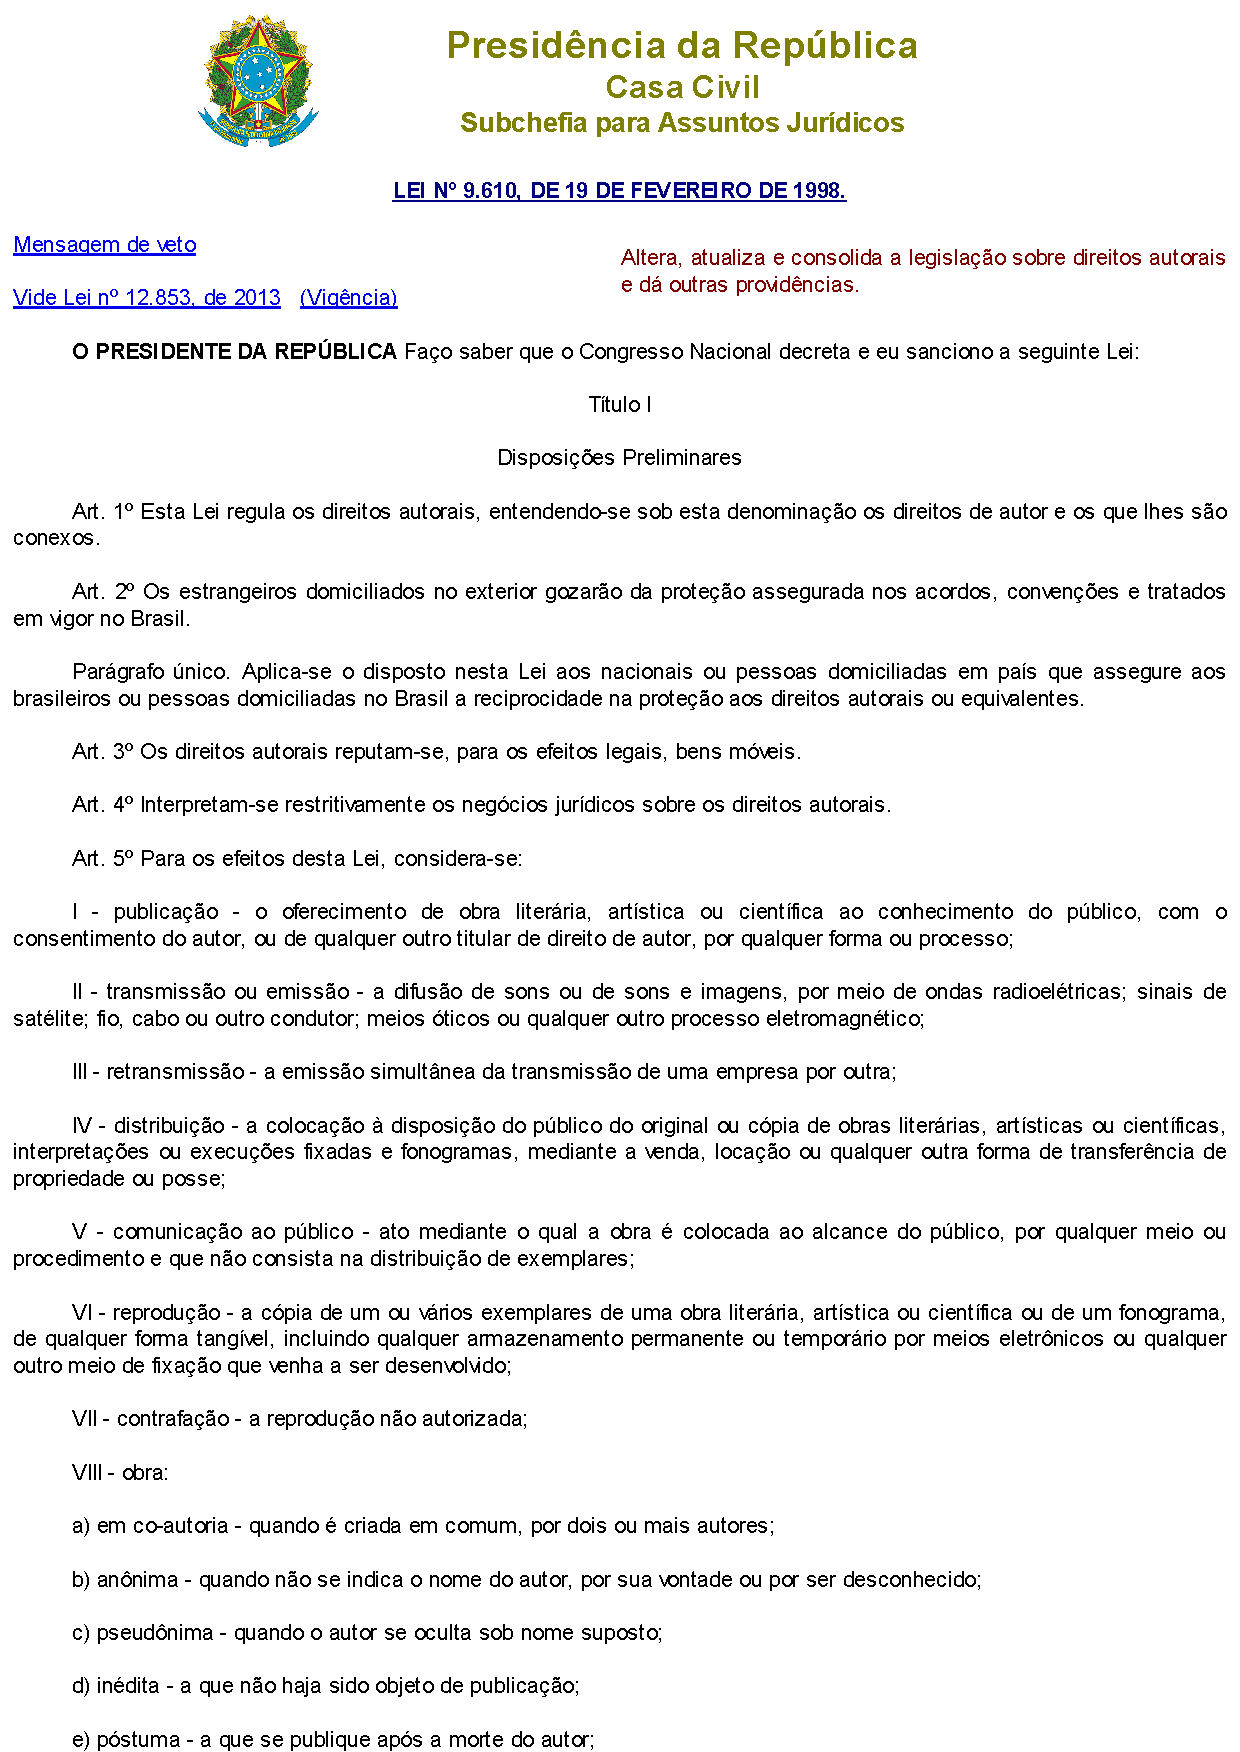
\includegraphics[width=\textwidth]{./PosTexto/Ilustracoes/lei-n9610-p1}}%% Imagem (Dimensões e localização)

\centerline{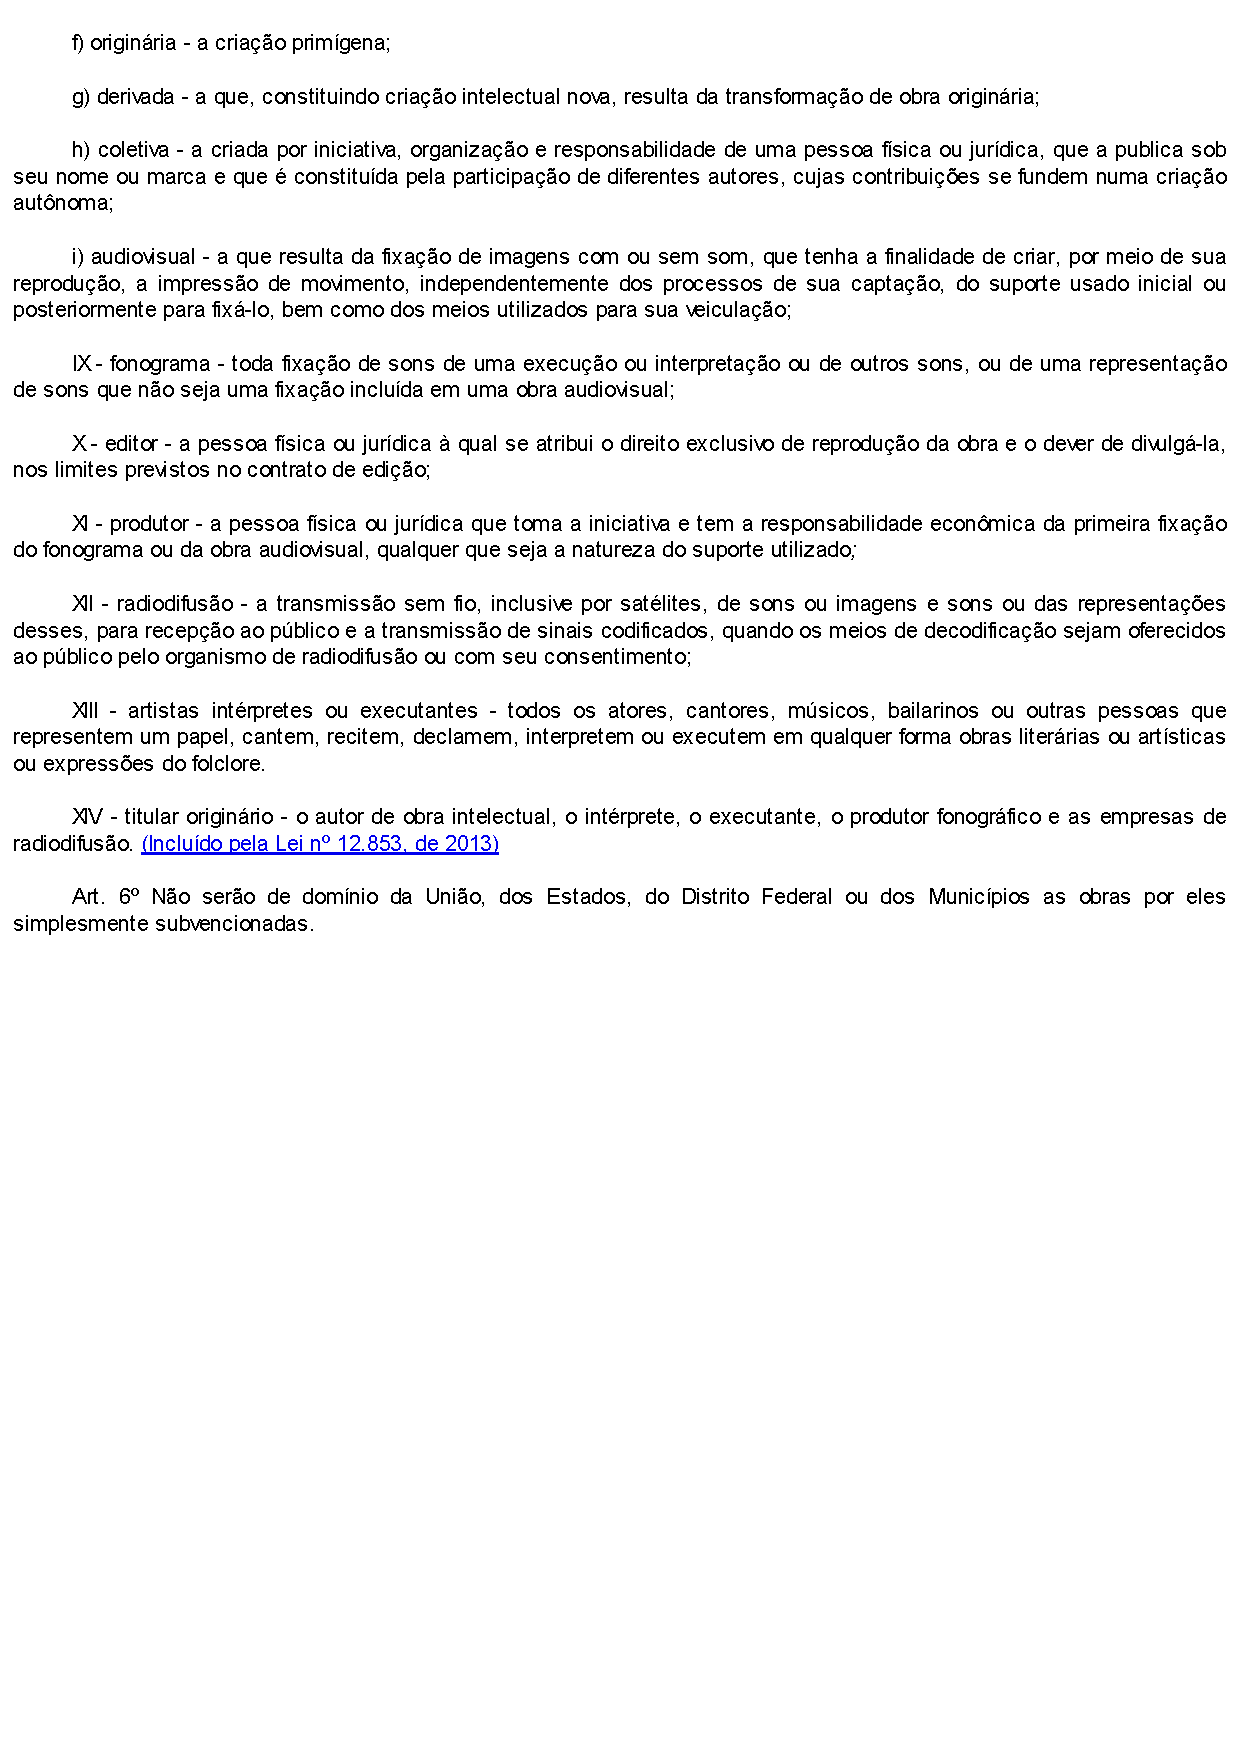
\includegraphics[width=\textwidth]{./PosTexto/Ilustracoes/lei-n9610-p2}}%% Imagem (Dimensões e localização)
%% Anexo - Comente para remover este item
  % %%%% ANEXO B
%%
%% Texto ou documento não elaborado pelo autor, que serve de fundamentação, comprovação e ilustração.

%% Título e rótulo de anexo (rótulos não devem conter caracteres especiais, acentuados ou cedilha)
\chapter{Normas para Elaboração de Trabalhos Acadêmicos}\label{cap:anexob}

As normas da \gls{utfpr} podem ser acessadas em: \url{http://portal.utfpr.edu.br/biblioteca/trabalhos-academicos/discentes/orientacao-para-trabalhos-academicos}. Ver Figura \ref{fig:capadolivro}.

\begin{figure}[htb]%% Ambiente figure
\captionsetup{width=0.9\textwidth}%% Largura da legenda
\caption{Sítio: Normas para Elaboração de Trabalhos Acadêmicos.}%% Legenda
\label{fig:capadolivro}%% Rótulo
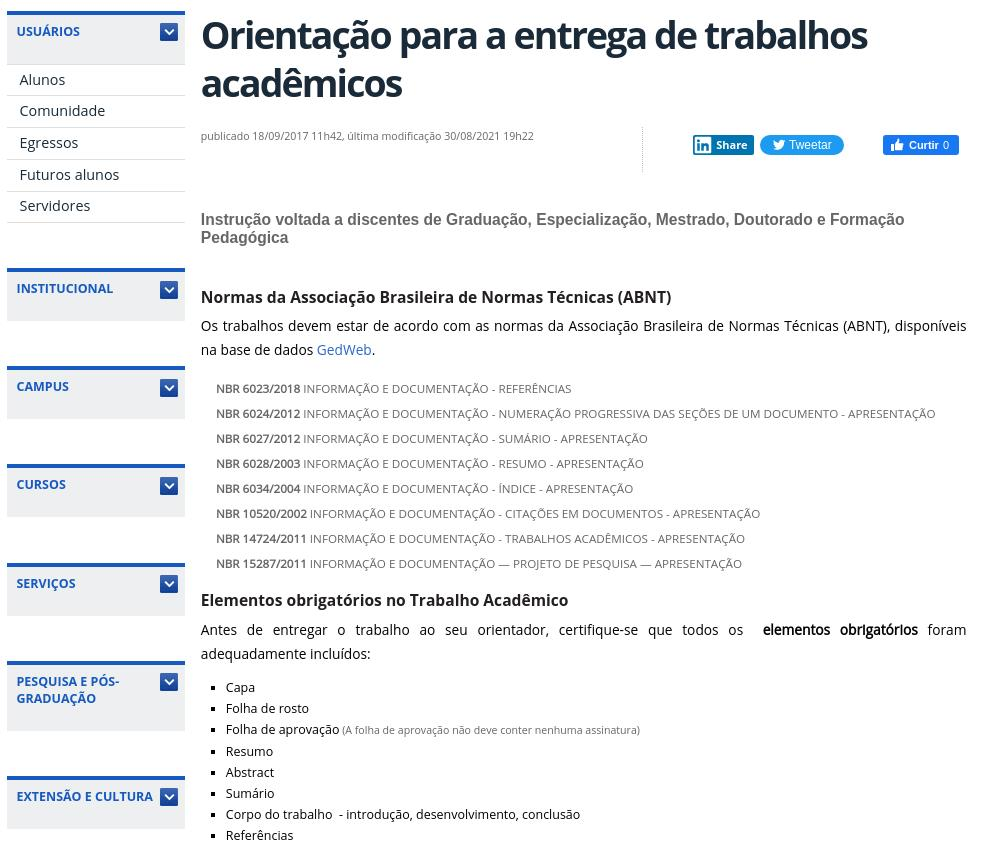
\includegraphics[width=0.9\textwidth]{normas}%% Dimensões e localização
\fonte{\cite{UTFPR2008}}%% Fonte
\end{figure}

%% Anexo - Comente para remover este item
\end{arquivosdeanexos}%% Não comente esta linha

%% Índice - Adiciona um índice remissivo.
%\incluirindice%% Comente para remover este item

%% Fim do documento
\end{document}%% Não comente esta linha
